%!TEX encoding = IsoLatin

%
% Exemple de rapport
% par Pierre Tremblay, Universite Laval
% modifié par Christian Gagne, Universite Laval
% 14/01/2011 - version 1.3
% modifié par Robert Bergevin, Université Laval
% 24/11/2011
% modifié par Jean-Yves Chouinard, Université Laval
% 11/01/2016
% modifié par Jean-Yves Chouinard, Université Laval
% 04/01/2017
%

%
% Modele d'organisation d'un projet LaTeX 
% rapport/      dossier racine et fichier principal
% rapport/fig   fichiers des figures
% rapport/tex   autres fichiers .tex
%

% ** Preambule **
%
% Ajouter les options au besoin :
%    - "ULlof" pour inclure la liste des figures, requis si "\begin{figure}" utilise
%    - "ULlot" pour inclure la liste des tableaux, requis si "\begin{table}" utilise
%
\documentclass[12pt,ULlof,ULlot]{ULrapport}

% Chargement des packages supplementaires (si absent de la classe)
\usepackage[utf8x]{inputenc}
\usepackage[autolanguage]{numprint}
\usepackage{icomma}
\usepackage{rotating}
\usepackage{wrapfig}
\usepackage{enumitem}
\usepackage{amsmath}
\usepackage{gensymb}
\usepackage{multirow}
\usepackage{multicol}
\usepackage{longtable}


%\usepackage[options]{nom_du_package}

% Definition d'une commande pour presenter des cellules multilignes dans un tableau
\newcommand{\cellulemultiligne}[1]{\begin{tabular}{@{}c@{}}#1\end{tabular}}

% Definition de colonnes en mode paragraphe avec alignement ajustable
% Cette definition requiert le chargement du package "array"
%    - alignement horizontal, parametre #1 : - \raggedright (aligne a gauche)
%                                            - \centering (centre)
%                                            - \raggedleft (aligne a droite)
%    - alignement vertical, parametre #2 : - p (aligne en haut)
%                                          - m (centre)
%                                          - b (aligne en bas)
%    - largeur, parametre #3 : longueur
\newcolumntype{Z}[3]{>{#1\hspace{0pt}\arraybackslash}#2{#3}}

% Definitions des parametres de la page titre
\TitreProjet{Fish \& Chips \\ Système autonome fixe pour le comptage et
l’identification de la faune marine}                         % Titre du projet
\TitreRapport{Rapport de projet -- version finale}                       % Titre du rapport
\Destinataire{Robert Bergevin, Luc Lamontagne et Simon Thibault}         % Nom(s) du destinataire
\NumeroEquipe{7}                                     % Numero de l'equipe
\NomEquipe{Les Requins}                               % Nom de l'equipe
\TableauMembres{%                                     % Tableau des membres de l'equipe
   111\,239\,483  & Vincent Lambert    & \\\hline        % matricule & nom & \\\hline
   111\,238\,936  & Rémi Lévesque & \\\hline        % matricule & nom & \\\hline
   111\,171\,798  & Ibrahim Mahamadou & \\\hline        % matricule & nom & \\\hline
   111\,233\,742  & Honoré Marcotte & \\\hline        % matricule & nom & \\\hline
   111\,160\,242  & Jérémy Talbot-Pâquet& \\\hline        % matricule & nom & \\\hline
}
\DateRemise{21 février 2019}                           % Date de remis


% Contenu de l'historique des versions
\HistoriqueVersions{%                        % Version & Date & Description \\\hline
         & 30 janvier 2019 & Création du document \\\hline
   0   & 31 janvier 2019 & Mise en page, ajout de la table des matières, des chapitres d'introduction et de description du projet\\\hline
   1   & 21 févier 2019 & Ajout du chapitre «Objectifs» et rédaction du cahier des charges\\\hline
   2   & 21 mars 2019 & Ajout du chapitre «Conceptualisation et analyse de faisabilité»\\\hline
   Finale   & 18 avril 2019 & Ajout des chapitres «Étude préliminaire» et «Concept retenu»\\
   \hline
}


% Corps du document

\begin{document}

%   Chapitres
%!TEX encoding = IsoLatin

%
% Chapitre "Introduction"
%

\chapter{Introduction}
\label{s:intro}

Avec les avancements technologiques des dernières décennies, l'accès à la donnée devient un besoin de plus en plus grandissant. Avoir sous la main des statistiques précises dans un certain secteur d'activité rend la tâche grandement plus facile dans l'optimisation d'un produit ou d'un service pour les firmes d'ingénierie. Avec ce nouvel accès à l'information, il est maintenant possible de cibler avec exactitude les besoins d'un client, multiplier la vitesse de production d'un service et même rendre des procédés complètement automatisés.

Dans le projet Fish \& Chips, il sera justement question de développer un design conceptuel d'un capteur permettant la documentation de la faune aquatique dans un milieu donné.

Le mandat fourni par le ministère de la Faune Aquatique impose donc une identification précise des populations de poissons, une collecte fiable d'images à des fins statistiques ainsi que l'accès à une base de données. Bref, le développement de ce produit pourra se traduire en deux principaux aspects : l'implantation d'un logiciel capable de fournir des données avec une fiabilité et une sécurité accrues, et la création d'un concept de capteur multidisciplinaire qui répond aux standards de qualité du client. 

D'abord, ce rapport présente la description du projet ainsi que les besoins et objectifs recherchés. Puis, il aborde le cahier des charges, la conceptualisation et l’analyse de faisabilité, l’étude préliminaire et le concept retenu de la solution présenté au Ministère de la Faune Aquatique.






%!TEX encoding = IsoLatin

%
% Chapitre "Structure d'un rapport technique"
%

\chapter{Description}
\label{s:structure_rapport}

Dans l’optique d’améliorer la fiabilité des données de suivi des populations de poissons, le Ministère de la Faune Aquatique souhaite mesurer l’activité marine sur différents sites sauvages et commerciales. À l’aide du projet pilote Fish \& Chips, le Ministère souhaite trouver une solution qui comblerait l’ensemble de ses besoins. M. Bergevin a d’ailleurs été chargé par le Ministère pour trouver le design conceptuel le plus adapté et le plus efficace parmi les firmes d’ingénieurs. C’est pourquoi la firme d'ingénieur des Requins devra se pencher sur ce mandat et proposer une solution fiable qui respectera l'ensemble des besoins du client.

Afin de respecter les demandes du Ministère, il est nécessaire de concevoir un système autonome afin de dénombrer et de documenter la faune aquatique. Ce nouveau système se doit d’identifier et de comptabiliser différentes espèces de poissons à tout moment. L'ensemble des activités du système doivent également garantir une mesure passive, c'est-à-dire sans risque pour les poissons. Pour une durée de deux ans, le système se doit de compiler des données pour des raisons de validation et doit être facilement accessible par un opérateur. Les coûts et les délais nécessaires à la conception et la réalisation d'un tel système doivent être minimisés. Par ailleurs, l'importance de l'aspect esthétique du système est négligeable, dans la mesure où elle n'affecte pas la disponibilité du capteur.

%!TEX encoding = IsoLatin

%
% Chapitre "Objectifs"
%

\chapter{Besoins et objectifs}
\label{s:objectifs}

\section{Analyse des besoins}

Afin de bien saisir la demande du client et de lui fournir une solution appropriée, une analyse des besoins sera réalisée. 

\subsection{Capteur optique autonome}

Pour commencer, l'automatisation et l'autonomie seront au coeur de ce projet. Le design doit comprendre un capteur optique qui recueillera des images des poissons observés. Le capteur optique doit être en mesure de prendre des photos en couleur sans interventions humaines. Ainsi, le capteur doit être muni d'un dispositif de détection de mouvement. Les images prise suite à l'identification doivent également être envoyées avec certaines informations physiques, dont la date et l'heure, la température interne du système ainsi que la température de l'eau lors de la prise de la photo. Le capteur optique doit être fonctionnel pour une durée minimale de deux semaines avant d'avoir recours à une maintenance. De plus, le capteur se doit d'être opérationnel en tout temps. Or, la caméra utilisée devra être d'une qualité suffisante pour permettre la reconnaissance du poisson, et ce, même la nuit.

\subsection{Système d'identification des poissons}

Le système d'identification des poissons est l'un des principaux besoins du client. En effet, le client souhaite recueillir des statistiques et une certaine documentation sur la faune aquatique. Pour y arriver, le système doit être en mesure d'identifier et de comptabiliser un minimum de cinq espèces de poissons évoluant dans un milieu aquatique à partir d'une prise de mesure non invasive. Comme mentionné précédemment, il est nécessaire d'assurer l'automatisation de l'identification des poissons.

%Le système se devra donc d'avoir un dispositif lui permettant de savoir quand prendre des photos et savoir si la photo contient bel et bien un poisson. L'enregistrement des données doit aussi se faire automatiquement. Après la collecte de données, le système sera tenu de stocker les données par lui-même pour une durée minimale de deux ans. Ensuite, il faudra gérer l'identification des poissons. Pour que le système soit efficace, il devra être en mesure d'identifier jusqu'à cinq variétés de poissons différentes, et ce, sans intervention humaine. Dans la même lancée, le système devra être autonome pour effectuer ces fonctions. 

\subsection{Interaction et sécurité du système}

L'interaction avec le système est primordiale afin de gérer les données du système et de recueillir les statistiques désirées. Le système doit permettre à l'usager de configurer et d'assurer les opérations du capteur à distance. Plus concrètement, l'utilisateur devra être capable d'avoir accès aux données en tout temps, et ce, peu importe sa localisation. Un serveur doit donc être implémenté pour permettre à l'usager de communiquer au capteur et ses archives sous une connexion sécurisée. En effet, par souci de confidentialité des renseignements et des données, toutes les connexions devront être sécurisées. Seul un utilisateur ayant une autorisation pourra communiquer avec le système. L'opérateur du capteur doit également pouvoir interagir avec le capteur à l'aide d'une interface locale.

Afin d'assurer la sécurité, le système doit être capable de générer des alarmes. Celles-ci seront acheminées vers l'opérateur du système en cas de défaillance de certaines fonctionnalités. 

\subsection{Archives des données}

Afin de collecter les informations et les statistiques du site aquatique, le système doit être muni d'un dispositif d'entreposage des données. Les archives devront comprendre certains éléments. D'abord, suite à l'identification des poissons, les images originales doivent être stockées dans le système à des fins de traitements et de validation ultérieur. Elles devront également être stockée avec leur vignette, soit les conditions enregistrées lors de la prise de la photo. De plus, les alarmes, les paramètres de configuration et les commentaires relevés par le responsable du capteur devront être archivés. L'ensemble de ces informations doivent être entreposées et accessibles pour une durée de deux ans.

\newpage{}

\section{Objectifs}

\begin{enumerate}

    \item Assurer un produit de qualité
    \begin{itemize}
        \item Maximiser la durée de vie de l'appareil
        \item Maximiser la précision et l'exactitude du logiciel de reconnaissance 
        \item Optimiser l'utilisation de l'interface graphique
        \item Maximiser les variétés de poissons identifiables
        \item Maximiser la capacité de stockage des données
        \item Maximiser la fiabilité du système de sécurité
    \end{itemize}
    
    \item Assurer le respect des contraintes
    \begin{itemize}
        \item Assurer une mesure passive du système
        \item Assurer le respect des contraintes mécaniques en milieu marin
        \item Assurer le respect des contraintes reliées aux images
    \end{itemize}

    \item Minimiser l'intervention humaine
    \begin{itemize}
        \item Maximiser la durée de vie de la batterie
        \item Minimiser la complexité de la maintenance
        \item Maximiser l'automatisation du transfert des données
        \item Faciliter l'accès à distance
    \end{itemize}
    
    \item Maximiser la facilité de conception
    \begin{itemize}
        \item Minimiser le temps de conception du produit
        \item Minimiser la complexité de l'usinage des pièces
        \item Faciliter la rechange des pièces
        \item Faciliter l'implantation du capteur sur différents sites
    \end{itemize}
    
    \item Minimiser les coûts
    \begin{itemize}
        \item Minimiser les coûts de conception du produit
        \item Minimiser les frais d'installation
        \item Minimiser les frais de maintenance et d'opération
        \item Minimiser le coût de remplacement des pièces
        \item Respecter les contraintes lié coûts globaux
    \end{itemize}
    
    \newpage
    
    \begin{figure}
        \centering
        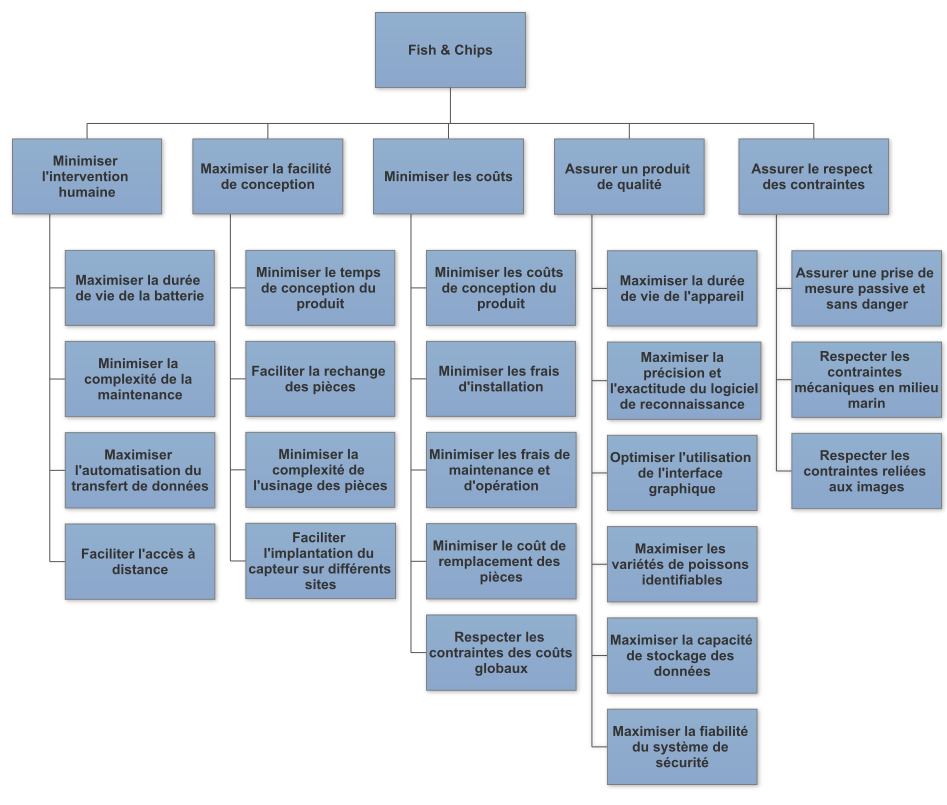
\includegraphics[width=1.0\linewidth]{fig/Organigramme.png}
        \caption{Organigramme des objectifs du projet Fish \& Chips}
        \label{fig:organigramme}
    \end{figure}
    
    %\item Autres (je sais pas dans quelle catégorie les mettre)
    %\begin{itemize}
    %    \item Maximiser la disponibilité du capteur
    %    \item Maximiser la sécurité
    %    \item Assurer une mesure passive
    %\end{itemize}
    
\end{enumerate}

%!TEX encoding = IsoLatin

%
% Chapitre "Cahier des charges"
%

\chapter{Cahier des charges}
\label{s:cahier_des_charges}

\section{Tableau des critères}
Cette section est destinée à la présentation des critères par rapport aux objectifs énoncés. La relation entre les critères et les objectifs sont présentés à la figure \ref{fig:maison_qualite}. Tel qu'affiché dans le tableau \ref{t:criteres}, une pondération est attribuée à chaque critère afin comparer leur importance. Un barème est également offert pour chacun des critère afin d'évaluer les concepts de solution.  

\begin{table}[htp]
   \footnotesize
   \centering
   \scalebox{1.0}{
   \begin{tabular}{|c|c|c|c|c|}
        \hline
        Critères & Pondération & Barème & Min. & Max.\\
        \hline
        \hline
        Qualité du produit & 65\% & & &\\
        \hline
        Résolution du capteur [Mpx] & 10\% & Éq. \ref{eq:bareme_res} & 10000 & $\infty$ \\
        Identification des poissons [poissons] & 10\% & Éq.  \ref{eq:bareme_identification} & 5 & $\infty$ \\
        Volume d'analyse [m$^3$] & 5\% & Éq. \ref{eq:bareme_volume_analyse} & 1 & $\infty$\\
        Capacité de stockage des données [Go] & 5\% & Éq. \ref{eq:bareme_stockage} & 200 & $\infty$ \\
        Durée de vie de l'alimentation du système [jours] & 5\% & Éq. \ref{eq:bareme_duree_batterie}  & 14  & $\infty$\\
        Acheminement des informations [m] & 5\% & Éq. \ref{eq:bareme_acheminement_infos} & 53 & 284 \\
        Fiabilité du système de sécurité & 5\% & Éq. \ref{eq:bareme_sécurité} & & \\
        Résistance à la profondeur [m] & 4\% & Éq. \ref{eq:bareme_profondeur} & 15.25 & 280 \\
        Taille des spécimens observés [cm] & 4\% & Éq. \ref{eq:bareme_taille_poisson} & 0 & $\infty$ \\
        Nombre de fonctionnalités de l'alarme & 4\% & Éq. \ref{eq:bareme_etat_systeme} & 0 & $\infty$\\
        Puissance de calcul & 4\% & Éq. \ref{eq:bareme_gpu} & 0 & 198 \\
        Utilisation de l'interface graphique & 4\% & Table \ref{t:bareme_interface} & & \\
        \hline\hline
        Performance & 20\% & & & \\
        \hline
        Précision du logiciel de reconnaissance [\%] & 15\% & Éq. \ref{eq:bareme_precision} & 0 & 100\\
        Précision de la régulation [$\%_\text{écart}$] & 2\% & Éq. \ref{eq:bareme_regul} & 0 & $\infty$\\
        Précision de la mesure de température [$\%_\text{écart}$] & 2\% & Éq. \ref{eq:bareme_precision_temperature} & 0 & $\infty$\\
        Précision de la mesure du temps [s] & 1\% & Éq. \ref{eq:bareme_precision_temps} & 0 & $\infty$\\
        \hline\hline
        Coûts & 15\% & & &\\
        \hline
        Coût de main d'oeuvre [\$] & 12\% & Éq. \ref{eq:bareme_cout_logiciel} & 0 & 40 000\\
        Coûts du matériel [\$] & 3\% & Éq. \ref{eq:bareme_cout_materiel} & 0 & 10 000 \\
%        \hline\hline
%        Respect des contraintes & 10\% & & & \\
%        \hline
%        Prise de mesure passive & 2\% & Table \ref{t:bareme_systeme_passif} & & \\
%        Masse du capteur [kg] & 2\% & Éq. \ref{eq:bareme_masse_capteur} & 0 & 5 \\
%        Volume du capteur [m$^3$] & 2\% & Éq. \ref{eq:bareme_volume_capteur} & 0 & 0.3\\
%        Résistance à la température [°C] & 2\% & Table \ref{t:bareme_resistance_temperature} & -6 & 30\\
%        Température mesurable [°C] & 2\% & Éq. \ref{eq:bareme_mesure_temperature} & -6 & 30\\
        \hline
   \end{tabular}}
    \caption{Table des critères du projet Fish \& Chips}
    \label{t:criteres}
\end{table}



\newpage{}

\section{Assurer la qualité de conception}
Les critères présents dans cette section représentent une pondération de 50\% du projet. Ces critères permettent de distinguer la qualité des concepts de solution.  

\subsection{Résolution du capteur}

%\begin{wrapfigure}{R}{6cm}
%    \centering
%    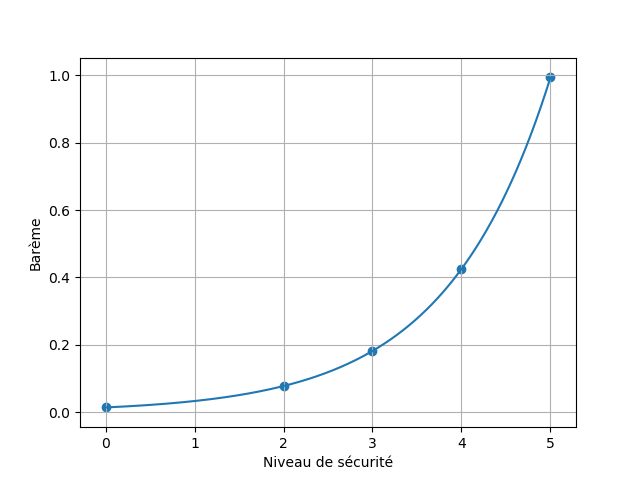
\includegraphics[width=\linewidth]{fig/Securite.png}
%    \caption{Illustration du barème du système de sécurité}
%    \label{fig:bareme_securite}
%\end{wrapfigure}

La résolution du capteur est un aspect important du projet. En effet, une pondération de 10$\%$ lui est attribuée puisque cette caractéristique aura un impact direct sur la capacité de reconnaissance ainsi que sur la qualité des vignettes dans la base de données. Le barème a été conçu à partir d'une fonction exponentielle puisque la différence entre 2 capteurs de résolution inférieure à 8 Mpx doit être significative selon le barème. À l'inverse, en comparant deux capteurs ayant des résolutions supérieures à environ 10 Mpx, la différence importe peu puisque la résolution est jugée suffisante pour les besoins du projet. Puisque les vignettes doivent avoir une taille de 100 par 100 pixels minimalement, la résolution minimale admissible est de 10000 px. Pour trouver la fonction du barème, il a été jugé qu'une résolution de 12 Mpx donnait une note de 0.8 au barème, puisqu'il s'agit d'une résolution suffisante pour le projet.

\begin{equation}
    y = \begin{cases}
        - e^{-0.134(x-0.01)}+1 &  \text{ si } x \geq 0.01 \\
        \text{Rejeté} & \text{ si } x < 0.01
        \end{cases}
    \label{eq:bareme_res}
\end{equation}
où $x$ est la résolution du capteur en Mpx.

\begin{figure}[!htb]
    \centering
    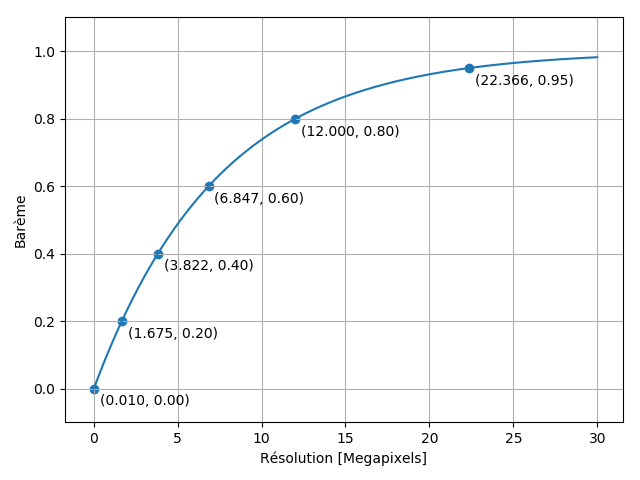
\includegraphics[width=0.45\linewidth]{fig/bareme_resolution.png}
    \caption{Barème pour la résolution du capteur}
    \label{fig:bareme_resolution}
\end{figure}



\subsection{Identification des poissons}

\begin{figure}[!htb]
    \centering
    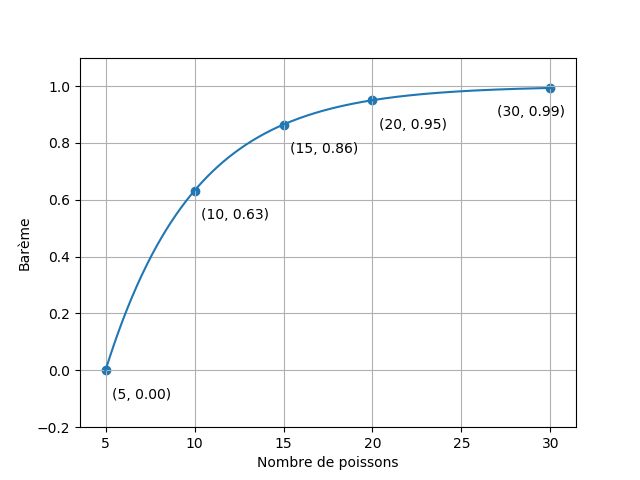
\includegraphics[width=0.45\linewidth]{fig/bareme_identification.png}
    \caption{Barème pour le nombre de poissons à identifier}
    \label{fig:bareme_identification}
\end{figure}

La quantité de poissons reste également à considérer dans l'implantation du système dans la mesure où deux sites différents peuvent chacun comporter une faune aquatique distinctive. Une optimisation de la taille de la librairie des poissons est d'une grande importance lors de la collecte des données par l'appareil: ce dernier doit évidemment être en mesure d'effectuer une bonne reconnaissance du type de poisson. On donnera donc à cette session une pondération de 10\%. Une variété de poisson trop stricte de la librairie causerait une collecte de données erronées dans certain milieux. Il est aussi à noter que le nombre de poissons à considérer est de cinq par site. On définira une équation exponentielle pour la gradation de ce barème: la clé du succès de ce critère repose dans la maximisation du nombre de poisson reconnaissables par la caméra. Par contre, on accordera graduellement moins d'importance à ce critère si le logiciel accepte déjà une grande quantité d'espèces marines. Avec un tel barème, on peut ainsi assurer la compatibilité du logiciel pour son implantation dans différents sites où la faune aquatique pourrait varier.

\begin{equation}
    y(x) = \begin{cases}
        -e^{-0.2(x-5)} + 1 & x \geq 5 \\
        \text{Rejeté} & \text{ si } x < 5 
    \end{cases}
    \label{eq:bareme_identification}
\end{equation}

\subsection{Volume d'imagerie}

Le volume d'imagerie est le volume dans lequel il est possible de prendre des mesures. Plus celui-ci est grand, plus il y de chance qu'il y aura un poisson et plus il sera facile de récolter les mesures. C'est pourquoi il est dans notre intérêt de le maximiser.

Selon les demandes du MFA, le volume minimal d'imagerie doit être de 1m$^3$. Le barème a la forme d'une fonction exponentielle puisqu'il permet d'inclure les systèmes  qui peuvent imager des objets très lointains, ce qui donnerait un volume d'imagerie infini. De plus, à partir de 5m$^3$, le volume d'imagerie est assez grand et avoir un volume d'analyse plus grand n'offre plus un avantage significatif. La fonction a été trouvée à partir des deux points $(1, 0)$ et $(5, 0.8)$.

\begin{equation}
y(x) = \begin{cases}
        -e^{-0.4024(x-1)}+1 & \text{ si } x \geq 1\\
        \text{Rejeté} & \text{ si } x < 1
    \end{cases}
    \label{eq:bareme_volume_analyse}
\end{equation}


\subsection{Capacité de stockage des données}
\label{subsection:capacite_stockage}

La collecte de données est un aspect primordial dans l'énonciation des critères imposés par le ministère: il est impératif que la taille de stockage puisse accepter des données allant jusqu'à une période de deux ans, et ce, à des fins de vérification. Le capteur peut avoir une résolution variant de 0 à 40 Mpx. Par contre, plus de pixels signifie moins de signal par pixel et il ne faut pas oublier que le capteur doit être capable d'opérer la nuit. Ainsi, on considère que la meilleure résolution soit de 12 Megapixels. En supposant que le système stockera en mémoire environ 20 photos par jour pendant 2 ans et que la taille d'un fichier serait de 12$\cdot 10^6$ octets, la capacité minimale de l'espace de stockage devra être de 175 Go. On arrondit ce chiffre à 200 Go pour être conservateur puisqu'il s'agit d'une estimation et que l'on stocke d'autres données supplémentaires comme la température et l'heure. On estime ensuite qu'un système pouvant enregistrer jusqu'à 1000 Go aura une note de 0.8. En utilisant un barème sous la forme exponentielle, on obtient l'équation \ref{eq:bareme_stockage}.

\begin{equation}
    y(x) = \begin{cases}
        -1.5e^{-0.002012x} + 1 & x \geq 200  \\      \text{Rejeté} & \text{ si } x < 200
    \end{cases}
    \label{eq:bareme_stockage}
\end{equation}


\subsection{Durée de vie de l'alimentation du système}

Dans l'objectif d'atteindre une autonomie minimale de deux semaines, il est nécessaire d'optimiser le système d'alimentation du capteur. % De plus, afin de ne pas limiter la disponibilité du capteur, il est idéal d'utiliser une batterie à cet effet. Une batterie rechargeable permettrait également d'augmenter significativement la durée de vie du capteur optique.
La durée de vie minimale demandée est de deux semaines. On considère que la composante chargée d'alimenter le système a une note de 0.8 si celui-ci est en mesure d'accomplir deux cycles de 14 jours. De cette manière, l'opérateur possède un cycle additionnel en cas d'oubli de rechargement. L'autonomie de la durée de vie de l'alimentation est évaluée selon l'équation \ref{eq:bareme_duree_batterie}. Si le système ne peut fournir de l'alimentation au capteur pour une durée de 14 jours, celui-ci sera rejeté.

\begin{equation}
    y(x) = \begin{cases}
        -6.25 e^{-0.13089x}+1 & \text{ si } x \geq 14\\
        \text{Rejeté} & \text{ si } x < 14
    \end{cases}
    \label{eq:bareme_duree_batterie}
\end{equation}


\subsection{Acheminement des informations}

Le système doit être capable de fonctionner à des profondeurs pouvant atteindre les 15.25m sous l’eau. En estimant qu'un poste de contrôle se situe au maximum à 50m de la position du capteur au niveau de l'eau, la distance minimale pour acheminer les données serait d'environ 53m. Puisque le lac le plus profond a une profondeur d'environ 280m~\cite{Lac_walker}, On estime que le critère sera pleinement rempli si le système peut acheminer les données jusqu'à 284m. Ainsi, nous évaluerons ce critère selon l'équation \ref{eq:bareme_acheminement_infos} en utilisant le barème suivant avec $x$ comme étant la distance qui sépare le poste de contrôle local et le système en mètres (m). Si le système ne peut acheminer les informations au-delà de 53m, il sera rejeté automatiquement.

\begin{equation}
    y(x) = \begin{cases}
        \frac{x}{231} - \frac{53}{231} & \text{ si } 53 \leq x \leq 284\\
        \text{Rejeté} & \text{ si } x < 53
    \end{cases}
    \label{eq:bareme_acheminement_infos}
\end{equation}


\subsection{Fiabilité du système de sécurité}

%\begin{wrapfigure}{R}{6cm}
%    \centering
%    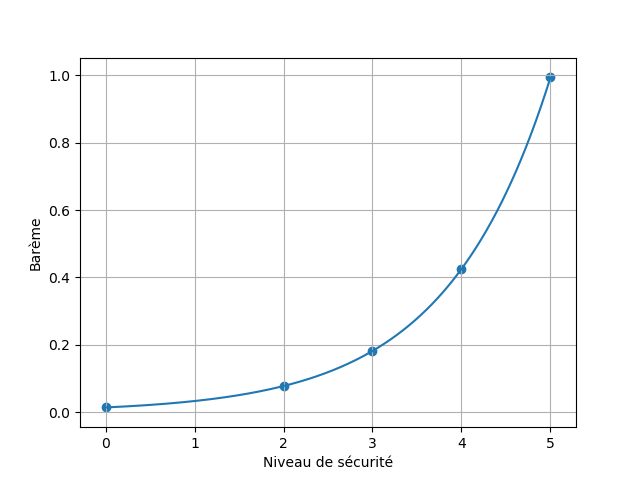
\includegraphics[width=\linewidth]{fig/Securite.png}
%    \caption{Illustration du barème du système de sécurité}
%    \label{fig:bareme_securite}
%\end{wrapfigure}

La confidentialité et l'authenticité des données est primordiale dans un tel projet: c'est pourquoi une grande partie de la cote associée à la qualité du design dépendra de la sécurité du produit. C'est pourquoi un 5\% de la note sera accordée à la sécurité. Plusieurs protocoles de conservation et de transfert des données devront être mis en place, et ce seront justement ici le nombre et la qualité des couches de sécurité offertes par le produit qui permettront une véritable quantification de ce critère. Puisque le système à livrer est fortement axé sur l'autonomie et l'accès à distance, un système qui est facilement compromis est à proscrire à tout prix. Une fonction exponentielle représente parfaitement l'enjeu ici: la moindre faiblesse du système de sécurité peut rendre le produit complètement inutilisable. Le niveau de sécurité $x$ est une combinaison du nombre de couches de sécurité pondéré par leurs qualités respectives.

\begin{equation}
    y = 0.849 e^{0.014x}
    \label{eq:bareme_sécurité}
\end{equation}

\subsection{Résistance à la profondeur du capteur}

La pondération attribuée à ce critère est de 2\%. Le MFA demande un capteur submersible jusqu'à 15.25m de profondeur au minimum. Sachant que le lac le plus profond au Québec est le Lac Walker avec une profondeur de 280m \cite{Lac_walker}, il est possible de déterminer un barème linéaire entre 15.25 et 280m tel que présenté à l'équation \ref{eq:bareme_profondeur}.

\begin{equation}
y(x) = \begin{cases}
        0.003777x-0.0557 & \text{ si } x \geq 15.25\\
        \text{Rejeté} & \text{ si } x < 15.25
    \end{cases}
    \label{eq:bareme_profondeur}
\end{equation}
où $x$ est la profondeur maximale à laquelle le capteur peut être submergé en mètres.

\subsection{Plage de température opérationnelle du capteur}

Une pondération de 2\% est attribuée à ce critère. Le MFA demande que le capteur opère dans une plage de +5°C et -10°C par rapport à l'eau. La température de l'eau peut varier de 4 à 25°C. Le capteur doit donc être opérationnel entre -6 et 30°C. Le barème pour ce critère est montré à la table \ref{t:bareme_resistance_temperature}.

\begin{table}[htp]
   \footnotesize
   \centering
   \begin{tabular}{|c|c|}
        \hline
        Résistance à la température & Barème\\
        \hline
        \hline
        Le capteur est opérationnel sur la plage de -6° à 30°C & 1.0 \\
        \hline
        Le capteur n'est pas opérationnel sur la plage de -6° à 30°C & Rejeté \\
        \hline
   \end{tabular}
   \caption{Barème de la plage de température opérationnelle du capteur}
   \label{t:bareme_resistance_temperature}
\end{table}


\subsection{Taille maximale des spécimens observables}

La pondération attribuée à ce critère est de 4\%. Le MFA demande de pouvoir imager des espèces qui ont une taille minimum de 6 cm. Ça veut dire qu'il faut être capable d'imager des poissons d'au minimum 6cm, mais c'est mieux si il est possible d'imager encore plus petit. Le barème à l'équation \ref{eq:bareme_taille_poisson} est établie selon une fonction exponentielle entre 0 et 6 cm puisqu'une différence entre 0.1 cm et 0.6 cm vaut moins qu'une différence entre 5 et 5.5 cm. Le barème est présenté à l'équation \ref{annexe:bareme_exp_poisson} où les paramètres $a$ et $b$ sont ajustés pour avoir la forme de courbe voulue.

\begin{equation}
y(x) = \begin{cases}
        \frac{1-10^{\frac{x-6}{6}}}{1-10^{-1}} & \text{si } x \leq 6\\
        \text{Rejeté} & \text{ si } x < 6
    \end{cases}
    \label{eq:bareme_taille_poisson}
\end{equation}
où $x$ est la taille minimale des spécimens observables en cm.

% Le capteur optique doit posséder une masse inférieure à 5kg sous l'eau. Le volume du capteur sous l'eau se doit de ne pas dépasser 0.3m$^{3}$. Le capteur doit être fonctionnel jusqu'à une profondeur de 50 pieds. Le système doit supporter une température entre +5°C et -10°C par rapport à la température de l'eau où le capteur sera situé.


\subsection{Nombre de fonctionnalités reliées à l'alarme}

La pondération associée à ce critère est de 2\%. En cas de problème au niveau du transfert de donnée ou de l'opération du capteur, le système doit envoyer une alarme à un responsable. Le nombre de fonctionnalités reliées à l'envoie de l'alarme différencie la qualité entre chaque concept d'alarme. Le dispositif de génération d'alarme doit avoir au minimum 1 fonctionnalité d'alarme. Il est convenu qu'au delà de 10 fonctionnalités, les concepts deviennent équivalents et qu'ils ont une note de 1. Le barème est présenté à l'équation \ref{eq:bareme_etat_systeme}.

\begin{equation}
    y(x) = \begin{cases}
    \frac{x-1}{9} & \text{ si } x \leq 10\\
    1 & \text{ si } x \geq 10\\
    0 & \text{ si } x < 1
    \end{cases}
    \label{eq:bareme_etat_systeme}
\end{equation}
où $x$ est le nombre de fonctionnalités reliées à l'alarme.

\subsection{Puissance de calcul}

La pondération de ce critère est de 2\%. La puissance de calcul sera déterminée par la performance de la carte graphique (source). Le barème est construit à partir d'un score qui reflète la vitesse moyenne effective de la carte graphique \cite{User_Benchmark_score}. La meilleure carte graphique a un score de 219 alors une note de 1 lui sera attribuée. Le barème sera établi de manière linéaire tel que montré à l'équation \ref{eq:bareme_gpu}.

\begin{equation}
    y = \frac{x}{219}
    \label{eq:bareme_gpu}
\end{equation}

\subsection{Utilisation de l'interface graphique}

\begin{table}[htb!]
   \footnotesize
   \centering
   \scalebox{0.8}{
   \begin{tabular}{|c|c|}
        \hline
        Difficulté de l'utilisation de l'interface & Barème \\
        \hline
        \hline
        Très facile & 1.0 \\
        \hline
        Facile & 0.8 \\
        \hline
        Intermédiaire & 0.6 \\
        \hline
        Difficile & 0.4 \\
        \hline
        Très difficile & 0.0 \\
        \hline
   \end{tabular}}
   \caption{Évaluation du barème de l'interface graphique}
   \label{t:bareme_interface}
\end{table}

Puisque l'optique principale de ce projet tourne autour une automatisation des tâches, l'aisance d'utilisation de l'interface lors de l'accès aux données et des opérations de maintenance bimensuelles rejoint tout autant la ligne directrice du design d'appareil (pondération de 5\%). La différenciation entre un interface graphique excellent et médiocre étant difficile à quantifier par calcul, on donnera un barème sous forme de charte, où la valeur la plus grande sera accordée à une qualification de "très intuitive" et la plus faible à "très difficile d'utilisation". La charte des barèmes est présentée à la table \ref{t:bareme_interface}. 


\section{Offrir un système performant}
La performance est un aspect important du projet. Cette section comprend des critères de précision afin d'assurer la performance du système. Une pondération de 20\% est attribué à l'ensemble des critères.

\subsection{Précision du logiciel de reconnaissance}

% \begin{wrapfigure}{R}{7cm}
\begin{figure}[htb!]
    \centering
    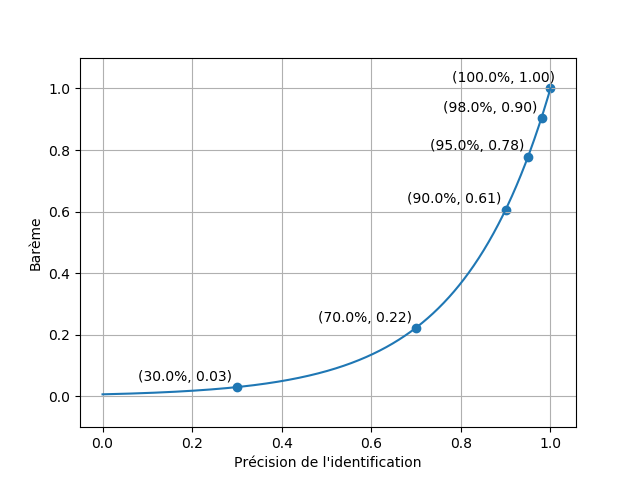
\includegraphics[width=0.45\linewidth]{fig/bareme_ident.png}
    \caption{Illustration du barème pour la précision de l'identification des poissons}
    \label{fig:bareme_precision}
\end{figure}
% \end{wrapfigure}

Le logiciel de reconnaissance du poisson étant au coeur du projet de conception, on donnera une certaine importance à la précision et l'exactitude du programme pour assurer une collecte de données efficace (pondération de 15\%). De plus, un logiciel incapable de faire une bonne différenciation des espèces de poissons ruine l'ensemble des investissements ultérieurs: une excellente caméra ne vaut rien sans un logiciel de qualité. Par contre, à une différenciation d'exactitude dans les très hauts pourcentages (85 à 100), on donnera graduellement moins d'importance aux variations d'efficacité. À un tel niveau d'exactitude, on laissera plus d'importance aux autres caractéristiques en considérant la précision de l'appareil déjà pratiquement maximisée. La fonction quantifiant la qualité de la reconnaissance du poisson s'apparente à une fonction de type exponentielle tel que présenté ci-contre:

\begin{equation}
    y = e^{5(x-1)}
    \label{eq:bareme_precision}
\end{equation}

\subsection{Précision de la température régulée}

La pondération attribuée à la précision de la régulation de la température est de 2$\%$. Le barème prend une forme exponentielle puisqu'un changement de précision près de 1$\%$ d'écart entraîne une plus grosse variation du barème qu'un écart autour de 50$\%$ d'écart. Les paramètres de la fonction exponentielle sont ajustés de manière à ce qu'un pourcentage d'écart de 0$\%$ donne 1 et un pourcentage d'écart de 50$\%$ donne 0.2.

\begin{equation}
    y(x) = e^{-0.03219x}
    \label{eq:bareme_regul}
\end{equation}
où $x$ est la pourcentage d'écart entre la température du système en régime permanent et la température désirée. Il s'agit donc d'un pourcentage d'erreur statique.

\subsection{Précision de la mesure de température}

La pondération attribuée à la précision de la régulation de la température est de 2$\%$. Le barème est basé sur une fonction exponentielle puisqu'il est généralement facile d'avoir une bonne précision pour mesurer la température. L'ajustement des paramètres est le même qu'à l'équation \ref{eq:bareme_regul} pour la régulation de la température.

\begin{equation}
    y(x) = e^{-0.03219x}
    \label{eq:bareme_precision_temperature}
\end{equation}
où $x$ est le pourcentage d'écart entre la température mesurée et la température réelle.

\subsection{Précision de la mesure du temps}

La pondération attribuée à la précision de la mesure du temps est de 1$\%$. Le barème est basé sur une fonction exponentielle puisqu'il prend en compte les très grandes erreurs sur la date et l'heure. L'ajustement des paramètres est fait de manière à ce qu'un écart nul donne une note de 1 et qu'un écart de 2 semaines ($1.2\cdot 10^6$s) donne une note de 0.2.

\begin{equation}
    y(x) = e^{-1.341\cdot10^{-6}x}
    \label{eq:bareme_precision_temps}
\end{equation}
où $x$ est l'écart absolue entre l'heure mesurée et l'heure réelle en secondes.

\section{Coûts}

Une limite des coûts a été établie : on ne peut dépasser 10 000 dollars de frais matériel et 40 000 dollars de coûts de main d'oeuvre. 

Le barème est fait de telle sorte qu'un budget alloué utilisé dans son entièreté donne une note de 0 dans le but de minimiser les coûts. À l'opposé, un coût nul offrirait une note de 1.

Ainsi, de manière générale, le barème pour un tel critère serait:

\begin{equation}
    y(x)=\frac{-x}{\text{Budget}} + 1
\end{equation}

\subsection{Coûts en main d'oeuvre}

\begin{equation}
y(x) = \begin{cases}
        \frac{-x}{40000} + 1 & \text{ si } x \leq 40000\\
        \text{Rejeté} & \text{ si } x > 40000
    \end{cases}
    \label{eq:bareme_cout_logiciel}
\end{equation}

\subsection{Coûts de conception du produit}

La première étape précédant l’utilisation de la machine, est sa conception. Cette partie est non négligeable dans le processus d’analyse des coûts de la machine car elle représente la plus grande source de dépense en matériaux. Afin de combler les besoins du Ministère, on cherche à minimiser les coûts totaux liés à la fabrication de la machine. %En parallèle, il faut limiter les coûts pour que le Ministère puisse économiser et favorisera ainsi le projet.
Ainsi, la fonction décrivant l’efficacité par rapport au coût de production suit une forme suivante :

\begin{equation}
y(x) = \begin{cases}
        \frac{-x}{10000} + 1 & \text{ si } x \leq 10000\\
        \text{Rejeté} & \text{ si } x > 10000
    \end{cases}
    \label{eq:bareme_cout_materiel}
\end{equation}

Un système ne respectant pas la limite de 10000\$ en coûts de matériel sera rejeté. Considérant l'importance du respect des coûts de conception, une pondération de 4\% a donc été attribué à ce critère.


%\section{Respect des contraintes}

%Afin que le concept de solution soit intéressant pour le client, il est nécessaire que chacun des critères concernant les mesures physiques soient respectés. Les critères présent dans cette section représente de nombreux besoins du client. Ainsi, une pondération de 15\% y est attribué. 

%\subsection{Prise de mesure passive}

%Bien que l'objectif principal du capteur est d'identifier une variété de poissons dans un milieu aquatique, il est nécessaire que cette identification n'affecte pas le mode de vie des poissons. En effet, l'une des principales motivations du client à l'égard du projet Fish \& Chips est d'assurer une mesure passive. Le capteur optique ne doit en aucun cas perturber l'environnement des poissons évoluant sur le site. Une importance relative de 2\% est donc accordée à ce critère. En cas de perturbation de l'environnement, le design est automatiquement rejeté, comme le précise la table \ref{t:bareme_systeme_passif}.

%\begin{table}[htp]
%   \footnotesize
%   \centering
%   \begin{tabular}{|c|c|}
%        \hline
%        Degré de passivité du système & Barème\\
%        \hline
%        \hline
%        Le système assure une mesure passive & 1.0 \\
%        \hline
%        Le système n'assure pas une mesure passive & Rejeté \\
%        \hline
%   \end{tabular}
%   \caption{Évaluation du barème du degré de passivité du système}
%   \label{t:bareme_systeme_passif}
%\end{table}

% \subsection{Contraintes mécaniques}

% Le capteur optique doit respecter certaines contraintes physiques et mécaniques. Le non respect de ces contraintes ne doit en aucun cas affecter les fonctionnalités du système. De plus, l'aspect physique du capteur optique ne doit pas être un facteur pouvant perturber l'environnement des poissons. C'est dans cette optique qu'on attribue aux contraintes mécaniques une pondération de 5\% de l'ensemble du projet. Ce barème a été calculé considérant le tableau \ref{eq:bareme_volume_capteur} et les caractéristiques suivantes:

%\subsection{Masse du capteur}

%Le MFA spécifie que le capteur optique doit posséder une masse inférieure à 5kg sous l'eau. Pour cette raison, un capteur ayant une masse supérieure à 5 kg sera rejeté. Le barème présenté à l'équation \ref{eq:bareme_masse_capteur} prend la forme d'une fonction cosinus pour que le barème ne varie pas beaucoup près de 0 et 5 kg puisqu'un design de capteur ayant une masse de 0 à 1 kg serait très bon et que deux designs de capteur ayant une masse entre 4 et 5 kg seraient presque équivalents. Par contre, le barème varie à peu près linéairement entre 1 et 4 kg. La fréquence du cosinus est ajustée de manière à ce qu'il y ait une demie période entre 0 et 5kg. La pondération attribuée à ce critère est de 2$\%$ étant donné que le plus important est tout simplement d'avoir une masse respectant la demande du client.

%\begin{equation}
%y(x) = \begin{cases}
%        1 & \text{ si } 0 \le x \leq 5\\
%        \text{Rejeté} & \text{ si } x > 5
%    \end{cases}
%    \label{eq:bareme_masse_capteur}
%\end{equation}
%où $x$ est la masse du capteur submergé en kg.

%\subsection{Volume du capteur}


%Selon la demande du client, le volume du capteur doit être inférieur à 0.3 m$^3$. L'équation \ref{eq:bareme_volume_capteur} pour le barème du volume du capteur a la même forme que l'équation \ref{eq:bareme_masse_capteur} pour les mêmes raisons citées ci-dessus. La seule différence est que les paramètres sont ajustés de manière à ce qu'un volume de 0.3m$^3$ donne une note de 0. La pondération attribuée à ce critère est de 2$\%$ puisqu'il est surtout important d'avoir un volume inférieur à 0.3m$^3$.

%\begin{equation}
%y(x) = \begin{cases}
%        1 & \text{ si }0 \le x \leq 0.3\\
%        \text{Rejeté} & \text{ si } x > 0.3
%    \end{cases}
%    \label{eq:bareme_volume_capteur}
%\end{equation}
%où $x$ est le volume du capteur submergé en m$^3$.


%\subsection{Intervalle de température mesurable}


%\begin{equation}
%y(x) = \begin{cases}
%    1 & \text{ si } -6 \leq x \leq 30\\
%    \text{Rejeté} & \text{Autrement}
%    \end{cases}
%    \label{eq:bareme_mesure_temperature}
%\end{equation}


%\begin{enumerate}
%    \item Le capteur optique doit posséder une masse inférieure à 5kg sous l'eau.
%    \item Le volume du capteur sous l'eau se doit de ne pas dépasser 0.3$m^{3}$. 
%    \item Le capteur doit être fonctionnel jusqu'à une profondeur de 50 pieds.
%    \item Le système doit supporter une température entre +5°C et -10°C par rapport à la température de l'eau où le capteur sera situé.
%\end{enumerate}


%   \begin{enumerate}
%       \item Les images capturées doivent être en couleur.
%       \item La taille des images ne doit pas excéder 8 bits.
%       \item Les dimensions des photos doivent être de 100 X 100 pixels.
%       \item Chacune des images recueillies doivent également fournir la date et l'heure, la           température interne du système, la température de l'eau et l'identification du poisson.
%       \item Le capteur optique doit être en mesure d'observer des spécimens de plus de 6cm.
%       \item Le système doit être en mesure de capter des poissons dans un volume minimal de           1$m^{3}$.
%    \end{enumerate}



%\section{Intervention humaine}

%En analysant les demandes du client, on se rend vite compte que l’automatisation du système sera un élément prépondérant dans notre système. Pour parvenir à un système autonome, il faudra impérativement tenir compte de certains aspects comme la  durée de vie de la batterie, l’automatisation des transferts de données, l’accès à distance ainsi que la complexité de la maintenance qu’il faudra minimiser afin de réduire au maximum l’intervention humaine. Compte tenu de l’importance de cet aspect dans le projet, l’équipe de conception attribue une pondération de 20\%.


\newpage


\section{Maison de qualité}

\begin{figure}[htb!]
    \centering
    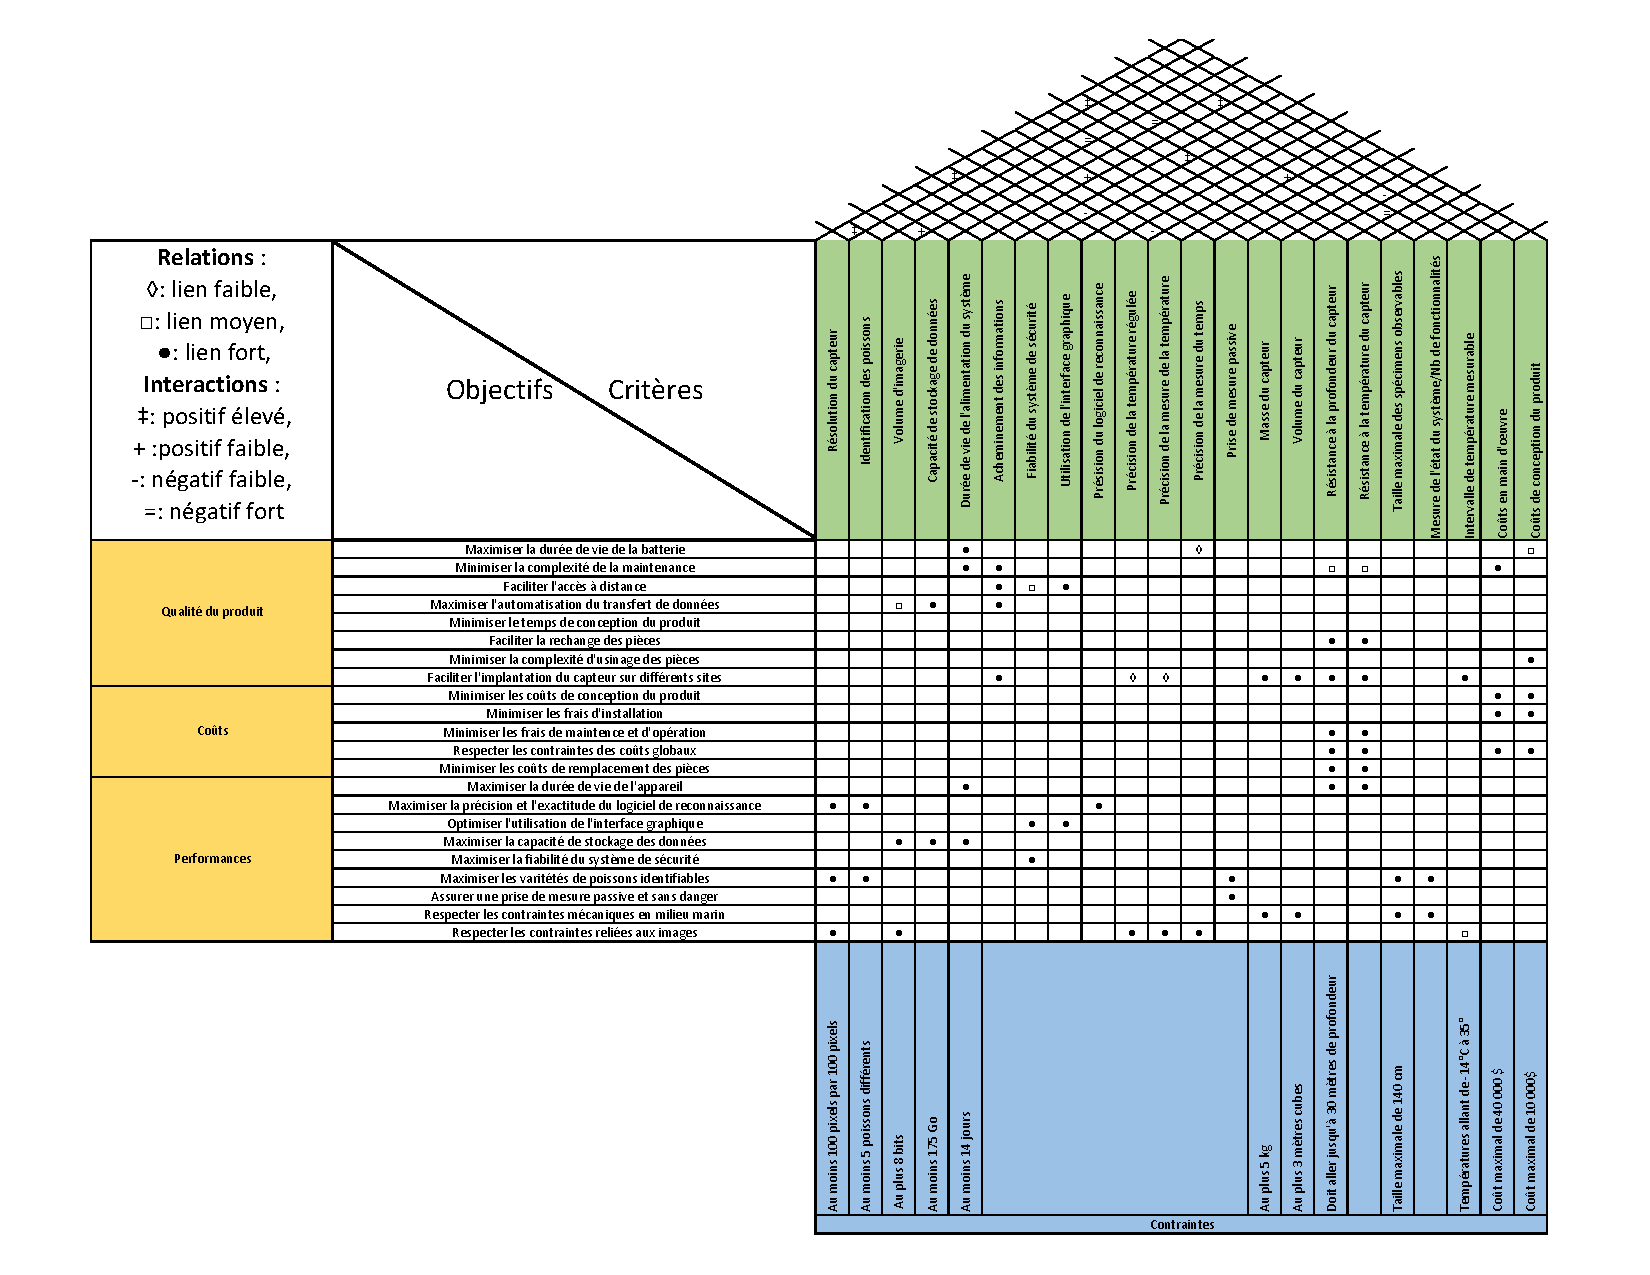
\includegraphics[width=\linewidth]{fig/MQ3.pdf}
    \caption{Maison de qualité du projet Fish \& Chips}
    \label{fig:maison_qualite}
\end{figure}

%!TEX encoding = IsoLatin

%
% Chapitre "Conceptualisation et analyse de faisabilité"
%

\chapter{Conceptualisation et analyse de faisabilité}
\label{s:conceptualisation_et_analyse}

\section{Diagramme fonctionnel}

\begin{figure}[!htb]
    \centering
    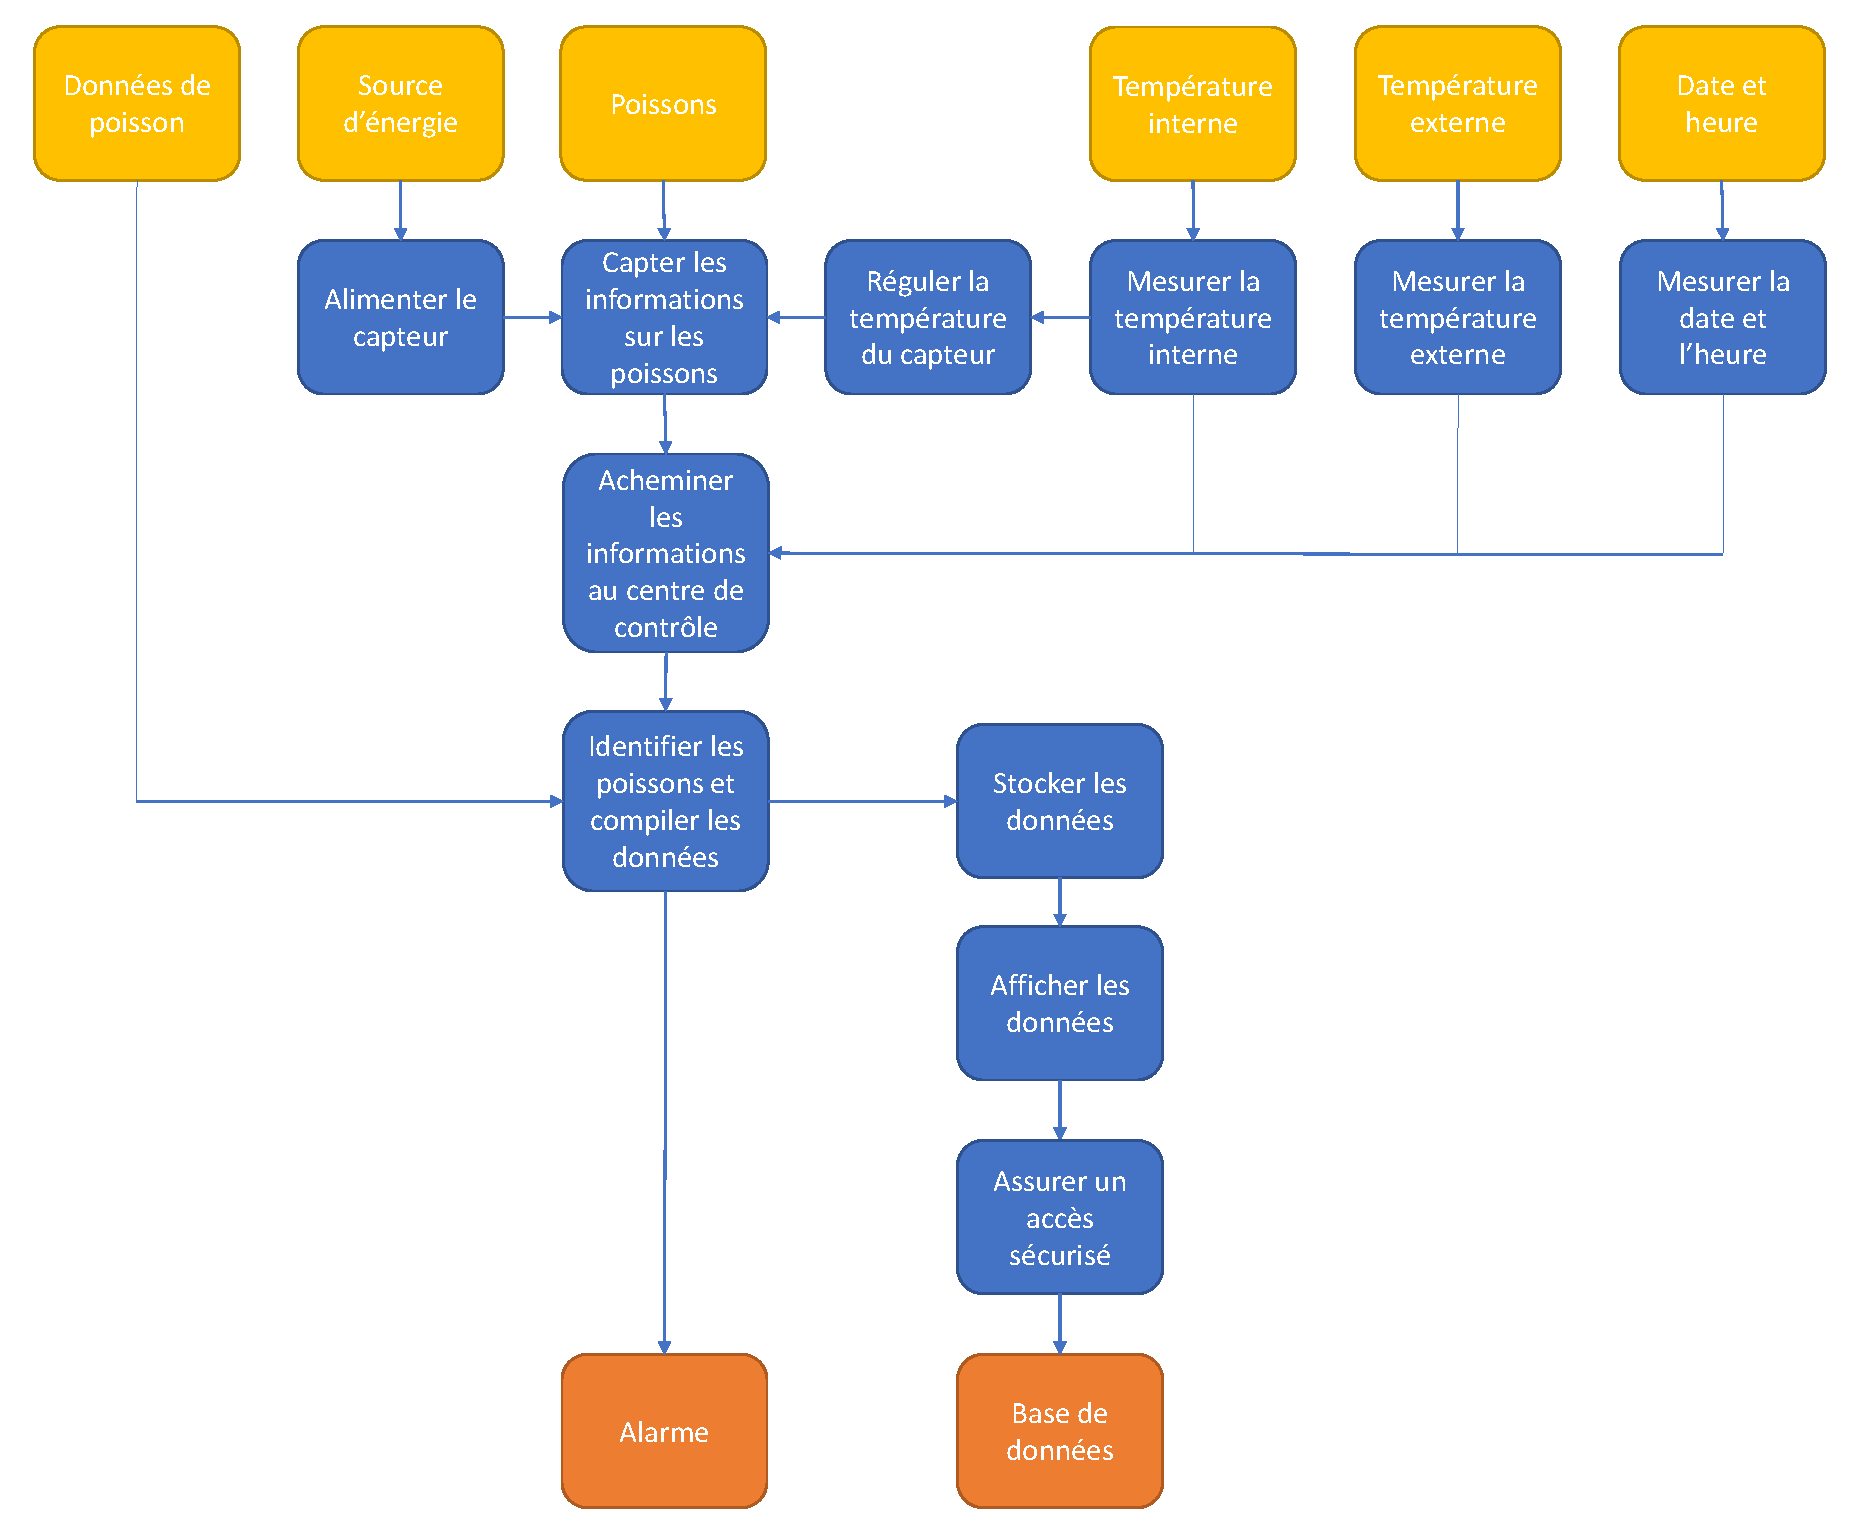
\includegraphics[width=0.80\linewidth]{fig/Diagramme_fonctionnel.pdf}
    \caption{Diagramme fonctionnel du projet Fish \& Chips}
    \label{fig:diagramme_fonctionnel}
\end{figure}

La figure \ref{fig:diagramme_fonctionnel} présente le diagramme fonctionnel du design pour le projet Fish \& Chips. Les intrants y sont présentés en jaune, les fonctions en bleu et les extrants en rouge.

Les intrants constituent toutes les données nécessaires au projet que l'on extrait de l'environnement. Les poissons sont au coeur du projet: à l'aide d'une mesure passive, ils devront être analysés et identifiés par un système de reconnaissance. Le MFA souhaite comptabiliser les espèces de poissons d'eau douce du Québec qui font plus de 6 cm de long. Pour ce faire, des données de poissons seront fournies au système de reconnaissance. Elles seront sous une forme de base de données qui comprendra plusieurs photos de poissons de chaque espèce sous différents angles de vue avec leur espèce correspondante. Cela servira à l'entraînement ou de référence au système d'identification. Ensuite, une source d'énergie sera tirée de l'environnement ou d'une composante pour alimenter le dispositif qui sera chargé de capter les données brutes sur les poissons. La température interne du dispositif de mesure des poissons, la température de l'eau ainsi que la date et l'heure sont nécessaires à la création de la vignette. De plus, certaines de ces données serviront à déterminer s'il y a une erreur dans le système pour avertir un utilisateur.

Les extrants du système sont les choses qui seront produites par le système. Le point central du design est de produire une base de données contenant toutes les vignettes de poissons identifiés, les statistiques sur les populations des différentes espèces, les images originales enregistrées pour une durée de 2 ans ainsi que d'autres informations connexes comme les commentaires, les paramètres de configuration et les alarmes. Les alarmes seront envoyées à un responsable sous la forme d'un message lui avertissant que le fonctionnement du système peut être compromis.

%\pagebreak

\section{Conceptualisation et analyse des solutions}

\subsection{Capter les informations sur les poissons}

Afin d'optimiser et de faciliter l'identification des poissons, il est nécessaire d'utiliser un système de détection de qualité. En ce sens, il est primordial que le capteur optique utilisé soit fiable et efficace. Le capteur optique a comme responsabilité de détecter les poissons de même que prendre une image de ceux-ci. Cependant, son utilisation ne doit en aucun cas perturber l'environnement de la faune aquatique.


\textbf{Aspects physiques:}
\begin{itemize}[label = {--}]
    \item Sous l'eau, la solution doit posséder une masse inférieure à 5kg.
    \item Sous l'eau, la solution doit posséder un volume de moins de 0.3m$^3$.
    \item La solution doit être utilisable jusqu'à une profondeur de 50 pieds.
    \item La température interne de la solution doit rester entre -6°C et 30°C.
\end{itemize}

\textbf{Aspects économiques:}
\begin{itemize}[label = {--}]
    \item La solution doit être la moins dispendieuse possible.
\end{itemize}

\textbf{Aspects temporels:}
\begin{itemize}[label = {--}]
    \item Le temps de développement de la solution doit être minimisé.
    \item Le temps de livraison de la solution doit être minimisé.
\end{itemize}

\textbf{Aspects socio-environnementaux:}
\begin{itemize}[label = {--}]
    \item La solution doit assurer une mesure passive.
\end{itemize}

\subsubsection{GoPro Hero7 Black Edition}

\textbf{Description:} La GoPro Hero7 Black comporte plusieurs fonctionnalités. Elle peut prendre des images de 12 méga-pixels à grande gamme dynamique (HDR) et des vidéos allant de 720p à 4K. La GoPro peut également prendre entre 24 et 240 images par secondes. Elle comprend un système de stabilisation d'images idéal pour la détection de poissons et un mode pour la vision nocturne. Sa fonctionnalité « Live Streaming » ainsi que son système de connexion Wi-Fi et Bluetooth intégré permettraient également de relever les données sur les poissons en temps réels. Un système intégré GPS permet de la localisé en tout temps. La GoPro est livrable entre 3 et 6 jours à des frais d'environ 560\$.

\textbf{Décision:} Retenu, mais.

\textbf{Justification:} La GoPro Hero7 Black Edition comporte de nombreux avantages et réponds aux exigences du client. En effet, la masse de la caméra est de 0,116kg et son volume est de 9,2309x10$^{-5}$m$^3$. Il s'agit d'une caméra très fiable et utilisée dans des conditions climatiques extrêmes. Cependant, la GoPro peut seulement atteindre une profondeur de 33 pieds. Des frais additionnels d'environ 67\$ sont donc nécessaire pour l'achat d'un boîtier de plongée permettant à la caméra d'atteindre une profondeur de 196 pieds. Malgré les coûts supplémentaires, la GoPro reste abordable comparé à ses concurrents sur le marché.

\textbf{Références:} \cite{GoPro_Specs} \cite{GoPro_Waterproof}


\subsubsection{HP2W Hyperfire 2 Professionnal White Flash Camera}
\label{subsubsectionHyperfire}

\textbf{Description:} Conçu pour la chasse, cette caméra offre beaucoup de fonctionnalités intéressantes dans le cadre du projet Fish \& Chips. La HP2W peut prendre des images de 3 méga-pixels et des vidéos de 720p à haute définition. La caméra peut ainsi prendre entre 5 et 450 images par secondes. Elle peut fonctionner à des températures allant de -40°F à +140°F et elle possède un détecteur de mouvements et un flash intégré pour la nuit. Son prix incluant les frais de livraison monte à environ 660\$.

\textbf{Décision:} Retenu, mais.

\textbf{Justification:} Cette caméra de chasse professionnelle répond à l'ensemble des exigences du projet. Elle possède une masse de 0,380kg et un volume de 1,0143x10$^{-3}$m$^3$. La HP2W respecte également les contraintes de températures. Aucune informations concernant l'étanchéité du produit est spécifié. Le boîtier est néanmoins capable de résister à des fortes tempêtes de pluie.

\textbf{Références:} \cite{HP2W}


\subsubsection{GoFishCam}

\textbf{Description:} La GoFishCam est une caméra utilisée pour la pêche. Elle peut enregistrer des vidéos de haute définition de 720p et de 1080p. Elle peut prendre entre 30 et 60 images par seconde. Cette caméra est conçue avec du matériel militaire et sa forme aérodynamique permet une stabilisation d'image lors de l'enregistrement. La GoFishCam comprend des diodes électroluminescentes (LEDs) efficace pour la vision de nuit. Son prix s'élève à environ 325\$ et est livrable entre 10 et 15 jours.

\textbf{Décision:} Retenu.

\textbf{Justification:} La GoFishCam comprend étonnamment des spécifications techniques adéquates pour le projet. En effet, la caméra peut atteindre une profondeur de près de 500 pieds et possède une masse de 0,094kg. La GoFishCam respecte également les contraintes reliées au volume. En effet, elle possède un volume d'environ 8,624x10$^{-5}$m$^3$. La caméra possède également un système de Wi-Fi intégré et une fonction « Live Stream » permettant la diffusion en directe sur une application.

\textbf{Références:} \cite{GoFishCam} 


\subsubsection{Capteur d'image OV5640}
\label{subsubsection:camera_custom}

\textbf{Description:} Cette solution permet de créer notre propre caméra à l'aide du capteur d'image CMOS OV5640 (modèle ELP-USB500W02M-AF60). Ce capteur permet d'enregistrer des images de 5 méga-pixel, dont la résolution maximale est de 2592x1944 pixels. Il peut prendre entre 15 et 30 images par seconde, et ce, en couleur et en haute définition. Le capteur peut prendre des images des objets situés entre 5cm et 100m de la lentille. Le «focus» de la lentille est d'ailleurs automatique. Ce capteur peut être opérationnel à des températures variant entre -20°C et 70°C. Un tel système est composé d'un senseur et d'une lentille pour imager sur le senseur. Ainsi, il s'agit d'un système simple, léger et complètement programmable par port USB. Par ailleurs, puisque le capteur ne peut être submergé, il aurait un boîtier fait en aluminium 2014-T6 et une fenêtre en PMMA\footnote{Communément appelé Plexiglas™} encastrée pour permettre de voir au travers comme montré à la figure \ref{fig:boitier_camera_custom}. Il serait contenu dans un volume de 0.04m$^3$ et il aurait une masse totale de 2.25kg avec les données de l'annexe \ref{annexe:equation_boitier}.

\textbf{Décision:} Retenu, mais.

\textbf{Justification:} Le principal avantage de la création d'un système de capture d'image est le coût. En effet, un tel système coûte seulement 60\$ et est livrable entre 3 et 13 jours. Les coûts du boîtier sont présentés à la table \ref{t:commande_boitier}. Il respecte aussi les contraintes de température. Une telle conception respecte également les spécification requise à la qualité d'image. Cependant, un tel système est davantage complexe puisqu'il faut s'assurer de l'étanchéité du capteur. En ce sens, il est nécessaire de créer une boîtier pour conserver l'état du capteur. Pour ce faire, il est possible de souder 6 plaques d'aluminium ensemble dont l'une ayant un vitre en PMMA encastrée. Dans le cadre du projet, la pression à 15.25m est de 251kPa. L'aluminium résiste jusqu'à une pression de 414MPa et le PMMA résiste jusqu'à une pression de 45MPa, ce qui est amplement suffisant pour le projet Fish \& Chips.

\textbf{Références:} \cite{OV5640} \cite{OV5640_coûts} \cite{ASM} \cite{Glass}

\begin{table}[!htb]
\footnotesize
\centering
\scalebox{1.1}{
    \begin{tabular}{|c|c|c|c|c|c|}
    \hline
    \multirow{2}{*}{Concepts} & \multicolumn{4}{c|}{Aspects de l'analyse} & \multirow{2}{*}{Décision} \\ \cline{2-5}
    & Physiques & Économiques & Temporels & Socio-envir & \\
    \hline\hline
    GoPro Hero7 Black & Oui, mais & Oui & Oui & Oui & Retenu, mais\\
    HP2W Hyperfire 2 & Oui, mais & Oui & Oui & Oui & Retenu, mais \\
    GoFishCam & Oui & Oui & Oui & Oui & Retenu \\
    Capteur OV5640 & Oui, mais & Oui & Oui & Oui & Retenu, mais \\
    \hline
    \end{tabular}
}
\caption{Faisabilité des concepts pour capter les informations sur les poissons}
\label{t:Decision_capteur}
\end{table}

\subsection{Alimenter le capteur}
 Cette fonction permet l'alimentation en énergie du système. C'est une fonction assez importante car le système a besoin d'énergie pour fonctionner. Le client demande un système capable de fonctionner 24 heures sur 24 pour une durée minimum de 14 jours en zone éloignée. Ainsi les aspects que nous utiliserons pour évaluer les critères de faisabilités sont les suivants : 
 \textbf{Aspects physiques:}
 \begin{itemize} [label = {--}]
    \item Dimensions de la solution, intensités et fiabilité de  la solution. La solution doit operer pendant au moins 14 jours  ou encore 50mAh.
\end{itemize}
 \textbf{Aspects économiques:}
 \begin{itemize} [label = {--}]
    \item La solution doit être la moins coûteuse possible.
\end{itemize}
 \textbf{Aspects temporels:}
 \begin{itemize} [label = {--}]
    \item Disponibilité de la solution.
\end{itemize}
 \textbf{Aspects socio-environnementaux::}
 \begin{itemize} [label = {--}]
    \item Le système doit être sécuritaire pour l'environnement.
\end{itemize}
\subsubsection{Batterie au lithium :}

\textbf{Description :}
Pour alimenter notre système on peut se servir des batteries au lithium telle que Energizer Ultimate Lithium. Ces piles, lorsqu'elles sont utilisées dans certains capteurs comme la caméra HP2X Hyperfire 2, ont une durée de vie s'étalant sur deux ans ou encore 40000 images ce qui nous permettra de répondre aux attentes du client. En plus d'une bonne durée de vie, les coûts de ces batteries sont très bas, on parle de 17.87 dollars la douzaine chez Walmart. Performantes dans les températures extrêmes allant de -40 à 60° C, elles gardent leur énergie pendant 20 ans lorsqu'elles sont entreposées. Ces batteries de 1.5V chacune ne sont pas rechargeables et ne présentent pas de risques pour l'environnement.
 
 \textbf{Décision :}
 Retenu.
 
 \textbf{Justification :}
 Peu coûteuse et facilement accessible chez plusieurs fournisseurs, cette option respecte nos contraintes économiques et temporels. Aussi en empilant un certain nombre de ces batteries on aboutie a une alimentation fiable et sécuritaire, de ce fait nos contraintes physiques et socio-environnementaux sont également respectées.
 
\textbf{Références:} \cite{Lithium}

\subsubsection{Batterie Power Bank :}
\textbf{Description :}
 Ce concept consiste à se servir de Power Bank de type Anker qui n'est rien d'autre qu'un chargeur portable, pour alimenter notre système. Il a une haute puissance avec sortie de 4.8A . Le voltage de sortie est de 5V. Ce type de chargeur est disponible pour livraison chez Best Buy dans les 5 jours ouvrables suivant la date de l'achat, et ce au prix de 69.09 dollars. Les dimensions sont approximativement de 14.5 cm pour la longueur, 6 cm pour la largeur et 2.5 cm pour la hauteur. Il faut noter que la batterie doit être fixée dans la boite contenant le système et relié à ce dernier par un câble.
 
\textbf{Décision :}
 Rejeté.
 
\textbf{Justification :}
Avec cette option on pourra certes répondre à la demande du client mais il faudra associer, c'est à dire  mettre en série au moins trois batteries. Ce qui fera augmenter la facture et aussi utilisera beaucoup trop d'espace  dans la boite du système.
 
\textbf{Références:} \cite{Power_Bank}
 
\subsubsection{Alimentation Filaire:}
\textbf{Description :}
Pour le 3e concept, il s'agit de l'alimentation filaire. Pour cette solution, le système sera directement relié a uneprise ise électrique située a la surface par l'entremise d'un câble d'alimentation. Si nécessaire, plusieurs cordons seront enfilés pour avoir une longueur maximale.
 
 \textbf{Décision :}
 Retenu.
 
 \textbf{Justification :}
 La solution filaire, en plus de réduire les coûts, permet d'alimenter constamment le systeme dans une configuration securitaire.
 
\subsubsection{Panneaux solaires:}

\textbf{Description :}
Le panneau solaire externe donne également une autre possibilité pour alimenter notre système. Il est muni d'un coffre de 8" * 8" qui contient une batterie rechargeable de 12V avec prise d'alimentation externe, qui est rechargée en permanence par le panneau solaire via un câble de 3'. Avec une puissance de 7 watts et des dimensions de 13" * 14", le panneau solaire est une option un peu plus dispendieuse , son prix est de 299.99 dollars livrable en dans les 5 jours ouvrables suivants la date de l'achat . Ce prix inclut tout le câblage ainsi que le matériel de montage. Les avantages de cette option c'est surtout la permanence de l'énergie qui permettra a notre système de fonctionner sans interruption.

\textbf{Décision :}
Retenu, mais.

\textbf{Justification :}
Le concept du panneau solaire respecte nos contraintes, mais il faut mentionner qu'il peut constituer un danger lorsqu'il est mal installé.


\textbf{Références:} \cite{Panneau_solaire}

\begin{table}[!htb]
\footnotesize
\centering
\scalebox{1.1}{
    \begin{tabular}{|c|c|c|c|c|c|}
    \hline
    \multirow{2}{*}{Concepts} & \multicolumn{4}{c|}{Aspects de l'analyse} & \multirow{2}{*}{Décision} \\ \cline{2-5}
    & Physiques & Économiques & Temporels & Socio-envir & \\
    \hline\hline
    Batterie au lithium & Oui & Oui & Oui & Oui & Retenu\\
    Batterie Power Bank & Non & Oui, mais & Oui & Oui & Rejeté \\
    Filaire & Oui & Oui & Oui & Oui & Retenu \\
    Panneaux solaires & Oui & Oui, mais & Oui & Oui, mais & Retenu, mais  \\
    \hline
    \end{tabular}
}
\caption{Faisabilité des concepts pour l'alimentation du système}
\label{t:Decision_alimenter}
\end{table}

\subsection{Acheminer les informations au centre de contrôle}
Cette composante se devra de transférer les données brutes de poissons, de température et de l'heure à un poste de contrôle pour les traiter et les compiler. Elle agit donc en tant que connexion entre le capteur et le poste de contrôle. Il est à considérer que le capteur peut se situer jusqu'à 15.25m sous l'eau et que les informations doivent être acheminées à une distance d'au moins 50m à travers l'eau comme montré à la figure \ref{fig:distance_acheminer}.

 \textbf{Aspects physiques:}
 \begin{itemize} [label = {--}]
    \item Doit pouvoir acheminer les données au travers de l'eau jusqu'à une distance de 50m.
    \item Doit résister aux différentes conditions environnementales comme les conditions météorologiques et la faune et la flore aquatique.
\end{itemize}

 \textbf{Aspects économiques:}
 \begin{itemize} [label = {--}]
    \item Doit être le moins coûteux possible.
\end{itemize}

 \textbf{Aspects temporels:}
 \begin{itemize} [label = {--}]
    \item N/A.
\end{itemize}

 \textbf{Aspects socio-environnementaux:}
 \begin{itemize} [label = {--}]
    \item Ne doit pas être polluant pour la faune et la flore.
\end{itemize}

\subsubsection{Utilisation de la connexion intégrée au capteur}
\textbf{Description :} La GoPro Hero7 Black et la GoFishCam ont déjà une connexion WiFi intégrée. Il serait possible d'utiliser ces connexions pour communiquer avec le poste de contrôle via un téléphone intelligent. Le choix du téléphone intelligent se pose sur le iPhone 7. Dans le cas de la GoPro Hero7 Black, il s'agirait d'une connexion dans les fréquences radio (RF) à 2.4GHz avec un débit maximal de 78 Mbit/s. La connexion se fait à partir d'un téléphone intelligent ayant l'application GoPro. Pour la GoFishCam, il s'agit d'une connexion à une fréquence de 2.4GHz qui permet de filmer en temps réel en 1080p à 60fps jusqu'à une distance de 50 pieds par rapport à un téléphone intelligent ayant l'application GoFishCam. Le coût de cette solution sera déterminé par le coût du téléphone intelligent, soit 629 \$. À chaque deux semaines, un opérateur pourrait recueillir les données enregistrées sur le iPhone et les envoyer dans le logiciel pour le traitement.
 
\textbf{Décision :} Retenu, mais.
 
\textbf{Justification :} Dans les deux cas, le transfert de données se fait via une application de téléphone intelligent. Comme le WiFi intégré dans les capteurs ne sont pas optimisés en distance, il faut que le téléphone soit submergé et alimenté en tout temps pour recueillir les données. Considérant que la batterie d'un iPhone est de 1400mAh et qu'il faut l'alimenter durant au minimum 14 jours, cela augmente drastiquement la consommation d'électricité du système. De plus, pour garder le iPhone submergé, le système devra inclure un boîtier. Le système se complexifie grandement pour une fonction qui est relativement simple. En ajoutant un boîtier à 20\$, le coût de cette composante du système s'élève à environ 650\$. Considérant que les coûts en matériel sont limités à 10 000\$, le coût de cette composante est acceptable. De plus, ce concept ne constitue pas un danger de pollution pour les poissons.

\textbf{Références:} \cite{GoPro_Specs} \cite{GoPro_Waterproof} \cite{GoFishCam} \cite{iPhone7}

\subsubsection{Connexion filaire}
\textbf{Description :} Cette solution serait un fil qui relie directement le capteur au poste de contrôle. Ce serait le fil 50m Fibre Optic USB 3.0 Cable de Lindy. Il s'agit d'un fil qui convertit les données numérique en signal optique pour acheminer les données à travers une fibre optique. Acheminer un signal numérique par un fil USB standard sur de plus longues distances peut résulter en des pertes et il faut un relai pour rehausser le voltage. Le coût de ce file est de 700\$. De plus, il faudra isoler le fil d'une couche protectrice puisque la fibre optique est fragile et que le fil est assez dispendieux. La couche protectrice sera le HWN0.13BK - Flexo Heavy Wall 3.18mm en PET. Son coût pour une distance de 250ft (76.2m) est de 82.50\$. Le coût total est donc de 782.50\$.
 
\textbf{Décision :} Retenu.
 
\textbf{Justification :} Avec la couche protectrice, le fil à fibre optique pourra résister à l'eau et à certains chocs malgré la fragilité de la fibre optique. En effet, la gaine protectrice est prévue pour des applications marines et industrielles et peut résister au contact constant avec des surfaces abrasives, comme la terre et la roche. Avec une atténuation nominale de 2.5dBm/km, le signal optique parcourra avec les 50m avec très peu de pertes. Le fil de fibre optique peut opérer entre 0°C et 50°C, ce qui couvre l'intervalle de température de l'eau (4 à 25°C). Il remplit donc facilement les contraintes physiques reliées au projet. Comme mentionné précédemment, avec un budget en matériel de 10 000\$, il est sécuritaire de dire que ce concept remplit aussi les contraintes économiques. Le fil ne cause pas de pollution dans l'eau.

\textbf{Références:} \cite{usb_50m} \cite{usb_standard_50m} \cite{Techflex}

\subsubsection{Utilisation d'un Raspberry Pi}
\textbf{Description :} Le Raspberry Pi peut accueillir jusqu'à 4 périphériques USB ainsi qu'une connexion WiFi. En installant un routeur au poste de contrôle et en reliant le capteur au Raspberry Pi, il serait possible de communiquer par WiFi. Une connexion standard 802.11N serait utilisée à 2.4GHz et un débit maximal de 750 Mbps. La portée d'une telle connexion peut aller jusqu'à 250m. Le coût d'un Raspberry Pi 3 – Modèle B Plus est de 46.50\$. Le routeur Synology RT2600ac à 250\$ peut accueillir le standard WiFi souhaité.

\textbf{Décision :} Retenu, mais.
 
\textbf{Justification :} Les ondes électromagnétiques dans les RF sont atténuées par les propriétés conductrices de l'eau ce qui pourrait compromettre l'acheminement de l'information. Cependant, comme la conductivité de l'eau douce est faible, il est possible de propager des signaux à 2.4GHz sans trop de pertes. Il faut tout de même savoir que la signal WiFi se propage en ligne droite et que la majorité de son trajet sera sous l'eau. Un tel système de pourra donc pas être trop loin du poste de contrôle. Les contraintes physiques sont donc remplies, mais ce concept comporte certaines limites. Le coût est raisonnable et les ondes EM n'interfèrent pas avec la faune et la flore aquatique. Les deux autres contraintes sont donc remplies. 

\textbf{Références :} \cite{Raspberry_Pi} \cite{Routeur} \cite{eau_EM}

\subsubsection{Acheminement manuel}
\textbf{Description :} Plusieurs capteurs comportent déjà une mémoire interne sous forme de carte SD et il serait intéressant d'en tirer profit. Puisque le système doit être complètement autonome pour une durée d'au moins 14 jours, un opérateur pourrait venir récolter les informations sur la mémoire interne des capteurs à chaque deux semaines. Les données seraient ensuite transférées au poste de contrôle pour le traitement.
 
\textbf{Décision :} Retenu.
 
\textbf{Justification :} Les mémoires internes des cartes SD peut aller jusqu'à 512Go, ce qui couvre largement la tailles des données enregistrées pendant 2 semaines. La durée du transfert de données serait donc de deux semaines, mais comme, il n'est pas nécessaire d'avoir accès aux données en temps réel, c'est un délai qui reste raisonnable pour la création d'une base de données. De plus, il ne s'agit pas d'une grande corvée puisqu'il y a de grandes chances que l'opérateur doive recharger le capteur de toute façon. Si le capteur est muni d'une carte SD, le coût est nul et sinon, il serait d'une quarantaine de dollars. Il s'agit d'une solution qui remplit les trois critères demandés.

\begin{table}[!htb]
\footnotesize
\centering
\scalebox{1}{
    \begin{tabular}{|c|c|c|c|c|c|}
    \hline
    \multirow{2}{*}{Concepts} & \multicolumn{4}{c|}{Aspects de l'analyse} & \multirow{2}{*}{Décision} \\ \cline{2-5}
    & Physiques & Économiques & Temporels & Socio-envir & \\
    \hline\hline
    Connexion intégrée au capteur & Oui, mais & Oui & N/A & Oui & Retenu, mais\\
    Connexion filaire & Oui & Oui & N/A & Oui & Retenu \\
    Raspberry Pi & Oui, mais & Oui & N/A & Oui & Retenu, mais \\
    Manuel & Oui & Oui & N/A & Oui & Retenu \\
    \hline
    \end{tabular}
}
\caption{Faisabilité des concepts pour l'acheminer des données brutes}
\label{t:Decision_acheminer}
\end{table}
 

\subsection{Identifier les poissons et compiler les données}

Cette composante a pour fonction de transformer et compiler les données brutes recueillies par les différents capteurs pour créer les vignettes. Elle devra donc être en mesure d'identifier les espèces de poissons à partir des données du capteur. De plus, elle se chargera de comptabiliser le nombre de poissons de chaque d'espèces et de produire des statistiques. Cette fonction traitera aussi si une alarme doit être générée. Il y aura une alarme lorsque le fonctionnement du système pourrait être compromis, c'est-à-dire si il y la température interne excède l'intervalle de résistance à la température des composantes du capteur, si l'identification est impossible sur plusieurs captures ou si il y a une brèche de sécurité.

L’automatisation de la prise de données sur les poissons étant au cœur du projet de conception, il est important de considérer l’ensemble des opportunités qui se présentent avec un budget de développement de 40,000\$. Le projet devant être profitable à long terme, la considération du coût et du temps de développement seront pris en compte, mais également la facilité de configuration pour le déploiement dans différents sites. Le facteur du 5 poissons à détecter par site peut également jouer en ligne de compte sur la complexité de l’algorithme à développer, c’est pourquoi il sera pris en compte. Le logiciel doit être fiable, opérationnel en tout temps et ne comporter aucun bug. Une solution présentée pourrait demander du matériel pour une collecte de données au préalable avant le déploiement du système, c’est pourquoi ce critère sera abordé seulement dans cette section. 


 \textbf{Aspects physiques:}
 \begin{itemize} [label = {--}]
    \item La collecte de donnée (si applicable) devra utiliser le moins de matériel possible.
\end{itemize}

 \textbf{Aspects économiques:}
 \begin{itemize} [label = {--}]
    \item Les coûts de développement du système se doivent d’être minimisés le plus possible, sans dépasser la limite de 40,000\$.
\end{itemize}

 \textbf{Aspects temporels:}
 \begin{itemize} [label = {--}]
    \item Le temps de développement de la solution doit être minimisé.
\end{itemize}

 \textbf{Aspects socio-environnementaux:}
 \begin{itemize} [label = {--}]
    \item N/A.
\end{itemize}

\subsubsection{Réseau de neurones convolutionnel avec la librairie Tensorflow :}

\textbf{Description :} Pour l’analyse visuelle et la reconnaissance intelligente de types de poissons, l’apprentissage profond de type convolutionnel conviendrait bien aux besoins du client. Le principe d’une telle méthode d’apprentissage ressemble drôlement au processus d’apprentissage animal : on entre des milliers de photos en entrée et on évalue ensuite la sortie de l’ordinateur lorsque le logiciel exécute une reconnaissance. On répète les opérations jusqu’à temps que le logiciel aille un fort taux de précision. Il est difficile de mettre un nombre exact sur le temps de développement et le nombre de photos en entrées pour l’apprentissage du logiciel. Par contre, plus le temps de développement et le nombre de photos en entrée sont élevées, plus la précision de détection du logiciel augmentera.  Pour mettre le tout simplement, le capteur sera composé d’un programme déclenchant la prise de photo suite à un entraînement, et la création de la vignette s’opérera au centre de contrôle placé à l’extérieur de l’eau. Le désavantage ici est évidemment la quantité de photos utilisées et le temps nécessaire pour le développement du programme, car une bonne précision demandera une durée et un nombre de photos importants. De plus, un changement de site impliquerait un réapprentissage partiel du programme, ce qui signifierait potentiellement une augmentation des coûts de développement à long terme.

\textbf{Décision :} Retenu.

\textbf{Justification :} L’utilisation de la technologie d’apprentissage machine répondrait parfaitement aux besoins du client et serait autonome dans sa prise de mesure. Le processus d’apprentissage s’avère long et demande un bon nombre de ressources en images, mais à long terme, le logiciel peut s’avérer plus profitable, plus exact et plus précis que la majorité des autres options présentées plus bas. 

\textbf{Références :} \cite{tensorflow}


\subsubsection{Logiciel simple de création de masque et de détection de forme :}

\textbf{Description :} Un algorithme moins coûteux que celui présenté plus haut consiste en un traitement d’image par création de masques. Le principe est la création de photos noirs et blancs selon la détection de formes, de contours et de changements de couleurs (« edge detection »). Il serait ensuite possible de superposer les masques des poissons capturés par la caméra avec ceux d’une librairie préinstallée sur le système et calculer l’intersection du nombre de pixels blancs correspondants. Il est à noter que l’ajout d’un flou gaussien devrait améliorer la détection des formes et des couleurs. Avec un taux de ressemblance allant dans les hauts pourcentages (90\% à 100\%), on dira que le poisson sera identifié avec justesse. La seule limitation de cette technique se présentera lors de la création de la librairie : la qualité de la reconnaissance dépendra grandement de la qualité des photos utilisées. On devra donc utiliser une grande base de données de poissons, telle que FishBase, ou bien capturer le poisson de chaque espèce à détecter et prendre des photos dans tous les angles pour s’assurer d’une bonne détection du logiciel. 

\textbf{Décision :} Rejeté.

\textbf{Justification :} Cette option est avantageuse en raison du faible nombre de poissons à détecter, ce qui ne nécessiterait pas nécessairement un logiciel d’apprentissage profond. Par contre, on aura tendance à prioriser un logiciel plus efficace et fiable dans sa prise de mesure pour un projet de calibre professionnel. À long terme, on aura avantage à investir dans une détection de poisson plus fiable qu’une simple superposition de masques.

\textbf{Références :} \cite{requinage}


\subsubsection{Développement par un Tiers}

\textbf{Description: }L’établissement d’un partenariat avec une compagnie établie en intelligence artificielle pourrait également être envisageable dans la conception du logiciel de détection de poissons. Toute compagnie établie dans le domaine de l’intelligence artificielle, telle que la compagnie Element AI à Montréal, et qui possède de l’expertise en vision numérique pourrait amener de son expertise au projet et développer un logiciel de reconnaissance d’espèces de poisson avec aise. Le coût de développement d’un tel logiciel peut s’avérer coûteux. Puisqu’il est difficile de mettre un chiffre exact sur les tarifs d’une compagnie en particulier, on estimera, par sécurité, les coûts de développement à la limite permise, soient 40,000\$.

\textbf{Décision :} Retenu.

\textbf{Justification :} le développement d’un logiciel par une compagnie experte dans l’intelligence génèrerait nécessairement un logiciel de grande qualité. Le seul désavantage dans une telle solution serait le coût de production. D’un autre côté, on peut s’assurer d’une qualité de production supérieure, donc profitable à long terme.

\textbf{Référence :} \cite{elementai}


\subsubsection{FishVerify App}

\textbf{Description :} Il existe aussi déjà des solutions logicielles potables sur le marché donnant des approximations sur l’espèce d’un poisson : il est ainsi possible de réduire les coûts de production en amorçant le développement du logiciel à partir d’une application déjà fonctionnelle. Il serait possible tout en l’adaptant à notre situation. Un partenariat avec une compagnie telle que FishVerify, une application de détection de poisson pour la pêche, pourrait être un excellent point de départ dans la création d’un logiciel tel que demandé par le ministère. L’avantage de cette solution est la réduction des coûts, mais également la réduction de temps nécessaire pour développer le produit.

\textbf{Décision :} Retenu, mais.

\textbf{Justification :} On peut s’assurer d’un produit fonctionnel et efficace avec une telle optique de production. Puisqu’on amorce le projet avec un produit fonctionnel, on peut s’assurer d’un produit fonctionnel et adapté aux besoins du ministère en peu de temps. Il faut souligner que la contrainte du partenariat peut facilement rendre cette solution inconvéniente.


\textbf{Références :} \cite{fishverify}




\begin{table}[!htb]
\footnotesize
\centering
\scalebox{1.0}{
    \begin{tabular}{|c|c|c|c|c|c|}
    \hline
    \multirow{2}{*}{Concepts} & \multicolumn{4}{c|}{Aspects de l'analyse} & \multirow{2}{*}{Décision} \\ \cline{2-5}
    & Physiques & Économiques & Temporels & Socio-envir & \\
    \hline\hline
    Réseau de neurones & Oui  & Oui & Oui & Oui & Retenu \\
    Logicel par détection de masque & Oui & Oui & Oui & Oui & Retenu \\
    Développement par un tiers & Oui & Oui, mais & Oui & Oui & Retenu \\
    FishVerify app & Oui & Oui, mais & Oui & Oui & Retenu, mais \\
    \hline
    \end{tabular}
}
\caption{Faisabilité des concepts pour identifier les poissons et compiler les données}
\label{t:Decision_identifier}
\end{table}


\subsection{Stocker les données}
La composante qui occupera cette fonction devra enregistrer toutes les données pertinentes pour la base de données, c'est-à-dire les vignettes et les commentaires, les statistiques, les paramètres de configuration, les alarmes  qui ont été envoyées, les données de poissons de référence et les images originales prises par le capteur.
Comme mentionné à la section \ref{subsection:capacite_stockage}, ces données totaliseront un minimum de 200Go.

\textbf{Aspects physiques:}
\begin{itemize} [label = {--}]
    \item Le système soit pouvoir stocker au moins 200 Go de données.
\end{itemize}

\textbf{Aspects économiques:}
\begin{itemize} [label = {--}]
    \item La solution doit être la moins coûteuse possible.
\end{itemize}

\textbf{Aspects temporel:}
\begin{itemize} [label = {--}]
    \item La conception de la solution doit respecter les délais alloués.
\end{itemize}

\textbf{Aspects socio-environnementaux:}
\begin{itemize} [label = {--}]
    \item Les données stockées doivent être le plus facilement accessibles aux utilisateurs.
\end{itemize}

\subsubsection{Carte mémoire SD SanDisk 32 Go classe 10 :}

\textbf{Description :} La carte mémoire SD SanDisk 32 Go classe 10 est une carte mémoire utilisée pour conserver les photographies en haute résolution utilisée sur les appareils photos compacts et de portée moyenne. Il a une capacité de stockage de 32 Go. Il peut stocker des vidéos en haute définition. La carte mémoire possède également une vitesse de transfert de 80 Mo/s. Également, il est dit que cette carte est étanche et résistante aux chocs et aux rayons X. Le système possède également une étiquette inscriptible lors de prise de photos et de vidéos. Elle coûte 13.98 dollars sur Amazon.

\textbf{Décision :} Rejeté.

\textbf{Justification :} Cette carte est très intéressante pour ce projet car elle est étanche, donc, résistante à l’eau et aux chocs et il serait également possible de récupérer les données même en cas de bris de la machine. La carte SD est très intéressante aussi pour sa vitesse de transferts. En effet, elle pourrait transférer ses informations à une vitesse très rapide pour la transmission d’une photographie. Enfin, grâce à l’étiquette inscriptible, il sera plus facile de concevoir la vignette. Cependant, on ne peut pas utiliser la carte SD car elle ne possède pas une capacité suffisante.

\textbf{Références :} \cite{casd} \cite{amsd}

\subsubsection{Cloud de hubiC}
\textbf{Description :} La plateforme Cloud de hubiC est un système informatique en nuage disponible sur la plateforme internet de Google. Un système d’informatique en nuage est un concept permettant d’enregistrer des données sur des ordinateurs localisés à distance grâce à une connexion en ligne et de pouvoir utiliser ces mêmes données à distance des ordinateurs. HubiC est une compagnie qui propose un service de stockage de données par nuage gratuitement jusqu’à 25 Go. Deux autres forfaits sont offert : 10 euros par an pour 100 Go et 50 euros par an pour 10 To. Pour assurer le transfert de données vers les serveurs de hubiC une connexion Internet est nécessaire puis il sera possible de suivre l’évolution des données à partir d’une grande diversité d’appareils (tablette, ordinateurs, téléphones intelligents…). 

\textbf{Décision :} Retenu.

\textbf{Justification :} Grâce à ce système nous pourrions facilement utiliser les données à partir d’un ordinateur. En effet, les données seront directement transmises par Internet, les photographies seraient transférées jusqu’à un ordinateur qui traitera alors les images. On choisit hubiC car il s’agit du système qui garantit gratuitement la plus grande capacité de données en nuage.  En acheminant l’information jusqu’au serveur, on pourra alors traiter les informations très rapidement. Pour 50 euros par an, on pourrait parfaitement sauvegarder toutes les données pendant 2 ans et on pourrait y accéder avec n’importe quel ordinateur.

\textbf{Références :} \cite{hubic} \cite{clgo} \cite{incl}

\subsubsection{Disque dur sur SSD Kingston Digital SSD A400 SATA 3 }
\textbf{Description :} Un disque dur sur SSD (Solid State Drive) est un type de disque dur utilisant une mémoire électronique (en opposition aux disque dur mécaniques). Les disques durs représentent un intérêt pour plusieurs raisons : ils sont plus rapides, ils sont silencieux, ils consomment moins d’énergie et ils sont plus résistants aux chocs. Ainsi, cela permet de sauvegarder une quantité importante de données tout en étant très discret et autonome. Cependant, comme c’est un outil de sauvegarde de données fait à base d’électronique, on remarque une usure progressive du système. Le disque dur SSD Kingston Digital SSD A400 SATA 3 proposé par Kingston nous propose 240 Go de données disponible pour 39.99 dollars sur Amazon. 

\textbf{Décision :} Retenu.

\textbf{Justification :} Le disque dur SSD Kingston Digital SSD A400 SATA 3 est un outil pratique pour sauvegarder beaucoup de données. En effet, 240 GB représentent une quantité de données disponible amplement suffisante pour le stockage des données sur la durée établie par le client. Le prix entre également amplement dans les frais matériel établie par le client. Malgré tout, même si l’usure affecte normalement les disques durs, ici, un seul client présente un mécontentement sérieux et ne concerne pas la durée de vie du disque dur.

\textbf{Références :} \cite{AMSSD} \cite{DESSD}

\subsubsection{Disque dur sur HDD Western Digital SATA III }

\textbf{Description :} Les disques durs HDD (Hard Disk Drive) sont des disques durs mécaniques servant à la sauvegarde des données. Ce sont des disques durs mécaniques où l’information est gravée sur des disques tournant à une grande vitesse. Ainsi, on peut accéder aux données gravées même après la fermeture de l’ordinateur qui traite les données. On remarque que les HDD sont moins coûteux que les SSD dans le ratio : données par dollars. Cependant, les HDD sont plus lents que les SSD. Celui proposé par Western Digital permet de stocker 1 To de données pour 54,99\$ sur Amazon. Il a une capacité de 200 000 photographies numériques et il a une garantie de deux ans. 

\textbf{Décision :} Retenu.

\textbf{Justification :} Ce disque dur a une capacité capable de stocker les informations que nous sauvegarderons sur la durée des deux ans. En effet, il peut sauvegarder jusqu’à 1 To. Également, même si elle est moins résistante, en théorie, que le disque dur SSD, il y a une garantie égale à la durée d’utilisation, voulue par le client, de la machine.

\textbf{Références :} \cite{HDD1} \cite{HDD2}

\begin{table}[!htb]
\footnotesize
\centering
\scalebox{1.2}{
    \begin{tabular}{|c|c|c|c|c|c|}
    \hline
    \multirow{2}{*}{Concepts} & \multicolumn{4}{c|}{Aspects de l'analyse} & \multirow{2}{*}{Décision} \\ \cline{2-5}
    & Physiques & Économiques & Temporels & Socio-envir & \\
    \hline\hline
    Carte SD & Non & Oui & Oui & Oui & Rejeté \\
    Cloud & Oui & Oui & Oui & Oui & Retenu \\
    Disque dur SSD & Oui & Oui & Oui & Oui & Retenu \\
    Disque Dur HDD & Oui & Oui & Oui & Oui & Retenu \\
    \hline
    \end{tabular}
}
\caption{Faisabilité des concepts pour le stockage de données}
\label{t:Decision_stockage}
\end{table}



\subsection{Afficher les données}
Cette composante devra afficher les données d'une manière efficace et conviviale pour les employés du MFA. Cette interface assurera la communication avec l'utilisateur pour visualiser les données et configurer les différents paramètres. \vspace{5mm}

\textbf{Aspects physiques:}
\begin{itemize} [label = {--}]
    \item N/A
\end{itemize}

\textbf{Aspects économiques:}
\begin{itemize} [label = {--}]
    \item La solution doit satisfaire un excellent rapport qualité/prix.
\end{itemize}

\textbf{Aspects temporel:}
\begin{itemize} [label = {--}]
    \item La conception de la solution doit respecter les délais alloués.
\end{itemize}

\textbf{Aspects socio-environnementaux:}
\begin{itemize} [label = {--}]
    \item La solution doit présenter les données de manière efficace et conviviale.
\end{itemize}


\subsubsection{Application web avec Ajax}

\textbf{Description:} Ajax est une série de techniques de développement web qui utilise une combinaison de langage tel que JavaScript, XML, HTML pour créer des applications web. La page web performe automatiquement un appel JavaScript à l'engin Ajax, ce qui correspond à une requête XMLHttpRequest. Puis, une requête HTTP est envoyé au serveur afin de retrouver la donnée appropriée. Cette donnée est ensuite retourner à Ajax sous forme HTML, XML ou Javascript pour être livrée à la page web. La compagnie Csoft Technology offre leur service de développement web avec la solution Ajax. Csoft Technology sont reconnu pour leur faibles coûts, l'agilité et la qualité de leur produit. L'équipe de développeur de Csoft Technology s'occupe de l'implantation de l'application web. Le prix relié à cette collaboration dépends de la complexité du site web et du temps de conception.

\textbf{Décision:} Retenu.

\textbf{Justification:} L'avantage d'Ajax est qu'il crée des applications web dites asynchrones. Ainsi, les applications web peuvent envoyer et retourner des données d'un serveur sans affecter l'affichage de la page web courante. Les requêtes au serveur se font sans attendre la demande de l'utilisateur, ce qui optimise la performance de l'interface. En d'autres mots, le contenu de la page peut changer dynamiquement sans que l'utilisateur ait besoin de rafraîchir la page. De cette manière, il serait possible de voir en temps réels les données des population de poissons.

\textbf{Références:} \cite{Ajax_wiki} \cite{Ajax} \cite{Csoft}

\subsubsection{Application web et mobile avec PrimeFaces}

\textbf{Description:} L'affichage des données serait effectué en langage Java accompagné de librairies de PrimeFaces pour faciliter la création de l'application web et mobile. PrimeFaces offre plusieurs modèles d'application web à l'aide de serveur Java. Ces modèles comprennent également l'interaction avec plusieurs autres appareil, comme les tablettes et les téléphones intelligents. PrimeFaces permet ainsi la création d'application web et mobile. Par exemple, le modèle Roma propose plus de 1000 variations de dispositions afin de produire le design désiré. Il comprend le support SaSS avec la syntaxe scss pour présenter des documents HTML et XML. Les licenses de base sont appropriés pour les besoins du client. Les prix des licences varient entre 50\$ et 105\$ dépendamment du modèle choisis. L'implantation d'une telle application nécessite un développeur web ayant des connaissances en Java. Il est impossible de déterminer le prix de l'implantation d'un tel logiciel, puisqu'il est impossible de calculer le temps de conception. Cependant, on assume que plus le temps de conception (et le prix) est élevé, plus l'application web sera de qualité. Le salaire moyen d'un développeur web au Canada est de 33\$ par heure.

\textbf{Décision:} Retenu, mais.

\textbf{Justification:} PrimeFaces comprends une variété de modèles d'application web de haute qualité. Plusieurs thèmes et personnalisations sont disponible. De plus, certains des modèles de pages d'erreurs et de connexion pour créer l'interface web. L'utilisation de PrimeFaces est efficace et robuste. Elle promet également une expérience facile d'utilisation.

\textbf{Références:} \cite{PF} \cite{PF_Roma} \cite{PF_exemple} \cite{Dev_salary}

\subsubsection{Application web avec Comentum}

\textbf{Description:} Cette solution propose d'utiliser les services de la compagnie de développement Comentum. Comentum est spécialisé dans la création d'application web. Elle utilise des modules, des libraires et des outils afin de produire une application rapide et efficace. La compagnie a créer son propre modèle (Framework) et promets une architecture avancé et performante. Comentum travail auprès du client afin de choisir le modèle, les libraires, les outils et le langage le plus approprié pour le projet. Les coûts reliés aux servicex de Comentum dépendent du projet.

\textbf{Décision:} Retenu.

\textbf{Justification:} Comentum comporte de nombreux avantages. La compagnie comprend une équipe de développeur ayant plus de 21 ans d'expérience. Ils promettent une application structurée, dont le code respecte les normes. Ils utilisent également les dernières technologies pour assurer une utilisation facile et performante par le client. Le langage et les librairies sont spécifiques aux besoins du client. De plus, Comentum utilise des procédures de sécurité afin de protéger les données du client.

\textbf{Références:} \cite{Comentum}

\subsubsection{Application mobile avec CodeCreators}

\textbf{Description:} Afin d'afficher les données récoltées par le capteur, il est possible d'utiliser une application web. Les applications mobiles sont destinées à s'exécuter sur des téléphones ou des tablettes intelligentes. Les deux principales applications mobiles sont les natives et les hybrides. Les applications natives sont des applications destinées à une plateforme spécifique, tel que iOS ou Android, alors que les applications hybrides sont disponible sur toute les plateformes. CodeCreators est une compagnie qui offre ses services au développement d'application mobiles natives et hybrides. Les frais de leur service dépendent de l'ampleur du projet.

\textbf{Décision:} Retenu.

\textbf{Justification:} Les applications mobiles sont idéales pour maximiser l'accès à l'information. Les données sur les poissons serait ainsi disponible partout à l'aide d'un téléphone. Les services de CodeCreators permettent la création d'applications qui respectent les besoins du client tout en offrant une utilisation simple et des fonctionnalités intéressantes. Codecreators a remporté plusieurs prix pour leurs accomplissements auprès de nombreuses compagnies. Leur prix sont compétitifs et support technique 24/7 est disponible.

\textbf{Références:} \cite{CodeCreators} \cite{CodeCreators2}

\begin{table}[!htb]
\footnotesize
\centering
\scalebox{1.0}{
    \begin{tabular}{|c|c|c|c|c|c|}
    \hline
    \multirow{2}{*}{Concepts} & \multicolumn{4}{c|}{Aspects de l'analyse} & \multirow{2}{*}{Décision} \\ \cline{2-5}
    & Physiques & Économiques & Temporels & Socio-envir & \\
    \hline\hline
    Application web - Ajax & N/A & Oui & Oui & Oui & Retenu\\
    App web et mobile - Primefaces & N/A & Oui, mais & Oui & Oui & Retenu, mais \\
    Application web - Comentum & N/A & Oui & Oui & Oui & Retenu \\
    App mobile - CodeCreators & N/A & Oui & Oui & Oui & Retenu \\
    \hline
    \end{tabular}
}
\caption{Faisabilité des concepts pour la fonction afficher les données}
\label{t:Decision_affichage}
\end{table}


\subsection{Assurer un accès sécurisé}
Cette fonction est présente dans le but de garder les données confidentielles et de limiter le contrôle du capteur seulement aux utilisateurs autorisés. % Il faudra donc déterminer une méthode d'identification.


\subsubsection{Protocoles d’encryption des données}

\textbf{Description :} Un des moyens les plus conviviaux pour la protection des données est l’utilisation de protocoles d’encryptage des vignettes. Les algorithmes de cryptages qui sont dits symétriques, tels que AES ou Twofish, permettent un accès aux données seulement si l’utilisateur possède une copie de la clé originale. Là est la seule faiblesse de ce type d’encryptage : il est impératif d’avoir un endroit sécuritaire où placer et transférer la clé, car le meilleur protocole de cryptage de données ne vaut rien si la clé se retrouve dans les mauvaises mains. D’un autre côté, l’encryptage asymétrique donne l’accès à une clé utilisable pour tous, dite publique, et d’une clé privée lors de l’authentification. Dans le meilleur des mondes, on utilisera ce qu’on appelle l’encryptage hybride, qui consiste en l’encryptage de la clé d’accès à la base de données de manière asymétrique, et l’encryptage des données de manière symétrique. De cette manière, dans le cas peu probable d’une brèche de sécurité, une couche supplémentaire de sécurité est disponible pour la protection des données.

\textbf{Décision :} Retenu.

\textbf{Justification :}  Ce mécanisme de sécurité est simple, sécuritaire, peu couteux et utilisé par les grandes compagnies. Il serait injustifiable de s’en passer pour la protection d’une base de données.

\textbf{Références :} \cite{encryptage hybride}

\subsubsection{Virtual private network}

\textbf{Description :} L’utilisation d’un VPN peut s’avérer très utile lors de la connexion à la base de données. Le but de cette couche de sécurité est de préserver l’anonymat lors d’un accès internet. Il implique simplement la simulation d’une connexion privée alors que l’envoi et la réception de données s’effectue par l’entremise d’un réseau public. Dans notre cas, cette couche de sécurité permettrait de garder un niveau d’intimité additionnel à la connexion sur le serveur et pourrait éviter à un utilisateur d’être tracé après sa connexion. Parmi les meilleurs services de réseaux virtuels privés, on retrouve de nombreux protocoles de sécurité tels que IPsec, TLS et SSH VPN qui permettent la création d’un tunnel d’encryptage lors du transfert de données. De nombreux services de VPN sont offerts par des tiers généralement pour des prix sous le 10\$/mois, tels que NordVPN, Windscribe et CyberGhost pour en nommer quelques-uns.

\textbf{Décision :} Retenu.

\textbf{Justification :} Garder son anonymat dans ses connexions au serveur peut éviter toutes sortes de brèches de sécurité qui pourraient compromettre les données. Le retour sur investissement est grandement justifié ici.

\textbf{Références :} \cite{vpn} \cite{juniper}

\subsubsection{Accès internet sécurisé lors de l’accès à distance de la base de données}

\textbf{Description :} Lors de l’accès à la base de données, il est important d’éviter toute connexion internet à faible niveau de sécurité. Avec les avancements en sécurité des dernières années, certains protocoles de transfert de données Wi-Fi tels WEP et WPA sont devenus beaucoup moins sécuritaires en raison des nouveaux logiciels d’algorithmes d’attaques de mot de passe (attaque par dictionnaire et par accès forcé). Il devient donc facile pour un pirate informatique d’avoir accès aux privilèges d’administrateurs sur l’ordinateur de l’utilisateur, et ce, sans même que ce dernier en ait la moindre idée.

\textbf{Décision :}  Retenu.

\textbf{Justification :}  Il est impératif d’avoir une connexion sécurisée au serveur à tous les niveaux. S’il n’est pas sécuritaire de consulter les données du serveur, le produit ne conviendra pas aux besoins du client.

\textbf{Références :} \cite{webopedia}

\subsubsection{Partenariat avec un tiers spécialisé en sécurité - formation des opérateurs en sécurité}

\textbf{Description :} Dans l’établissement d’un système de sécurité informatique, le maillon faible restera toujours la personne derrière le clavier. C’est pourquoi la formation des employés peut être une solution efficace pour préserver l’intégrité des données lors de l’accès à la base de données. De simples connaissances en informatique tels que la création d’un mot de passe sécuritaire, savoir détecter les anomalies de sécurité sur son ordinateur et savoir éliminer les programmes vulnérables à des attaques devrait grandement améliorer la sécurité générale du système. Il sera estimé qu’en une conférence de deux à trois heures suivie d’une heure additionnelle de formation continue à chaque année, l’opérateur aura acquis les connaissances nécessaires pour avoir accès au capteur et à la base de données pour une quelconque maintenance. On estime qu’un spécialiste en sécurité informatique pourrait coûter aux alentours de 100\$/heure et que tous les employés assistent à la conférence au même moment. 

\textbf{Décision :}  Retenu.

\textbf{Justification :}  Toute couche de sécurité ne vaudra rien si l’opérateur ne sait pas comment sécuriser ses appareils d’accès au serveur et ne saura pas comment les conserver à l’abris des attaques informatiques. Pour assurer la complète sécurité de la base de données, quelques centaines de dollars additionnels ne sont pas gaspillés.

\textbf{Références :}
\cite{itspecialist}

\begin{table}[!htb]
\footnotesize
\centering
\scalebox{1.0}{
    \begin{tabular}{|c|c|c|c|c|c|}
    \hline
    \multirow{2}{*}{Concepts} & \multicolumn{4}{c|}{Aspects de l'analyse} & \multirow{2}{*}{Décision} \\ \cline{2-5}
    & Physiques & Économiques & Temporels & Socio-envir & \\
    \hline\hline
    Protocole d'encryptage des données & Oui  & Oui & Oui & Oui & Retenu \\
    Connexion virtuelle privée (VPN) & Oui & Oui & Oui & Oui & Retenu \\
    Accès internet sécurisé & Oui & Oui & Oui & Oui & Retenu \\
    Formation des opérateurs & Oui & Oui & Oui & Oui & Retenu \\
    \hline
    \end{tabular}
}
\caption{Faisabilité des concepts pour assurer un accès sécurisé}
\label{t:Decision_réguler}
\end{table}


\subsection{Mesurer la température externe} 
Tel que voulu par le client, notre capteur doit être capable de mesurer la température de l’eau, c’est-à-dire la température de l’environnement à l’extérieur du capteur. Il est importé de mesurer cette température car le ministère a précisé que le capteur devait fonctionner dans des températures de l’eau allant de -4 °C jusqu’à 25 °C. Ainsi, on doit être capable de transférer l’information de la température de l’eau dans la vignette. La température influe sur le milieu de vie des poissons et il est important de savoir si la température n’atteint pas un point critique, un point à partir duquel le capteur pourrait rencontrer un dysfonctionnement. 

\textbf{Aspects physiques:}
\begin{itemize}[label = {--}]
    \item La solution doit mesurer la température externe du système.
\end{itemize}

\textbf{Aspects économiques:}
\begin{itemize}[label = {--}]
    \item La solution doit être la moins dispendieuse possible.
\end{itemize}

\textbf{Aspects temporels:}
\begin{itemize}[label = {--}]
    \item Le temps de développement de la solution doit être minimisé.
\end{itemize}

\textbf{Aspects socio-environnementaux:}
\begin{itemize}[label = {--}]
    \item La solution doit assurer une mesure passive.
\end{itemize}

\subsubsection{Thermomètre de cuisson intelligent d’Accu-Temp :}
\label{subsubsection:accu-temp}

\textbf{Description:} Le Thermomètre de cuisson intelligent d’Accu-Temp est un thermomètre d’abord conçu pour la cuisson dans un four par la compagnie Accu-temp, une entreprise spécialisée dans l’équipement commercial de cuisine. De ce fait, ce thermomètre est conçu pour résister à des températures extrêmes. Ainsi, il est admis qu’il peut résister à des températures allant de -25 à 300 degrés Celsius. Également, le but de ce thermomètre est de prévenir l’utilisateur lorsque le temps de cuisson est élevé et il est possible d’y voir la température. Pour mieux utiliser ce thermomètre de cuisson, il est compatible avec une application disponible gratuitement permettant de voir le temps de cuisson ainsi que la température et le moment. Le prix le moins cher est celui de 49,99 dollars canadiens (avant taxes).\vspace{5mm}

\textbf{Références}: \cite{Ares} \cite{AmAc} \cite{CaAc} \vspace{5mm}

\textbf{Décision}: Retenu, mais.

\textbf{Justification}: Le thermomètre reste fonctionnel dans l’écart de température établie par le client. Théoriquement, ce thermomètre intelligent serait capable de transmettre ses informations jusqu’à une distance de 30 mètres par Bluetooth. Cependant, en se fiant sur les différents commentaires sur le site de Canadian Tire, on voit que certains des consommateurs qui se sont procuré le thermomètre affichent leur mécontentement. Un des points soulevés est son inaptitude réelle à transmettre l’information par Bluetooth. En effet, un de ces consommateurs écrit qu’en réalité, le thermomètre ne pouvait en réalité ne fonctionner qu’à une portée maximale de 5 mètres en pratique. De ce fait, on peut se demander si on peut réellement faire confiance au thermomètre concernant ce critère. De plus, ce thermomètre nécessitant une alimentation par piles, sa durée de vie semble être limitée.

Exemple: on a déjà présenté ce concept au point \ref{subsubsection:accu-temp} et les mêmes critères s'appliquent.

\subsubsection{Thermistance NTCLE100E3103JT2 placée à l’extérieur reliée à un Arduino Uno:}
\label{thermis}

\textbf{Description :} Une thermistance est un outil résistif au courant qui varie en fonction de la température environnante. La NTCLE100E3103JT2 est une de ces thermistances de la gamme NTCLE100E3possédant une zone d’efficacité allant de -40 à 125 °C et atteignant une valeur de 10 000 ohms à 25 °C. On peut se procurer cette thermistance pour 1.21 dollars sur Digikey. Un Arduino Uno est un microcontrôleur conçu par Arduino pouvant être utilisé comme ampèremètre et pouvant transmettre ses informations via un câble USB. De ce fait, grâce à la loi d’Ohm, on sait que U=R*I et on peut grâce au microcontrôleur programmer une fonction capable de transformer la valeur du courant en valeur de la température puis de transmettre ces informations à une commande centrale via le câble USB. Ce microcontrôleur coûte 20.69 dollars sur amazon. 

\textbf{Références :} \cite{TuAr} \cite{DaTh} \cite{AmAr}

\textbf{Décision :} Retenu.

\textbf{Justification :} Grâce à un circuit rudimentaire et un code simple, ce concept pourrait tout à fait remplir sa fonction. En effet, ce circuit n’est composé que de deux éléments. En mesurant le courant grâce à l’Arduino, on tire l’expression mathématique liée à la résistance en fonction de la température de la thermistance. Étant donné que l’Arduino peut fournir une source de tension continue, il est très simple d’exprimer la température en fonction du courant. Ces transformations seront effectuées à l’aide d’un code dans l’Arduino (l’Arduino pouvant déjà être utilisé comme voltmètre, on n’a plus qu’à établir des équations mathématiques simples). Enfin, ces données pourront être transmises grâce à l’Arduino et de son câble USB. Il faut également penser à ne placer que la partie de la thermistance dans l'eau sans que le reste du circuit y touche, sinon, il pourrait y avoir des problèmes en cas de submersion.

\subsubsection{Thermomètre intelligent Thermo de Withings:}

\textbf{Description :} Le thermomètre intelligent Thermo de Withings est un thermomètre médical utilisé pour mesurer par le toucher les parois d’un être humain. Il s’agit d’un thermomètre intelligent capable, grâce à une application mobile, d’informer l’utilisateur de la température actuelle et mesurer à chaque fois. Il prévient des moments opportuns pour prendre certains médicaments spécifiques pour soigner. Il est précis à 0.2 °C près. Il nécessite une connexion Wi-Fi. Il peut également conserver les données de plusieurs cibles simultanément. Il atteint un coût de 99,95 dollars américains.

\textbf{Références :} \cite{Thermo}

\textbf{Décision :} Rejeté.

\textbf{Justification :} Ce thermomètre est conçu pour mesurer des parois humaines. Donc, il doit être capable de mesurer des températures situées autour de 37 °C. De ce fait, comme aucunes mesures de températures extrêmes ne sont marquées, on ne peut pas affirmer qu’il sera capable de mesurer des températures allant de -4 à 25 °C. De plus, ce concept est beaucoup plus coûteux que les autres proposés précédemment. Pour cette raison, nous ne pouvons pas nous permettre de présenter ce concept au client. 

\subsubsection{Diode 1n4148 avec un Arduino Uno : }
\label{1n4}

\textbf{ Description :} La diode 1n4148 est un semi-conducteur fait à partir de silicone. LE but premier d’une diode est d’assurer le passage du courant lorsque la différence de potentielle dépasse la tension de seuil et que le courant circule dans le même sens que ce semi-conducteur. Une des caractéristiques de la diode 1n4148 est le fait que la tension entre l’anode et la cathode diminue lorsque la température augmente. On observe alors un ratio de 2,2 millivolts par °C. À partir de cette information, on peut établir un rapport pour la mesure de la température ambiante autour de la diode. Cela est rendu possible grâce à un microcontrôleur de type Arduino Uno, présenté précédemment. Il faut payer 0.018 dollars pour un paquet de 10 sur alliedelec.com. La diode reste efficace entre -30 et 120 °C.

\textbf{Références :} \cite{Allie} \cite{Tu1n}  \cite{Da1n}

\textbf{Décision :} Retenu.

\textbf{Justification :} Tel que vu avec la thermistance, on peut utiliser un Arduino Uno avec une programmation simple et un circuit simple afin de parvenir à mesurer la température ambiante. De surcroît, le circuit reste fonctionnel dans l’écart de température établit par le client. Il faut toutefois considérer le fait que seulement la diode doit toucher l'eau.

\begin{table}[!htb]
\footnotesize
\centering
\scalebox{1.0}{
    \begin{tabular}{|c|c|c|c|c|c|}
    \hline
    \multirow{2}{*}{Concepts} & \multicolumn{4}{c|}{Aspects de l'analyse} & \multirow{2}{*}{Décision} \\ \cline{2-5}
    & Physiques & Économiques & Temporels & Socio-envir & \\
    \hline\hline
    Thermomètre d'Accu-Temp & Oui mais  & Oui & Oui mais & Oui & Retenu mais \\
    Thermistance & Oui & Oui & Oui & Oui & Retenu \\
    Thermo de Withings & Non & Oui mais & Oui & Oui & Rejeté \\
    Diode 1n4148 avec un Arduino Uno & Oui & Oui & Oui & Oui & Retenu \\
    \hline
    \end{tabular}
}
\caption{Faisabilité des concepts pour mesurer la température externe}
\label{t:Decision_thermo_ext}
\end{table}


\subsection{Mesurer la température interne}
Le capteur est essentiellement construit de composantes électroniques. Ainsi, à des températures extrêmes, il pourrait rencontrer des dysfonctionnements si jamais le capteur atteignait des températures capables de s'attaquer aux composantes électroniques. De ce fait, le client a exigé que le capteur ait une température intérieure entre -10°C et 5°C au delà de la température de l'eau. Ainsi, à des cas extrêmes, le capteur doit posséder une température entre -14°C et 30°C.

\textbf{Aspects physiques:}
\begin{itemize}[label = {--}]
    \item La solution doit mesurer la température interne du système.
\end{itemize}

\textbf{Aspects économiques:}
\begin{itemize}[label = {--}]
    \item La solution doit être la moins dispendieuse possible.
\end{itemize}

\textbf{Aspects temporels:}
\begin{itemize}[label = {--}]
    \item Le temps de développement de la solution doit être minimisé.
\end{itemize}

\textbf{Aspects socio-environnementaux:}
\begin{itemize}[label = {--}]
    \item La solution doit assurer une mesure passive.
\end{itemize}

\subsubsection{HP2W Hyperfire 2 Professionnal White Flash Camera}
\textbf{Description :} Cet élément a déjà été présenté au point \ref{subsubsectionHyperfire}

\textbf{Références :} \ref{subsubsectionHyperfire}

\textbf{Décision :} Retenu.

\textbf{Justification :} Certes, l'outil est dispendieux et prend de l'espace. Cependant, considérant qu'il peut être utilisé comme capteur pour les photographies, on pourrait économiser, car tout en prenant les photographies, on pourrait avoir la température intérieure du capteur. Ainsi, on le retient car malgré son coût et son volume, il peut remplir plusieurs tâches simultanément.

\subsubsection{Thermomètre au mercure H-B instrument 2/1110 Durac}
\textbf{Description :} Un thermomètre au mercure est un outil de mesure de la température. Lorsque la température monte, le mercure prend l'expension jusqu'à indiquer la température mesurée. Celui-ci coûte 24,96 \$ sur Amazon. Il a une incertitude de 2°C et peut mesurer des températures allant de -20 °C jusqu'à 110°C.

\textbf{Références :} \cite{mercure}

\textbf{Décision :} Rejeté.

\textbf{Justification :} Certes, ce thermomètre a la capacité de mesurer la température estimée du capteur. Cependant, cet outil n'étant aucunement relié à un outil numérique, il faudrait trouver un moyen de transmettre l'information détenue par le thermomètre jusqu'à la vignette. Ainsi, il faudrait surveiller constamment la température inscrite par le thermomètre afin de savoir la température du capteur, une opération qui peut s'avérer très complexes. Ainsi, on ne choisira pas cette option afin de mesurer la température interne du capteur.

\subsubsection{Diode 1n4148 avec un Arduino Uno :}
\textbf{Description :} Ce concept a déjà été présenté au point \ref{1n4}

\textbf{Référence :} \ref{1n4}

\textbf{Décision :} Retenu.

\textbf{Justification :} Tel qu'expliqué précédemment, on pourra facilement mesurer la température dans l'écart de température voulu et transmettre les informations facilement pour un prix réduit. Ainsi cette option sera considérée. 

\subsubsection{Thermistance NTCLE100E3103JT2 placée à l’extérieur reliée à un Arduino Uno :}
\textbf{Description :} Le concept a déjà été présenté au point \ref{thermis}

\textbf{Références :} \ref{thermis}

\textbf{Décision :} Retenu.

\textbf{Justification :} Comme on l'a vu auparavant, on pourrait facilement mesurer la température interne du capteur avec ce système et transférer les informations pour la vignette. L'écart de température toléré couvre celui désiré par le client. Cette option est donc gardée.

\begin{table}[!htb]
\footnotesize
\centering
\scalebox{1.0}{
    \begin{tabular}{|c|c|c|c|c|c|}
    \hline
    \multirow{2}{*}{Concepts} & \multicolumn{4}{c|}{Aspects de l'analyse} & \multirow{2}{*}{Décision} \\ \cline{2-5}
    & Physiques & Économiques & Temporels & Socio-envir & \\
    \hline\hline
    Camera Hyperfire & Oui  & Oui & Oui & Oui & Retenu \\
    Thermomètre au mercure & Non & Oui & Oui & Oui & Rejeté \\
    Thermistance & Oui & Oui & Oui & Oui & Retenu \\
    Diode 1n4148 avec un Arduino Uno & Oui & Oui & Oui & Oui & Retenu \\
    \hline
    \end{tabular}
}
\caption{Faisabilité des concepts pour mesurer la température interne}
\label{t:Decision_thermo_int}
\end{table}

\subsection{Mesurer la date et l'heure}

Le MFA demande que la date et l'heure de chaque mesure soit inscrite sur les vignettes. Il faut donc prévoir un dispositif qui se chargera de mesurer ces informations. Elles seront par la suite acheminées au poste de contrôle. 

\textbf{Aspects physiques:}
\begin{itemize}[label = {--}]
    \item La composante doit mesurer la date et l'heure.
\end{itemize}

\textbf{Aspects économiques:}
\begin{itemize}[label = {--}]
    \item La composante doit minimiser les coûts.
\end{itemize}

\textbf{Aspects temporels:}
\begin{itemize}[label = {--}]
    \item N/A.
\end{itemize}

\textbf{Aspects socio-environnementaux:}
\begin{itemize}[label = {--}]
    \item La mesure de la date et l'heure ne doit pas polluer l'environnement aquatique.
\end{itemize}

\subsubsection{Implantation logicielle par une librairie}

\textbf{Description :} Dans plusieurs langages de programmation, il existe des fonctions dans la librairie standard qui permettent de donner l'heure. Dans la compilation des données, il pourrait y avoir une fonction qui donne la date et l'heure actuelle au moment de l'identification. Une telle fonction est très simple à faire et coûterait peut-être 5\$ en main d'oeuvre.

\textbf{Décision :} Retenu, mais.

\textbf{Justification :} Dans le cas d'un opérateur qui transfère manuellement les données brutes, l'analyse se ferait au pire 14 jours après la prise de photos. Il y aurait donc une incertitude de 14 jours sur la date à laquelle la photo serait prise. Si le transfert de données se fait en temps réel, cette méthode serait la plus simple. La prise de décision dépend donc de la précision désirée sur la date et l'heure. Cette technique est très peu coûteuse et n'interfère pas avec l'environnement. Seul l'aspect physique pourrait être problématique.

\textbf{Références :} \cite{Datetime}

\subsubsection{Compteur électronique relié à un Raspberry Pi ou un Arduino}

\textbf{Description :} Comme mentionné précédemment, certaines solutions comprennent l'utilisation d'un Arduino ou d'un Raspberry Pi. Il serait possible de mesurer l'heure avec le module électronique Mini RTC qui est compatible avec les deux micro-ordinateurs. Son coût est de 8.82\$.

\textbf{Décision :} Retenu, mais.

\textbf{Justification :} Le Mini RTC adapté profiterait du Raspberry Pi ou du Arduino déjà implanté dans le système pour mesurer l'heure en temps réel. Par contre, l'ajout d'un micro-ordinateur dans le système nécessite une alimentation alors il faut s'assurer que le système reste autonome durant 14 jours. Le coût est plus qu'abordable et le dispositif n'interfère pas avec l'environnement.

\textbf{Références :} \cite{Timer}

\subsubsection{Utilisation du capteur}

\textbf{Description :} La caméra HP2W peut mesurer plusieurs informations nécessaires à la création des vignettes comme la date, l'heure et la température. Il serait intéressant de tirer avantage de ces caractéristiques puisque le coût associé à cette fonction deviendrait alors nul.

\textbf{Décision :} Retenu.

\textbf{Justification :} La date et l'heure sont mesurées à l'instant auquel la photo est prise. L'aspect physique est donc rempli. Les coûts sont minimisés puisque le capteur est déjà implanté dans le système. De plus, la mesure n'interfère pas avec l'environnement.

\textbf{Références :} \cite{HP2W}

\subsubsection{Implantation logicielle par les méta-données des fichiers}

\textbf{Description :} Si un opérateur vient récolter les données à tous les 14 jours, les photos seront enregistrées dans une carte SD. En écrivant le fichier, la date et l'heure à laquelle la photo a été prise devraient être enregistrées dans les méta-données des fichiers. Le logiciel pourrait avoir une fonction qui irait chercher cette mesure de la date et l'heure pour l'inscrire dans les vignettes. Le coût en main d'oeuvre est estimé à 30\$ pour l'implantation d'une telle fonction dans le logiciel.

\textbf{Décision :} Retenu.

\textbf{Justification :} La mesure de la date et l'heure devient indépendante de la récolte des données par l'opérateur tout en gardant la mesure purement numérique. Cela fait en sorte que les coûts en matériel sont nuls et puisqu'il s'agit d'une fonction simple, les coûts de main d'oeuvre le sont aussi. Puisque la mesure est numérique, elle n'interfère pas avec l'environnement. Les trois critères sont donc remplis.

\begin{table}[!htb]
\footnotesize
\centering
\scalebox{0.9}{
    \begin{tabular}{|c|c|c|c|c|c|}
    \hline
    \multirow{2}{*}{Concepts} & \multicolumn{4}{c|}{Aspects de l'analyse} & \multirow{2}{*}{Décision} \\ \cline{2-5}
    & Physiques & Économiques & Temporels & Socio-envir & \\
    \hline\hline
    Implantation logicielle par librairie & Oui, mais & Oui & N/A & Oui & Retenu, mais\\
    Compteur électronique & Oui, mais & Oui & N/A & Oui & Retenu, mais \\
    Utilisation du capteur & Oui & Oui & N/A & Oui & Retenu \\
    Implantation logicielle par méta-données & Oui & Oui & N/A & Oui & Retenu \\
    \hline
    \end{tabular}
}
\caption{Faisabilité des concepts pour mesurer la date et l'heure}
\label{t:Decision_date_heure}
\end{table}



\subsection{Réguler la température à l'intérieur du capteur}

Lors de la collecte d'information, plusieurs systèmes seront en activité et cela va nécessairement dégager de l'énergie. Cette énergie sera alors convertie en chaleur. Cette chaleur va alors s'accumuler dans le capteur ce qui va augmenter la température. Pour éviter une trop grande augmentation de la température, ce qui pourrait endommager certains éléments, on cherchera alors à refroidir le système pour qu'il reste à un écart de température -10°C et 5°C au delà de la température de l'eau.

\textbf{Aspects physiques:}
\begin{itemize}[label = {--}]
    \item La solution doit réguler la température du système entre +5°C et -10°C par rapport à la température de l'eau.
\end{itemize}

\textbf{Aspects économiques:}
\begin{itemize}[label = {--}]
    \item La solution doit être la moins dispendieuse possible.
\end{itemize}

\textbf{Aspects temporels:}
\begin{itemize}[label = {--}]
    \item Le temps de développement de la solution doit être minimisé.
\end{itemize}

\textbf{Aspects socio-environnementaux:}
\begin{itemize}[label = {--}]
    \item La solution doit assurer une régulation la plus discrète possible.
\end{itemize}

\subsubsection{Système de refroidissement à eau EK-KIT S120}

\textbf{Description :} Un système de refroidissement à eau est un système de refroidissement consistant à verser une eau plus froide que le système qu'elle est sensée rafraîchir autour de ce même système. Ainsi, en circulant autour du système, on constate un refroidissement global. Ici, nous proposons un système de refroidissement à eau tel que ceux présents dans les ordinateurs. Le EK-KIT S120 coûte 219.99\$ sur le site EKWB.

\textbf{Décision :} Retenu.

\textbf{Justification :} Notre capteur sera inondé. Ainsi, il sera très facile d'alimenter le refroidisseur à eau. Ce capteur étant à la base conçu pour le refroidissement des ordinateurs, on peut affirmer que c'est un système approprié car notre système aura une taille comparable aux ordinateurs destinés à être refroidis par ce système et devra refroidir, comme dans un ordinateur, des éléments électroniques. Ainsi, comme tous les critères sont respectés, on peut utiliser ce système.

\textbf{Références :} \cite{eau1} \cite{eau2}

\subsubsection{Radiateur de moteur de voiture ABAKUS}
\textbf{Description :} Dans les voitures, pour empêcher les surchauffes du moteur, on utilise des radiateurs qui assurent un transfert de la chaleur par la circulation de l'air dans le système et ainsi, empêcher le moteur d'atteindre des températures critiques. Ainsi, ici nous proposons un radiateur de moteur ABAKUS disponible pour 68,38 euros sur le site piecesauto24.

\textbf{Décision :} Rejeté.

\textbf{Justification :} Cette solution ne peut être retenu pour des considérations techniques. En effet, notre capteur étant submergé, ne sera pas en contact avec l'air lors de son fonctionnement. En effet, le système doit être submergé à une profondeur significative et l'échange avec l'air par les ventilateurs sera soit impossible, ou alors, en ajoutant un système d'échange d'air, exagérément grand et non-compatible aux consignes. De ce fait, on ne peut pas choisir ce système.

\textbf{Références :} \cite{rad1} \cite{rad2}

\subsubsection{Pâte thermique NT-H1 et radiateur HS00012K}
\textbf{Description :} Les pâtes thermiques sont des graisses qui facilitent le transfert de chaleur. Le but de ces pâtes est de faciliter la conduction thermique d'une surface séparant deux milieux. Ainsi, un milieu plus froid comme l'air à température ambiante ou l'eau d'un lac pourra plus facilement refroidir un plus petit système dégageant beaucoup de chaleur. La pâte ici présentée est une pâte thermique pouvant opéré dans des températures allant de -50°C à 110°C pour 15,20 euros sur cdiscount par tube de 1,4 mL. Cette pâte doit être associée avec un radiateur électronique pour faciliter l'ex filtration de la chaleur. Ces radiateurs concentrent la chaleur à leur surface pour ensuite la sortir du système. On utilisera le radiateur HS00012K disponible pour 10.00\$ l'unité sur Solid-Run et pèse 100g par unité. Ce radiateur à ordinateur facilitera la dissipation de chaleur.

\textbf{Décision :} Retenu.

\textbf{Justification :} Avec cette pâte, nous pourrions facilement limiter la résistance thermique de la cage du capteur. Ainsi, lorsque la température interne du capteur augmentera, la température de l'eau pourra facilement réduire celle de l'intérieur du capteur sans que l'intérieur du capteur soit inondé car ces radiateurs concentrent la chaleur et la pâte pourra faciliter les transferts de chaleurs. Avec 5 de ces radiateurs, on pourrait refroidir suffisamment le capteur.

\textbf{Références :} \cite{pate1} \cite{pate2} \cite{radi1} \cite{radi2}

\subsubsection{Module Peltier Tec1-12706}
\textbf{Description :} Un module Peltier est une plaque qui, lorsque elle est alimentée par un courant, refroidi ou réchauffe sa surface. Ici, le module Tec1-12706, a une capacité de refroidissement allant jusqu'à -30°C et a une consommation maximum de 60W pour un cout de 6,77 \$ sur banggood.com. 

\textbf{Décision :} Retenu.

\textbf{Justification :} Étant donné que le système est déjà alimenté en électricité, nous pourrions dédier une partie de cette alimentation à celle des modules Peltier. En alimentant correctement le module Peltier, nous pourrons empêcher une surchauffe du système.

\textbf{Références :} \cite{pel1} \cite{pel2}

\begin{table}[!htb]
\footnotesize
\centering
\scalebox{1.2}{
    \begin{tabular}{|c|c|c|c|c|c|}
    \hline
    \multirow{2}{*}{Concepts} & \multicolumn{4}{c|}{Aspects de l'analyse} & \multirow{2}{*}{Décision} \\ \cline{2-5}
    & Physiques & Économiques & Temporels & Socio-envir & \\
    \hline\hline
    Refroidissement à eau & Oui & Oui & Oui & Oui & Retenu\\
    Radiateur automobile & Non & Oui & Oui & Oui & Rejeté \\
    Pâte thermique et Radiateur & Oui & Oui & Oui & Oui & Retenu \\
    Module Peltier & Oui & Oui & Oui & Oui & Retenu \\
    \hline
    \end{tabular}
}
\caption{Faisabilité des concepts pour réguler la température}
\label{t:Decision_réguler}
\end{table}


%!TEX encoding = IsoLatin

%
% Chapitre "Étude préliminaire"
%

\chapter{Étude préliminaire}
\label{s:etude_preliminaire}

\section{Plan de développement}


\begin{longtable}[c]{|p{2.5cm}|p{6cm}|p{6cm}|}
        \hline
        Critère & Procédure & Hypothèse\\
        \hline
        \hline
        Résolution du capteur & Évaluer selon les spécifications du fabricant. & Les spécifications des fabricants sont disponibles sur Google.\\\hline
        Identification des poissons & Évaluation selon la possibilité de l'entraînement du logiciel. & Tous les logiciels sont capables d'identifier 5 poissons. Le nombre maximal dépend du budget alloué au logiciel. \\  \hline
        Volume d'analyse & Évaluation selon les paramètres de l'équation \ref{eq:volume_imagerie}. & Les informations requises sont disponibles dans les fiches techniques des fabricants sur Google.\\
        \hline
        Capacité de stockage des données & Évaluer selon les spécifications du fabricant. & Les informations sur la capacité de stockage est disponible sur Google.\\\hline
        Durée de vie de l'alimentation du système & Évaluer selon les spécifications du fabricant. Un exemple de calcul est fourni à la section \ref{annexe:duree_de_vie} en annexes. & Les informations sur l'ampérage-heure est disponible sur Google. En se fiant aux calculs dans l'annexe \ref{annexe:duree_de_vie} et les spécifications de la caméra OV5640, la capacité pour atteindre une durée de vie de 2 semaines est de 48 000 mAh.\\\hline
        Acheminement des informations & Évaluer selon les spécifications du fabricant ou des protocoles WiFi. & Les informations des protocoles WiFi sont disponibles sur le site de l'IEEE et les spécifications, sur Google.\\\hline
        Fiabilité du système de sécurité & Évaluation selon la documentation de spécialistes en sécurité. & De la documentation d'experts en sécurité est disponible sur Google. De plus, certains systèmes de sécurité dépendent du coût investi. \\\hline
        Résistance à la profondeur & Évaluation selon la résistance des matériaux utilisés et l'équation \ref{annexe:eq_resistance} et \ref{eq:profondeur}. & Certains systèmes auront besoin d'un boîtier pour résister à une pression de 251.8 kPa. De la documentation sur les matériaux est disponible sur Google. \\\hline
        Taille des spécimens observés & Évaluation selon le critère de Johnson. Un exemple est fourni à l'annexe \ref{annexe:taille_poissons}. & Certains systèmes d'imagerie ont des focales ajustables. Les paramètres de caméra seront ajustés de manière à avoir un volume d'imagerie supérieur à 1 m$^3$. \\\hline
        Nombre de fonctionnalités de l'alarme  & Évaluation selon le nombre de fonctionnalités disponibles. & De la documentation sur le nombre de fonctionnalités de chaque alarme est disponible sur Google. \\\hline
        Puissance de calcul & Évaluation selon l'échelle de performance de la carte graphique sur UserBenchmark. & Toutes les cartes graphiques sont notés sur UserBenchmark. \\\hline
        Utilisation de l'interface graphique  & Évaluer selon la méthode de Nielsen-Mulich \cite{nielsen}. & \\
        \hline\hline
        Précision du logiciel de reconnaissance & La comparaison des modèles sera évaluée selon l'échelle Log Loss. & Plusieurs projets semblables présentent leurs résultats de précision sur Google. \\\hline
        Précision de la régulation de la température & Évaluation selon les spécifications des fabricants. &  \\\hline
        Précision de la mesure de température & Évaluation selon les spécifications des fabricants. & \\\hline
        Précision de la mesure du temps & Évaluation selon les spécifications des fabricants. & \\
        \hline\hline
        Coût de main d'oeuvre & Évaluation selon la somme des coûts de main d'oeuvre. & \\\hline
        Coûts du matériel & Évaluation selon la somme des coûts matériels. & \\
        \hline
\caption{Plan de développement pour l'étude préliminaire}
\label{t:plan_dev}
\end{longtable}

\section{Concepts de solutions proposées}

\subsection{Concept 1 : Performance}
Concept 1:
Gopro (Résolution-volume d’analyse)
Batterie lithium
Rasberry pi
Réseau de neurones
Cloud
Codecreators
Encryption
Diode + pi
Diode +pi
Compteur + pi
Module peltier


Critères :
TODO : ajouter les taux de satisfaction!!!!

\subsubsection{Qualité du produit}


\textbf{Résolution du capteur: } La caméra sur la GoPro Hero 7 a une résolution de 12 mégapixels. La caméra peut capter des images avec une qualité 4k et est capable de traiter une image vidéo en 60 fps, ce qui peut s’avérer très utile lors de la détection du type de poisson et l’enclenchement de la prise de photo. Cela donne un taux de satisfaction de 0.8 selon l'équation \ref{eq:bareme_res}.

\textbf{Identification des poissons :}
Pour ce qui est de la section logicielle, un réseau neural convolutionnel devrait assurer une précision dans les hauts pourcentages avec un entraînement adéquat. 

\textbf{Volume d'analyse:} La distance focale de la caméra GoPro Hero7 pouvant être grandement ajustée, on peut assurer un volume d’imagerie de 1.672m$^3$, qui convient parfaitement au critère de 1m$^3$ de volume \ref{annexe:volume_imagerie}.  On obtient la note de 0.24 selon l'équation \ref{eq:bareme_volume_analyse}.


\textbf{Capacité de stockage de données :}
L’utilisation de plateforme Cloud hubiC sera utilisée en raison de sa convenance et de ses fonctionnalités à distance. De plus, les tarifs sont très avantageux pour la quantité de stockage en retour sans avoir besoin de stockage physique pour la base de données. Par contre, on aura besoin d’une carte SD pour entreposer les données pendant l’espace du deux semaines d’autonomie de l’appareil. Les prix se chiffreraient autour du \$ et le taux de satisfaction dans les XXXX. 


\textbf{Durée de vie de l’alimentation du système :}
Des batteries au lithium Energizer L91 AA seront utilisées pour le présent concept. Celles-ci peuvent fournir jusqu'à 3500 mAh chacune \cite{Energizer}. De cette manière, on s’assure d’une source d’énergie fiable, efficace, sans-dangers pour l’environnement et pouvant supporter les écarts de températures sans problèmes. Avec 16 batteries mises en série dans un boîtier connecté par cable USB-C à la caméra, il sera possible de garder le système alimenté pendant une durée de 16.33 jours ce qui donne un taux de satisfaction de 0.26 selon l'équation \ref{eq:bareme_duree_batterie}.


\textbf{Acheminement des informations :}
Puisque la caméra GoPro Hero7 possède des fonctionnalités de transfert de données intrinsèques à son design, on favorisera la connectivité avec l’application GoPro elle-même. Avec le routeur Synology RT2600ac, on atteindra une distance de connexion dans les 250 mètres au mieux, ce qui représente un taux de satisfaction de 0.85 selon l'équation \ref{eq:bareme_acheminement_infos}.

\textbf{Fiabilité du système de sécurité :}
On utilisera un type d’encryptage hybride pour ce qui est de la sécurité du présent design. Étant un système utilisé par les grandes organisations partout à travers le monde, on dira que l’encryptage des données comporte deux coches de sécurité (encryptage symétrique pour les données et asymétrique pour la connexion au serveur). 

\textbf{Coûts en main d’œuvre :}
Pour cette solution, le développement du logiciel de reconnaissance sera pris en charge par une compagnie tierce CodeCreators. Leur expertise assurera un produit de qualité commerciale, qui est évidemment recherchée dans un design de performance, mais les coûts reliés au développement seront de l’ordre du 40k \$.

\textbf{Coût de matériel : }


\textbf{Coûts de matériel :}
L’instrumentation nécessaire du produit de performance peut s’avérer considérablement plus coûteuse qu'un design économique : on aura évidemment besoin d’une caméra GoPro Hero7, de batteries au lithium, un Raspberry Pi, un module Peltier, deux diodes. On estimera le coût total du produit aux alentours de XXXX \$, ce qui nous laisse avec un taux de performance de XXXX. 


\textbf{Utilisation de l’interface graphique :}
On utilisera l’interface confectionnée par la compagnie CodeCreators. On s’assurera d’une qualité à la hauteur des meilleurs de l’industrie et une utilisation simple et efficace. D’après l’équation XXX, on obtient une note de XXX avec un tauc de satisfaction de XXX%.

\textbf{Précision du logiciel de reconnaissance :}
Avec un réseau de neurones convolutionnel de haute qualité et avec un entraînement de qualité avec le nombre de poissons demandés, on peut s’attendre à un taux de détection dans les hauts 90\%. De plus, avec un léger réapprentissage machine, le logiciel de détection sera prêt pour un déploiement dans un autre site si le besoin se présente. Selon l’équation qui suit XXXXX, on obtient une note de XXX avec une pondération de XXX, c’est pouquoi on obtient le taux de satisfaction de XXX. https://www.youtube.com/watch?v=KkJQ6qUoEPk


\textbf{Taille maximale des spécimens observables :}
Avec la distance focale ajustable de la caméra GoPro Hero7, le design de performance aura la capacité de détecter tout poisson ayant une taille supérieure à 1.36 cm. Selon le calcul 
\ref{annexe:taille_poissons} , 


\textbf{Précision de la régulation de la température:}
Oufff

\textbf{Précision de la mesure de la température:}
Avec la diode 1n4148 liée avec le Arduino Uno, il 

\textbf{Précision de la mesure du temps :}
L’implantation logicielle de la prise de mesure de temps reste parmi les meilleures options qui s’offrent dans un tel projet. Avec une librairie aussi simple que « datetime » en langage python, on obtient une précision incroyable (allant aux milisecondes près). Pour cette raison, le calcul suivant accordera la note de 100\% à cette prise de mesure : (insérer calcul ici XXX)

\textbf{Résolution du capteur : }La GoPro Hero7 possède une caméra de 12 mégapixels et est capable de capter des images en qualité 4K. Au final, on obtient une note de XXX selon le calcul qui suit :

\textbf{Résistance à la profondeur du capteur : } Avec la caméra GoPro Hero7, il est possible d’aller à des profondeurs de 50 pieds sans aucune protection. Avec l’achat d’un protecteur dans les alentours de 67 dollars, on allonge la portée jusqu’à (calcul par jay talbot) 51 mètres. La solution obtient donc une note de XXX selon le calcul suivant, soit un taux de satisfaction de XXXX. (insérer calcul)




\subsubsection{Performances}


\subsubsection{Coûts}



\subsection{Concept 2}
Cette solution assemble les concepts les plus simples et faciles d'utilisations.

\subsubsection{Performances}

\textbf{Durée de vie de l'alimentation du système:} Afin de disposer des éléments les plus simples d'utilisations, il serait nécessaire de disposer d'une alimentation filaire. De ce fait, l'entretien serait beaucoup plus basique car il suffirait de brancher le fil à la machine pour qu'elle soit alimentée et n'aurait jamais à être changée. On pourra se procurer une rallonge filaire pour 39,00\$ sur uline.ca. Étant donné que le fil ne sera pas exposé à des conditions très difficiles et que l'on peut considérer que l'électricité sera toujours fournie dans l'avenir. On peut supposer la durée de vie de l'alimentation comme infinie.
D'après l'équation \ref{eq:bareme_duree_batterie}:
\begin{equation}
    y(x) = -1.5e^{-0.002012x} + 1 
        \end{equation}

on a une durée de vie de l'alimentation (x) proche de l'infini,c ela lui donne une note de 1, donc, d'après notre tableau \ref{t:criteres}, cette proposition reçoit une taux de satisfaction de 5\%.

\textbf{Acheminement des informations:}
Pour acheminer les informations, on fait cela par voie filaire (à l'aide d'une fibre optique). Le fil 50m Fibre Optic USB 3.0 Câble de Lindy, avec une protection afin d'isoler le câble, a une longueur maximale de 76,2m. Ce qui, d'après notre équation \ref{eq:bareme_acheminement_infos},

\begin{equation}
    y(76,2) = 
        \frac{276,2}{231} - \frac{53}{231}
\end{equation}

lui donne une note de 0,1. Avec une pondération de 5\%, ce concept a un taux de satisfaction de 0,5\% pour un prix de 782,50 \$.

\subsubsection{Coûts}
\textbf{Coûts en main d'oeuvre:}
Pour cette solution, le développement du logiciel de reconnaissance est fait par un tiers ce qui occupe la totalité du coût en main d'oeuvre (40 000\$). D'après l'équation \ref{eq:bareme_cout_materiel} pour les prix en main d'oeuvre, cette solution obtient donc une note de 0 à un critère évalué à une pondération de 12\%. Ainsi, on obtient un taux de satisfaction nul vis à vis de cette solution.

\textbf{Coûts de conception du produit:}
Au total, on utilise le capteur d'imae OV5640 (60 \$), une alimentation filaire à 39,00 \$, un câble optique à 782,00 \$, une carte SSD à 240 \$, une licence Primefaces à 105 \$, un VPN à 240 \$ pour 2 ans, une thermistance, un HP Pavilion Power Desktop - 580-130 à un coût de 950 \$ et un Arduino estimé à 20,69\$. On a donc un coût matériel près de 2436,69 \$. D'après l'équation \ref{eq:bareme_cout_materiel}, on a:

\begin{equation}
y(2436,69) =  \frac{-2436,69}{10000} +1 \end{equation}

on a donc une note de 0.76 pour cette solution. Avec la pondération de 3\%, cette solution a un taux de satisfaction de 2,27\%.

\subsubsection{Qualité du produit}
\textbf{Identification des poissons:}
Le capteur d'images OV5640 a une résolution de 2592 x 1944 pixels. Cela permet amplement la résolution très suffisante à l'identification de la totalité des poissons des lacs du Québec avec le logiciel de reconnaissance développé par un tiers. Ainsi, on peut dire qu'il a une reconnaissance de 30 poissons. Ainsi, d'après l'équation \ref{eq:bareme_identification}, le concept obtient une note de 0,99. Avec une pondération de 10\%, il obtient un taux de satisfaction de 9,9\%.

\begin{equation}
    y(30) = -e^{-0.2(30-5)} + 1  \end{equation}

\textbf{Capacité de stockage de données:}
Pour stocker les données, on utilise la carte SSD Kingston de 240 Go. La carte SSD a une capacité de stockage de 240 Go. Donc, d'après l'équation \ref{eq:bareme_stockage}, on a :
\begin{equation}
    y(240) = -1.5e^{-0.002012*240} + 1
\end{equation}

Donc on a une note de 7\%. De ce fait, d'après sa pondération de 5\%, il obtient un taux de satisfaction de 0,37\%.


\textbf{Fiabilité du système de sécurité:}
En utilisant un système de sécurité basé sur un VPN (Virtual private network) tel que CyberGhost, on a 2 couches de sécurité (grâce à la simulation d’une connexion privée qui assure la discretion de l'utilisateur) . D'après l'équation \ref{eq:bareme_sécurité}, on a:
\begin{equation}
    y = 0.849 e^{0.014*2}
\end{equation}
De ce fait, On obtient une note de 0,87 pour la fiabilité du système de sécurité. Avec une pondération de 5\%, on obtient un taux de satisfaction de 4,35\%.

\textbf{Volume d'imagerie:}
Le capteur d'image OV5640 peut détecter des objets situés jusqu'à 100 cm du capteur. On a donc un volume estimé à 2 mètres cubes d'après la formule de calcul de volume de calotte sphérique. Ainsi, d'après l'équation \ref{eq:bareme_volume_analyse} :

\begin{equation}
y(2) =
        -e^{-0.4024(2-1)}+1 
\end{equation}
Le capteur obtient une note de 0,33. Avec une pondération de 5\%, on obtient un taux de satisfaction de 1,7\%.

\textbf{Utilisation de l'interface graphique:}
Ici, on utilise une application web avec Primefaces. Avec cette application web, on peut facilement personnaliser l'interface graphique avec différents thèmes et créer différentes connections dans la page. Ainsi, l'interface est facile d'utilisations. D'après le barème établie au tableau \ref{t:bareme_interface}, on a une note de 0.8 pour cette interface. Avec une pondération de 2\%, on a un taux de satisfaction de 1,6\%.

\textbf{Précision du logiciel de reconnaissance:}
En confiant la totalité du budget de coût de main d'oeuvre à la conception du logiciel, on peut s'attendre à un logiciel de conception de très haute qualité. Ainsi, d'après l'équation \ref{eq:bareme_precision}:
\begin{equation}
    y(1) = e^{5(1-1)}
\end{equation}
On obtient une note de 1 pour la précision du logiciel de reconnaissance. Avec une pondération de 15\%, on a donc un taux de satisfaction de 15\%.

\textbf{Taille maximale des spécimens observables:}
Avec son volume d'imagerie, le capteur OV5640 est capable d'observer des poissons plus gros que 140 cm de long. D'après l'équation \ref{eq:bareme_taille_poisson},

\begin{equation}
y(140) =  \frac{140}{134}- \frac{6}{134}
\end{equation}


On a une note de 1 pour la taille maximale des spécimens observés. Ainsi, avec sa pondération de 2\%, on obtient un taux de satisfaction de 2\% avec le capteur d'image OV5640.

\textbf{Précision de la température régulée:}
La thermistance ayant une incertitude totale de 1\%. Cette précision dicte la façon dont on peut savoir la température régulée car l'arduino est plus précise avec ses sept chiffres analysables. Avec le code, ce sera la thermistance qui déterminera la précision de la température. Ainsi d'après l'équation \ref{eq:bareme_regul}, 

\begin{equation}
    y(1) = e^{-0.03219*1}
\end{equation}
La précision de ce concept obtient une note 0.96 d'après notre équation établie dans le cahier des charges. Avec sa pondération de 2\%, ce concept obtient une note 1,9.

\textbf{Précision de la mesure de la température:}
Pour mesurer la température de l'eau on utilise exactement le même système que pour mesurer la température régulée à l'intérieur de la machine. De ce fait, on a encore une incertitude de 1\%. Ainsi, d'après l'équation \ref{eq:bareme_precision_temperature} :
\begin{equation}
    y(1) = e^{-0.03219*1}
\end{equation}
La précision de ce concept obtient une note 0.96 d'après notre équation établie dans le cahier des charges. Avec sa pondération de 2\%, ce concept obtient une note 1,9.

\textbf{Précision de la mesure du temps:}
Pour la mesure du temps, on utilise un module datetime, en faisant le transfert en temps réel, on a une précision à la seconde près. L'incertitude est donc si près d'être nulle que l'on peut affirmer que ce concept a une note de 1. Avec une pondération de 1\%, on a un taux de satisfaction de 1\%. 

\textbf{Résolution du capteur:}
Le capteur d'image la résolution maximale est de 2592x1944 pixels et un capacité d'enregistrement de 5 Mpx. Avec l'équation \ref{eq:bareme_res}:
\begin{equation}
    y(5) = - e^{-0.134(5-0.01)}+1
\end{equation}

D'après cette équation, le capteur obtient une note de 0,49 pour sa résolution. Donc, pour le capteur d,image OV5640, on a une note de 4,9\% car il a une pondération de 10\%.

\textbf{Prise de mesure passive:}
Dans la globalité du système, toutes les composantes assurent une prise de mesure passive: aucune d'entre elles n'a d'effets significatifs sur l'environnement du capteur. De ce fait, en respectant le milieu de vie des poissons, on obtient une note de 1.0 pour ce critère. Avec sa pondération de 2\%, on obtient une note de 2\%.

\textbf{Résistance à la profondeur du capteur:}	
En utilisant le capteur OV5640, il est nécessaire d'utiliser 6 plaques d'aluminium ensemble dont l'une ayant un vitre en PMMA encastrée. Cette protection est nécessaire pour protéger le capteur de la pression et qu'il puisse toujours prendre des images. Avec cette protection, le capteur pourrait résister jusqu'à une pression extérieur de 45MPa. 45 Mpa correspond à une profondeur atteignable maximale de 4 588 mètres sous l'eau. Ainsi, d'après l'équation \ref{eq:bareme_profondeur}, on a :
\begin{equation}
y(4588) =
        0.003777 *4588-0.0557
\end{equation}
La note maximale pouvant être attribuée étant de 1, on confère la note de 1 à ce concept. Avec sa pondération de 2 \%, on obtient au final un taux de satisfaction de 2\%.

\textbf{Résistance à la température du capteur:}
On sait que le capteur de température OV5640 a la capacité de résister à des températures situées entre -20°C et 70°C. Un tel capteur résiste à un écart de température qui est au dessus des conditions d'utilisation. En rajoutant la protection et le système de refroidissement, on peut considérant cet écart comme minimal, puisque en théorie, la protection et le système de refroidissement vont aider le capteur à résister à des écarts en réalité encore plus grand. Donc, de ce fait, d'après le tableau 4.2, on a un résultat de 1 pour cette caractéristique qui a une pondération. De ce fait, on a donc un taux de satisfaction de 2\% pour ce concept.  

\textbf{Puissance de calcul:}
Afin de déterminer la puissance de calcul de la machine, on détermine le note obtenue par la carte graphique. Dans le concept 2, on utilise le HP Pavilion Power 580-139 qui contient une AMD Radeon RX 580. Cette carte graphique obtient une note de 131. D'après l'équation \ref{eq:bareme_gpu}:

\begin{equation}
    y = \frac{131}{219}
\end{equation}

Cet ordinateur obitent donc une note de 0.6. Avec sa pondération de 2\%, ce concept obtient une note de 1,2 \%.

\textbf{Nombre de fonctionnalités reliées à l'alarme:}


\subsection{Concept 3}

\subsubsection{Qualité du produit}

\textbf{Résolution du capteur}

     Pour ce concept le capteur utilisé est la camera HP2 Hyperfine 2 Professional. Cette caméra est capable de prendre des images de 3 mégapixels et même des vidéos de 720p. Ainsi en se servant de l’équation 4.1 du point 4.2.1 on trouve une note de 0.33 pour cette résolution. Ce qui correspond à un taux de satisfaction de 3.3\%.

\textbf{Identification des poissons:}

L’identification des poissons fait par réseau de neurones pour ce concept est évoquée au point 5.2.4.1. Avec un grand nombre de poissons (des milliers) en entrée, le système serait capable d’identifier au moins 30 poissons. De cette façon, nous obtenons la note de 0.99 en se servant de l’equation 4.2 et par conséquent un pourcentage de 9.99\%.

\textbf{Volume d’analyse:}

Le capteur est capable de détecter un poisson à une distance de 30m dans le sens ou  la portée de détection peut aller à 100 pieds  et avec un angle de 42 degrés. Avec la formule de calcul Du volume d’un cône on obtient un volume d’imagerie de 16 662.21 m cubes (à revoir). Ainsi d’après l’équation 4.3, le capteur obtient une note parfaite de 1.0 et alors un taux de satisfaction de 5\%.
https://www.trailcampro.com/products/reconyxhc600review?variant=8129224605784 42 degré 30m

\textbf{Capacité de stockage des données:}

  Le disque dur du type HDD énoncé à la section 5.2.6.4 est utilisé pour servir de système de stockage des données. Celui qui sera utilisé pour la réalisation de ce concept permet de stocker jusqu’à 1 To de données, avec une capacité de 200000 photographies. Pour évaluer cette capacité on se sert de notre équation 4.4 au point 4.2.4. Ainsi on obtient la note de 0.8 soit un pourcentage de satisfaction de 4\%.
  
\textbf{Durée de vie de l’alimentation du système:}

 En ce qui concerne l’alimentation, c’est le panneau solaire qui est utilisé pour alimenter le système. Ce panneau typiquement conçu pour cette caméra donne la possibilité d’avoir de l’énergie en continue. Il faut noter que, pour ce projet, nous supposons que l’hiver dure 4 mois soit de janvier à avril et que la productivité des panneaux solaire au Québec est de 10/100 pendant hiver. Ainsi pour les 8 mois restants de l’année on a une note parfaite de 1 car les panneaux alimentent à plein régime notre système et pour les 4 mois de l’hiver une note de 0.1  ce qui fait une note totale annuelle de 0.7 obtenue en faisant la moyenne des notes. Le pourcentage est alors de 3.5\%.
 
\textbf{Acheminement des infos:}

Pour acheminer les données au centre de control, l’option utilisée pour ce concept n’est autre que l’acheminement manuel c’est-à-dire qu’il y aura un opérateur qui va se déplacer pour atteindre le système au lieu de fixation et récupérer le disque Dur HDD utilisé pour stocker les donner. Un plongeur normal peut atteindre la profondeur de 200 m ainsi quand on utilise l’équation 4.6 on obtient la note de 0.63 ce qui équivaut à un pourcentage de 3.18 \%
\textbf{Fiabilité du système de sécurité:}

La sécurité est un aspect important de notre projet et pour satisfaire la nécessité d’avoir un système sécurisé pour ce concept, on privilégie le partenariat avec un tiers spécialisé en sécurité tel que détaillé dans le point 5.2.8.3. Ainsi cette méthode nous permet d’avoir 3  couches de sécurité et en se référant à l’équation 4.7 on obtient la note de 0.88 équivalent du pourcentage de 4.42\%.

\textbf{Résistance a la profondeur :}

Rappelons que notre système doit être capable de fonctionner à une profondeur de 15.25m sous l’eau. La caméra utilisée pour ce concept sera dotée d’un revêtement lui permettant d’être submersible a une profondeur de 50m. Ainsi en utilisant l’équation 4.8 on obtient la note de 0.14 qui équivaut à un taux de satisfaction de 0.54\%

\textbf{Taille des spécimens observés:}

Avec le volume d’imagerie assez grand, notre capteur est capable d’observé des spécimens dont la taille est largement superieure à notre limite evoquée au point 4.2.10 . Ceci permet à notre capteur d’obtenir la note de 1.0 avec la formule 4.9. Le taux de satisfaction correspondant est de 4\% car la pondération est de 4\%

\textbf{Nombre de fonctionnalité de l’alarme:}

Le système pour fonctionnalité alarme utilisé est le Pushover message API. Ce système rempli quasiment tous les besoins physiques du projet, il est capable d’envoyer 7000 notifications par mois ce qui est amplement suffisant. Ce qui lui a valu la note de 1.0 et alors un taux de satisfaction de 4\%.

\textbf{Puissance de calcul:}

En ce qui concerne la puissance de calcul, on utilise la formule 4.11 pour attribuer une note. La vitesse de la carte graphique est de 3.2GHz ce qui donne une note de 131, et donc une note de 0.6 à l’ordinateur. Ceci permet d’obtenir un taux de satisfaction de 2.4\%

\textbf{Utilisation de l’interface graphique:}

L’interface graphique principale utilisée est l’application et développée par Commentum. Cette compagnie comprend une équipe de développeur ayant plus de 21 ans d’expérience ce qui rend le travail simple et facile d’exécution. Selon le barème établi à la section 4.2.13, nous attribuons la note de 0.8, et donc un pourcentage de 1.6\%.

\subsubsection{Performances}

\textbf{Précision du logiciel de reconnaissance : }

...

\textbf{Précision de la régulation : }

La précision de la température régulée est évaluée selon la fonction 4.13. Pour réguler la température on utilise la pâte thermique et radiateur. Cette méthode nous donne une précision de 1\% près donc autour de 50\% d’écart d’après le point 4.3.2. Ainsi une note de 0.2 est obtenue pour ce critère et par conséquent un taux de satisfaction de 0.4\%.

\textbf{Précision de la mesure de température : }

En ce qui concerne la mesure de la température, notre capteur qui est la camera hyperfire nous donne déjà cette possibilité avec une précision de plus ou moins 1\%. Alors notre formule 4.14 nous donne une note de 0.2 et donc un taux de satisfaction de 0.4\%.

\textbf{Précision de la mesure du temps : }

Comme pour la mesure de la température, notre super capteur offre également la date et l’heure de la prise d’image. Le fournisseur de la camera affirme que les images sont prises avec un retard de 0.2s ce qui peut etre considéré comme etant l’erreur et etre utilisé dans l’equation 4.15 .Pour cela, la note de 0.96 est attribuée et le taux de satisfaction de 1.93\% au critère.


\subsubsection{Coûts}


\textbf{Coûts de main d’œuvre : }

Un des critères importants de ces projets c’est dans doute le respect des contraintes liées aux couts. Parmi ces couts on a ceux liés à la main d’œuvre. Ces couts sont calculés en faisant la somme de : 
-	Couts pour identifier les poissons et compiler les données par un tiers au point 5.2.4.3 : 35000
-	Couts pour la formation du personnel sur la sécurité des systèmes : 4h * 100/h = 400 dollars
-	Couts pour le commentum ??????
Ce qui fait un total de 35400 pour la main d’œuvre. En utilisant l’équation 4.17 on obtient la note de 0.11 qui correspond alors au pourcentage de 1.38\%

\textbf{Coûts du matériel : }

Le cout du matériel est calculé en faisant la somme de tout matériel nécessaire à la réalisation du concept. Il s’agit de :
-	Capteur HP2 hyperfine : 660
-	Panneau solaire : 299.99
-	Hp Pavillon Poer 580-130 : 950
-	Disque dur HDD : 54.99
-	Couts pour régulation de température : 22 + 10 = 32
-	Pushover message API : 60 dollars ( pour une année)
La somme de tous ces couts nous donne un total de 2056.98  .Ainsi en se servant de l’équation  4.18 la note de 0.79  est obtenue ce qui vaut donc à un pourcentage de 2.38\%.


\subsection{Concept 4}

\subsubsection{Qualité du produit}

\textbf{Résolution du capteur:} La GoFishCam présente 3 modes d'enregistrement, allant du 1080 pixels à 720 pixels avec 60 images par seconde. Le capteur peut atteindre une résolution maximale d'environ 2,07 Mégapixels. Cette résolution modeste permet d'obtenir une note de 2\% pour ce critère. \vspace{5mm}

\textbf{Identification des poissons:} L'utilisation du réseaux de neurones avec la librairie Tensorflow est adéquate dans le cadre du projet. En effet, avec les milliers de photos dans la banque de données, il sera facile d'identifier les poissons malgré la faible résolution du capteur. Cette solution permet de satisfaire amplement le critère de 10\%. \vspace{5mm}

\textbf{Volume d'analyse:} Le capteur utilisé pour ce concept permet 
\vspace{5mm}

\textbf{Capacité de stockage des données:} La plateforme Cloud de hubiC offre un service de stockage à faible coût. En effet, pour seulement 75\$, il sera possible d'offrir 10 000 Go de stockage pour le client. Pour sa grande efficacité et son faible coût, le critère obtient le taux de satisfaction de 5\%. \vspace{5mm}

\textbf{Durée de vie de l'alimentation:} Ce concept propose l'utilisation de batterie au lithium afin d'alimenter les différentes composantes du système. Une quantité suffisante de batterie au lithium devrait amplement suffire à alimenter ce simple concept. Le capteur utilise au préalable une batterie rechargeable de type Li-Ion. L'utilisation de batterie au lithium facilitera donc l'alimentation du capteur. Puisque le concept nécessite plusieurs batteries au lithium afin de répondre à une durée de vie minimale de 14 jours, on évalue la solution à une note de 0,6 correspondant à un taux de satisfaction de 3\%. \vspace{5mm}

\textbf{Acheminement des informations:} Le concept utilise un capteur ayant une connexion WiFi préalablement intégré. En effet, le capteur GoFishCam achemine les vidéos d'enregistrement à l'aide d'une application mobile. Il suffit donc de réutiliser cette connexion WiFi afin de l'acheminer au logiciel du concept. La profondeur maximale du capteur ayant un impact significatif sur l'acheminement, ce critère obtient une note de 2\%. \vspace{5mm}

\textbf{Fiabilité du système de sécurité:} L'accès internet sécurisé est idéal pour ce concept. En effet, puisque la base de données sera accessible par application web, il est nécessaire que celle-ci soit protégée. Afin d'accéder au site web, un nom d'utilisateur ainsi qu'un mot de passe seras requis. Il s'agit d'un système de sécurité à 1 couche. Dans ce cas, le critère obtient une note de 0,86.
\vspace{5mm}

\textbf{Résistance à la profondeur:} Le capteur optique de la GoFishCam peut atteindre une profondeur de 150 mètres. Avec une telle résistance à la profondeur, la solution obtient une note de 0,5, soit un taux de satisfaction de 1\%. \vspace{5mm}

\textbf{Taille des spécimens observés:} 
\vspace{5mm}

\textbf{Nombre de fonctionnalités de l'alarme:} La plateforme Urban Airship offre un système d'alarme idéal pour le concept. En effet, cette solution est avantageuse puisqu'elle est gratuite. De plus, il est possible d'implanter ce système sur l'ordinateur Hp Pavilion Power 580-130 choisis pour ce concept. Urban Airship propose 2 principales fonctionnalités, ce qui attribue une note de 0,11 pour ce critère.
\vspace{5mm}

\textbf{Puissance de calcul:} Le concept utilise un ordinateur modeste afin de stocker les données enregistrées par le capteur. Le coût du Hp Pavilion Power 580-130 est relativement faible et réponds aux besoins du client. En effet, sa carte graphique permet d'obtenir un taux de satisfaction de 0,64\% pour le critère. 
\vspace{5mm}

\textbf{Utilisation de l'interface graphique:} Ce concept propose la création d'une application web à l'aide d'Ajax afin d'afficher les données. Ajax possède des caractéristique intéressante notamment pour la rapidité de l'accès aux données. L'esthétisme du site web sera laissée à la compagnie de développement Csoft Technology. Le concept propose ainsi une solution ayant une note de 0,6 pour ce critère.


\subsubsection{Performances}

\textbf{Précision du logiciel de reconnaissance:} Le concept utilise un excellent système d'identification de poisson. Cependant, il est possible que la faible résolution du capteur affecte les images capturées, ce qui aura un impact pour l'identification. Ainsi, la précision du logiciel de reconnaissance obtient une note de 9\%. \vspace{5mm}

\textbf{Précision de la régulation de la température:} L'utilisation du module Peltier permet de réguler la température interne du système afin qu'elle ne dépasse pas les contraintes établies. Il suffit simplement d'appliquer la puissance désirée à la plaque afin qu'elle régule la température. Le coût pour un tel système est également abordable, ce qui convient au concept.
\vspace{5mm}

\textbf{Précision de la mesure de température:} Afin de mesurer la température extérieure, le concept 4 utilise le thermomètre Accu-Temp et une diode 1n4148 accompagné d'un Arduino Uno pour la mesure de température interne. 
\vspace{5mm}

\textbf{Précision de la mesure du temps:} Les données compilées doivent notamment fournir la date et l'heure de l'image captée. La GoFishCam possède un système intégré mesurant ces informations. En effet, les vidéos sont envoyés au centre de données accompagnés de la date et l'heure de l'enregistrement. Puisqu'il n'y a aucun délais entre l'enregistrement et la mesure du temps, l'écart absolue entre l'heure mesurée et l'heure réelle est pratiquement nulle. De cette façon, le taux de satisfaction maximal de 1\% est atteint pour ce critère. 


\subsubsection{Coûts}

\textbf{Coût de main-d'oeuvre:}
\vspace{5mm}

\textbf{Coût de matériel:} L'ensemble des composantes du concept nécessite des frais de 1426,79\$. Ce concept est très avantageux au final puisqu'il n'est pas dispendieux. D'ailleurs, le critère obtient une note de 1 correspondant à un taux de satisfaction de 3\%.
\vspace{5mm}


section requin marteau:
\ref{annexe:equation_boitier}

résistance à la profondeur: avec la caméra Gopro, il est possible d'aller 
à des profondeurs de 50 pieds sans aucune protection. Avec l'achat d'un protecteur dans les alentours de 67\$ dollars, on allonge la portée jusqu'à (calcul par jay talbot) XXXX. La solution obtient une note de XXX, soit un taux de satisfaction de XXXX. 

Taille des spécimens observés: avec la lentille intégrée dans la caméra GoPro, la taille minimale détectable (à terminer pour Jay Talbot)

Nombre de fonctionnalités de l'alarme: 

Utilisation de l'interface graphique: déjà fait?


%!TEX encoding = IsoLatin

%
% Chapitre "Concept retenu"
%

\chapter{Concept retenu}
\label{s:concept_retenu}

\section{Matrice de décision}

La matrice de décision du projet Fish \& Chips est présentée à la table \ref{t:matrice_decision}. Elle permet d'illustrer clairement le taux de satisfaction de tous les critères pour chaque concept afin de faire un choix éclairé. Les barèmes sont basés sur les critères du tableau \ref{t:criteres} et les pondérations sont ajustées de manière à bien refléter l'importance de chaque besoin du projet. 

\begin{table}[htp]
   \footnotesize
   \centering
   \scalebox{1.0}{
   \begin{tabular}{|c|c||c|c|c|c|}
        \hline
        Critère d'évaluation & Pond. & Concept 1 & Concept 2 & Concept 3 & Concept 4\\
        \hline
        \hline
        \textbf{Qualité du produit} & \textbf{65\%} &\textbf{42.3 \%} &\textbf{38.5 \%} &\textbf{44.6 \%} &\textbf{39.6 \%}\\
        \hline
        Résolution du capteur & 10\% & 4,9 & 8 & 3,3 & 2,4 \\
        Identification des poissons & 10\% & 9,9 & 9,9 & 9,9 & 9,9 \\
        Volume d'analyse & 5\% & 1,2 & 1,2 & 4,9 & 3,5 \\
        Capacité de stockage des données 
        & 5\% & 5 & 0,4 & 4 & 5 \\
        Durée de vie de l'alimentation du système & 5\% & 1,3 & 5 & 3,5 & 3 \\
        Acheminement des informations & 5\% & 4 & 0,5 & 3,2 & 2\\
        Fiabilité du système de sécurité & 5\% & 4,4 & 4,4 & 4,4 &  4,3 \\
        Résistance à la profondeur & 4\% & 0,6 & 0,6 & 0,5 & 2\\
        Taille des spécimens observés & 4\% & 3,7 & 3,6 & 4 & 3,4\\
        Nombre de fonctionnalités de l'alarme & 4\% & 0,9 & 0,4 & 4 & 0,4\\
        Puissance de calcul & 4\% & 2,4 & 1,3 & 1,3 & 1,3 \\
        Utilisation de l'interface graphique & 4\% & 4 & 3,2 & 1,6 & 2,4\\
        \hline\hline
        \textbf{Performance} & \textbf{20\%} & \textbf{18.6 \%}  &\textbf{19.1 \%} &\textbf{7.3 \%} &\textbf{8.58 \%} \\
        \hline
        Précision du logiciel de reconnaissance & 15\% & 13,6 & 14,3 & 5,5 & 3,6 \\
        Précision de la régulation & 2\% & 2 & 1,9 & 0,4 & 2 \\
        Précision de la mesure de température & 2\% & 2 & 1,9 & 0,4 & 1,98 \\
        Précision de la mesure du temps & 1\% & 1 & 1 & 1 & 1 \\
        \hline\hline
        \textbf{Coûts} & \textbf{15\%} &\textbf{2.5 \%} & \textbf{2.1 \%}& \textbf{3.8 \%}&\textbf{3.47 \%} \\
        \hline
        Coût de main d'oeuvre & 12\% & 0 & 0 & 1,4 & 0,9 \\
        Coûts du matériel & 3\% & 2,5 & 2,1 & 2,4 & 2,57\\
        \hline\hline
        \textbf{Total} & \textbf{100\%} &\textbf{63,4\%} &\textbf{59,7\%} &\textbf{ 55,7\%} &\textbf{51,65\%} \\
        \hline
   \end{tabular}}
    \caption{Matrice de décision du projet Fish \& Chips}
    \label{t:matrice_decision}
\end{table}

\section{Analyse de la matrice de décision}

Avec un taux de satisfaction de 63.4\%, c'est le concept 1 qui est le mieux adapté aux besoins du projet. Il se démarque surtout par sa puissance de calcul, son bon acheminement des informations et la qualité de l'interface graphique. Les concepts performance, simplicité, polyvalence et minimaliste ont respectivement des taux de satisfaction de 63.4\%, 59.7\%, 55.7\% et 51.65\%. La lacune principale du concept de performance est surtout au niveau de la durée de vie de l'alimentation. Il a été calculé selon le barème que l'alimentation parfaite est une autonomie d'une durée double que ce qui est attendu par le MFA (4 semaines) pour que le capteur fonctionne même si un oublie de maintenance survient. Or, nous avons calculé une durée de vie d'environ 2 semaines au lieu de 4 pour les batteries rechargeables, ce qui explique la piètre performance du concept 1 face au barème. Le concept 1 est donc retenu et fait l'objet d'une analyse plus détaillée à la section \ref{ch7:concept_retenu}.

\section{Description du concept retenu}
\label{ch7:concept_retenu}

\textbf{Prise de mesure}
\begin{itemize}
    \item Prise d'image à l'aide du senseur OV5640
    \item Mesure de la température par diode 1n4148
    \item Mesure de la date et heure par l'utilisation des méta-données
\end{itemize}

\textbf{Support physique}
\begin{itemize}
    \item Compilation des données avec l'ordinateur personnalisé
    \item Alimentation à l'aide de batteries rechargeables
    \item Régulation de la température par Module Peltier
    \item Stockage de données par cloud hubiC
    \item Acheminement des informations manuelle
\end{itemize}

\textbf{Logique de programmation}
\begin{itemize}
    \item Identification par réseau de neurone convolutionnel
    \item Sécurité par clés d'encryption
\end{itemize}

\textbf{Communication}
\begin{itemize}
    \item Interface graphique avec CodeCreators
    \item Notifications Amazon SNS
\end{itemize}

\clearpage

\subsection{Prise de mesure}
Dans l'optique de la prise des mesures sous l'eau, on utilisera le capteur OV 5640. Ce capteur d'image n'est pas celui avec la meilleure résolution, mais remplit la totalité des exigences du client. C'est la petite taille de pixel agencé avec la focale qui permet d'imager des poissons avec une bonne résolution. Son avantage par rapport aux autres caméras vient du fait qu'elle est entièrement programmable à l'aide d'un ordinateur Raspberry Pi auquel on y a ajouté une diode électroluminescente pour l'éclairage nocturne. De plus, elle est beaucoup moins coûteuse, de petite taille et disponible à un faible coût. De ce fait, ce capteur semble le plus adapté pour les besoins du Ministère.

Pour mesurer la température à l'intérieur et à l'extérieur du capteur, on utilise un Raspberry Pi connecté à une thermistance. Cet assemblage permet de mesurer à peu de frais avec une grande précision les températures que le client souhaite connaître.

De plus, afin de déterminer les moments où les images sont prises, on utilise une identification par les méta-données des fichiers. Grâce à ce concept de programmation, on pourra facilement savoir à quels moments quelles images ont été prises. Cet outil est très intéressant dû au fait qu'il soit précis à la seconde près et que son implémentation soit très simple.

\subsection{Support physique}
Ensuite, pour supporter et analyser les données disponibles, on utilisera le matériel informatique disponible dans l'ordinateur personnalisé. Grâce à cet ordinateur, un code plus complexe pourra être exécuté et l'entraînement du logiciel de reconnaissance sera efficace. Ensuite, grâce au code, toutes les informations seront traitées et organisées de façon à créer les vignettes et stocker les informations importantes aux yeux du client (date, heure, température, type de poisson, etc.).

De plus, par l'alimentation avec les batteries rechargeables Energizer Recharge Power Plus, il sera possible de fournir à notre machine une puissance électrique suffisante pour alimenter le capteur et assurer son fonctionnement sur une durée de 2 semaines. Comme elles sont rechargeables, il est possible de ne pas avoir à en racheter d'autres sur la durée de l'utilisation du capteur. Avec deux ensembles de batteries, il sera également possible d'effectuer un roulement et préserver la qualité des batteries plus longtemps.

Le boîtier étanche permet de protéger l'ensemble des composantes électroniques de l'eau. Son design est fait pour minimiser la masse tout en optimisant sa résistance et son volume. Sa fenêtre encastrée en PMMA permet de voir au travers du boîtier tout en résistant à la pression.

Comme le système consomme de la puissance électrique, la machine aura besoin d'un système de refroidissement pour évacuer la chaleur et empêcher au système d'être en état de surchauffe, ce qui pourrait endommager la machine et causer des problèmes lors de la prise des mesures. L'avantage d'un module programmable comme le Raspberry Pi est qu'il est ensuite plus facile d'implémenter une régulation de la température. La grande précision de la mesure de la température combinée à l'efficacité du module Peltier offre une régulation optimale. Cette partie du système se procure très facilement pour un prix d'une vingtaine de dollars.

Afin de stocker toutes les données qui seront accumulées tout au long de la durée d'utilisation de la machine, nous utiliserons l'informatique de nuage fournie par la compagnie hubiC d'une capacité de stockage de 10 To. Une carte SD sera également nécessaire pour effectuer le transfert de la prise de données de la caméra au nuage avec l'ordinateur personnalisé comme intermédiaire. Pour contenir ces données sur une durée estimée de deux ans, nous pourrons sauvegarder toutes les données tel que souhaité par le client.

Enfin, pour acheminer les informations, cela sera fait de façon manuelle comme introduit précédemment: lorsque le capteur sera retiré au bout de 14 jours, il sera possible de retirer les données capturées par la caméra sur la carte SD, les entreposer temporairement sur l'ordinateur personnalisé et mettre à jour la plateforme hubiC.

\subsection{Logique de programmation}

Lors de la capture des images, il a été exigées par le client de déterminer de quels poissons il s'agissait sur l'image. Pour accomplir cette mission, il a été décidé d'utiliser un réseau de neurones convolutionnel avec la librairie Tensorflow. Ces outils informatique entraînés à l'identification des poissons du Québec pourront, dès l'image capturée, déterminer l'espèce du poisson et le tout pourra être stocké avec le disque SSD.

\subsection{Communication}

L'interface graphique choisie est la plateforme fournie par CodeCreators. Cela inclut la base de données où toutes les vignettes seront enregistrées. De plus, cela inclut l'interface où il sera possible d'ajuster les différents paramètres de la caméra via le Raspberry Pi. En effet, dans un contexte où il faut être capable de prendre des photos nocturnes, il peut être intéressant d'ajuster l'ISO, le focus et la durée d'exposition. C'est sur cette interface que l'utilisateur pourra regarder les différentes statistiques des poissons, et ce, en tout temps puisqu'il s'agit d'une application web. CodeCreators offre une plateforme qui est reconnue pour produire des interfaces faciles d'utilisation et même accessibles à partir d'un téléphone mobile. Il sera toujours possible d'accéder à distance au capteur avec une connexion SSH sécurisée d'un quelconque ordinateur possédant les droits d'accès au Raspberry Pi. Il est donc impératif d'avoir que toute personne ayant cet accès s'assure d'être sous le protocole  Wi-Fi WPA2 avec un mot de passe difficile à déchiffrer pour éviter toute attaque de "force brute". De plus, l'encryptage des données hybride offre une sécurité additionnelle en cas de tentative d'infiltration d'un utilisateur malicieux.

La plateforme Amazon SNS permet d'envoyer des notifications et avertir un opérateur en cas de problème dans l'identification des poissons, l'alimentation du capteur ou la régalution de la température. Avec Amazon SNS, il est possible d'envoyer des notifications par email, sur un téléphone intelligent et un appareil de bureau et par SMS pour en avertir l'opérateur le plus rapidement possible. De plus, il serait possible de coupler cette composante avec l'application web.


\section{Conclusion}

L'équipe des Requins était chargé de fournir le design conceptuel du projet Fish \& Chips, un système autonome fixe chargé du comptage et de l'identification de la faune marine. Une démarche prescriptive à été effectuée afin de répondre à l'ensemble des besoins du Ministère de la Faune Aquatique. Le problème a été analysé de manière exhaustive pour proposer, au final, un concept de solution qui réponds aux critères du client.

Les besoins du MFA ont d'abord été examinés afin de discerner correctement les problèmes du projet. Les objectifs ainsi découlés ont permis de définir différents critères qui reflètent les attentes du client. Chacune des fonctions du système propose quatre solutions distinctes afin de fournir au client une panoplie d'options. Ces solutions, regroupées en quatre concepts, ont été évaluées selon des barèmes appropriés pour proposer au MFA un concept unique qui respecte ses besoins. Les concepts ont ainsi été comparés selon leur taux de satisfaction par rapport aux critères. De ces quatre concepts, un seul a été retenu et se distingue de ses pairs par sa performance.

\begin{figure}[h]
    \centering
    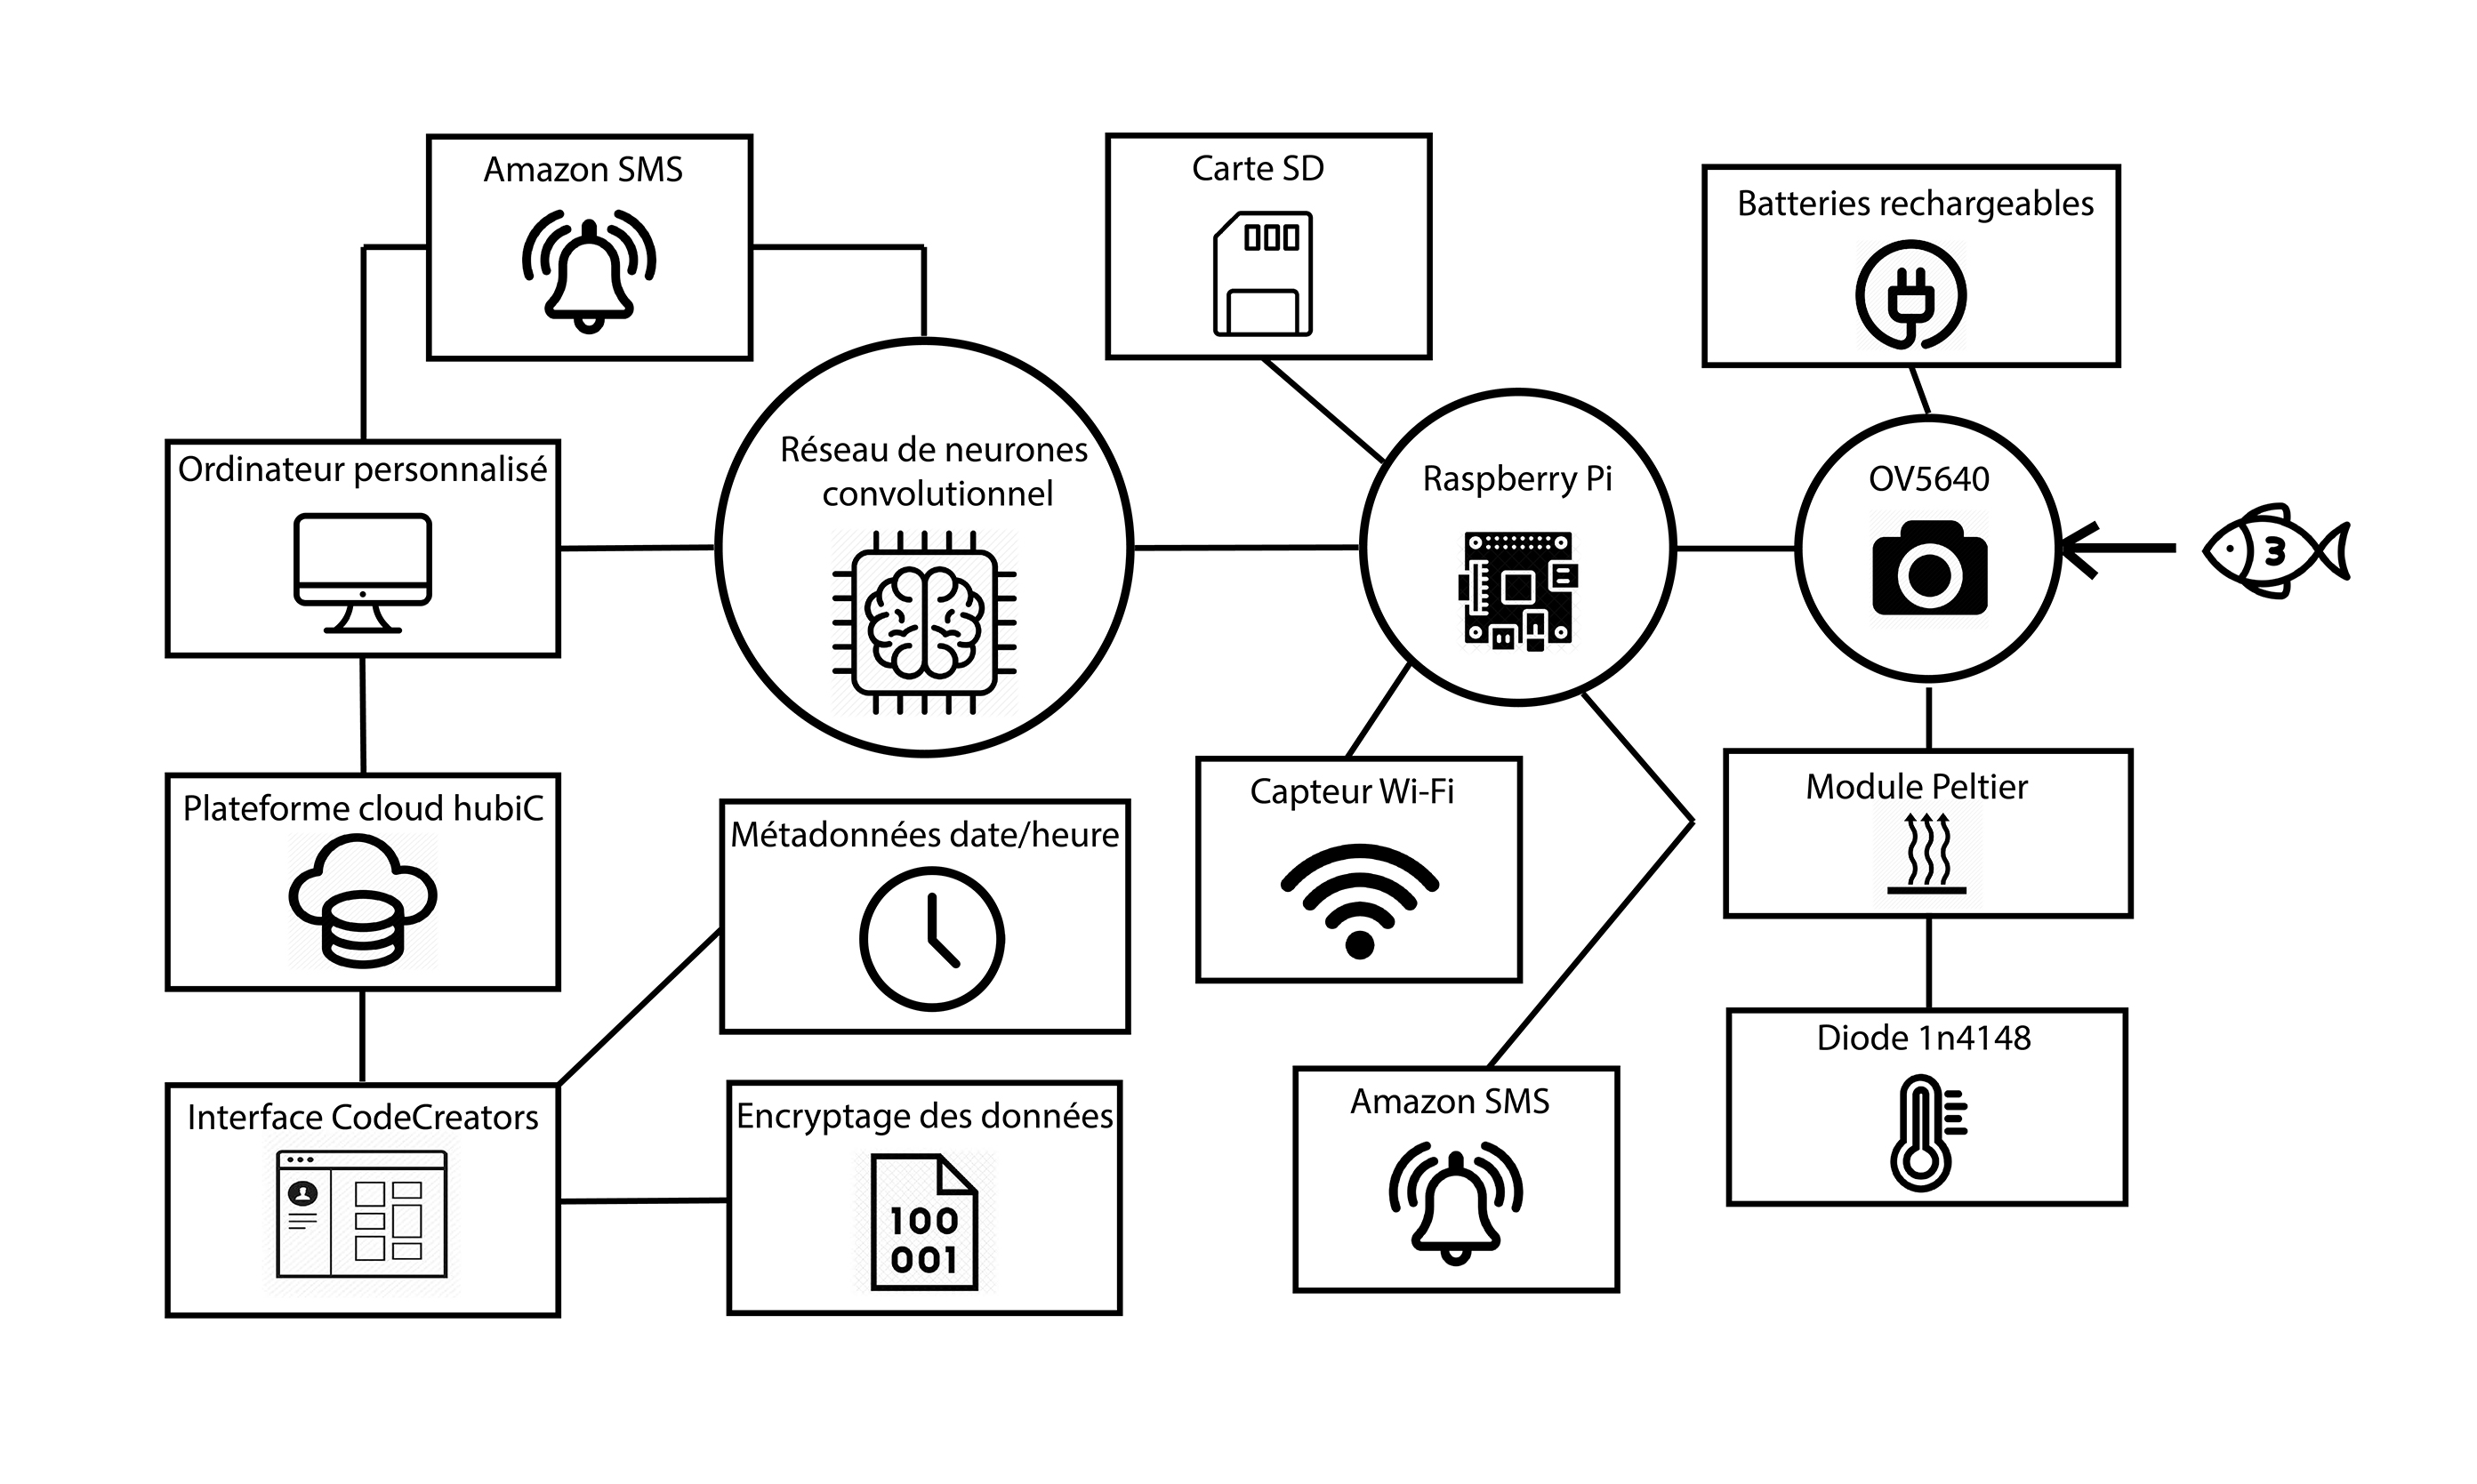
\includegraphics[width=\linewidth]{fig/schema_designnnnnn.jpg}
    \caption{Diagramme physique de la solution retenue pour le projet Fish \& Chips}
    \label{fig:concept_retenu}
\end{figure}


%!TEX encoding = IsoLatin

%
% Chapitre "Bibliographie"
%

\begin{thebibliographyUL}{9} % remplacer le "{9}" par "{99}" lorsque le nombre de references
                              % requiert 2 caracteres (>= 10 references)

\bibitem{Lac_walker} Ministère des Forêts, de la Faune et des Parcs du Québec, \emph{Projet de parc national du Lac Walker}, 2018. Référence accessible sur le site du MFFP: \url{https://mffp.gouv.qc.ca/les-parcs/reseau-parcs-nationaux/projet-de-parc-national-du-lac-walker/}.

\bibitem{Esturgeon} Pêches et Océans Canada, \emph{Esturgeon jaune (populations des Grands Lacs et du haut Saint-Laurent)}, 2018-09-06. Référence accessible sur le site du MPO: \url{https://mffp.gouv.qc.ca/les-parcs/reseau-parcs-nationaux/projet-de-parc-national-du-lac-walker/}.

\bibitem{GoPro_Specs} GoPro, \emph{GoPro Hero7 Black Edition Tech Specs}, 2019. Référence accessible sur le site de GoPro: \url{https://shop.gopro.com/International/hero7-black/tech-specs?pid=CHDHX-701-master}

\bibitem{GoPro_Waterproof} GoPro, \emph{Are GoPro Cameras Waterproof Without a Housing?}, 2019. Référence accessible sur le site de GoPro: \url{https://gopro.com/help/articles/question_answer/are-gopro-cameras-waterproof-without-a-housing}

\bibitem{HP2W} Reconyx, \emph{HP2W HYPERFIRE 2 PROFESSIONAL WHITE FLASH CAMERA}, 2015. Référence accessible sur le site de Reconyx: \url{http://www.reconyx.com/product/hyperfire-2-Professional-white-flash-camera}

\bibitem{GoFishCam} GoFishCam, \emph{The Camera}, 2018. Référence accessible sur le site de GoFishCam: \url{https://gofishcam.com/}

\bibitem{OV5640} ELP, \emph{FULL HD 5MP AUTOFOCUS USB CAMERA MODULE USB2.0 OV5640 COLOR CMOS SENSOR 60DEGREE LENS}, 2019. Référence accessible sur le site de ELP: \url{http://www.elpcctv.com/full-hd-5mp-autofocus-usb-camera-module-usb20-ov5640-color-cmos-sensor-60degree-lens-p-217.html}

\bibitem{OV5640_coûts} Alibaba, \emph{ELP Cmos ov5640 Mjpeg 5megapixel YUYuvc android linux windows free driver micro mini usb camera cmos chip ELP-USB500W02M-L36}, 2019. Référence accessible sur le site d'alibaba: \url{https://www.alibaba.com/product-detail/ELP-Cmos-ov5640-Mjpeg-5megapixel-YUYuvc_60119420904.html?spm=a2700.7724857.normalList.12.67586accCecTZ0}

\bibitem{ASM} ASM Aerospace Specification Data, \emph{Aluminium}. Référence accessible sur le site ASM: \url{http://asm.matweb.com/search/SpecificMaterial.asp?bassnum=MA2014T6&fbclid=IwAR3Zc5Insdhjf5uAf3x42XuvAWj6jC0X41uX9PkSsgZ-E6stMBCea0scOXs}

\bibitem{Glass} Information sheet "Glass and Acrylic glass", 2017. Référence accessible à l'adresse suivante: \url{https://www.chillventa.de/cmsfile/111/41/dd0f9e4d-4248-4ca4-80ac-875e5e195c6f--data/i4.8_2017_GB.pdf}

\bibitem{Ajax_wiki} Wikipédia, \emph{Ajax (programming)}, 2019. Référence accessible sur le site de Wikipédia: \url{https://en.wikipedia.org/wiki/Ajax_(programming)}

\bibitem{Ajax} Keycdn, \emph{What is Ajax Programming - Explained}, 2018. Référence accessible sur le site de Keycdn: \url{https://www.keycdn.com/support/ajax-programming}

\bibitem{Csoft} Csoft Technology, \emph{Ajax Development}, 2019. Référence accessible sur le site de Csoft Technology: \url{http://www.csofttech.com/ajax-development.html}

\bibitem{PF_exemple} Oracle, \emph{PrimeFaces in the Enterprise}, 2014. Référence accessible sur le site de Oracle: \url{https://www.oracle.com/technetwork/articles/java/java-primefaces-2191907.html}

\bibitem{PF_Roma} PrimeFaces, \emph{Roma}, 2019. Référence accessible sur le site de PrimeFaces: \url{https://www.primefaces.org/layouts/roma}

\bibitem{PF} PrimeFaces, 2019. Référence accessible sur le site de PrimeFaces: \url{https://www.primefaces.org/}

\bibitem{Comentum} Comentum, \emph{Web Application Devolopment Services}, 2019. Référence accessible sur le site de Comentum: \url{https://www.comentum.com/web-application-development-services.html}

\bibitem{Dev_salary} Neuvoo, \emph{Salaire Développeur web, Canada}, 2019. Référence accessible sur le site de Neuvoo: \url{http://neuvoo.ca/salaire/?job=developpeur+web}

\bibitem{CodeCreators} CodeCreators, \emph{Mobile App Development}, 2019. Référence accessible sur le site de CodeCreators: \url{https://www.codecreators.ca/mobile-application-development/}

\bibitem{CodeCreators2} CodeCreators, \emph{IOT Development}, 2019. Référence accessible sur le site de CodeCreators: \url{https://www.codecreators.ca/iot-development/}

\bibitem{Photographic_optics} A.R. Greenleaf, \emph{Photographic optics}, 1950. Référence accessible sur le site Google books: \url{https://books.google.ca/books?id=M5ghAAAAMAAJ}

\bibitem{Ares} Fiche descriptive du thermomètre Accu-Temp sur le site Arescuisine, Référence accessible sur le site: \url{https://www.arescuisine.com/us/thermometre-numerique-bluetooth-android-apple-accu.html}

\bibitem{AmAc} Fiche descriptive du thermomètre Accu-Temp sur le site d'Amazon : \url{https://www.amazon.ca/Accu-Temp-Smart-Cooking-Thermometer/dp/B01N0GWF1R}
\bibitem{CaAc}Fiche descriptive du thermomètre Accu-Temp sur le site du magasin Canadian Tire:
\url{https://www.canadiantire.ca/fr/pdp/accu-temp-smart-cooking-thermometer-1424307p.html}

\bibitem{TuAr} Tutoriel sur l’utilisation de la thermistance avec Arduino : 
\url{http://www.circuitbasics.com/arduino-thermistor-temperature-sensor-tutorial/}

\bibitem{DaTh} Fiche de la thermistance NTCLE100E3103JT2 sur digikey :
\url{https://www.digikey.ca/product-detail/en/vishay-bc-components/NTCLE100E3103JT2/BC2396TR-ND/2230724}

\bibitem{AmAr}Fiche de l’Arduino Uno sur le site d’amazon :
\url{https://www.amazon.com/Arduino-A000066-ARDUINO-UNO-R3/dp/B008GRTSV6}

\bibitem{Thermo}Fiche de présentation du thermomètre intelligent Thermo de Withings :
\url{https://www.withings.com/ca/fr/thermo?gclid=Cj0KCQjwg73kBRDVARIsAF-kEH8n85xIN_s-bC4XwdGrTSWUHH0uYsVg_0Vvm2RqW8_NIj5mhevLMp4aAivFEALw_wcB&gclsrc=aw.ds}

\bibitem{Allie} Fiche de vente de la diode 1n4148 sur alliedelec.com :
\url{https://ca-en.alliedelec.com/product/vishay-small-signal-opto-products-ssp-/1n4148-tr/70061726/?&gclid=Cj0KCQjwg73kBRDVARIsAF-kEH-W0AxulJrrerGKhb8asdrQz38ZbRS-QWP_tOYEOEv7whkFbtyOT4AaAujYEALw_wcB&gclsrc=aw.ds}

\bibitem{Tu1n} Tutoriel de l’utilisation d’un Arduino et d’une diode 1n4148 comme thermomètre :
\url{https://www.hackster.io/microst/thermometer-diode-based-524613}
\bibitem{Da1n} Fiche technique de la diode 1n4148 :
\url{https://www.vishay.com/docs/81857/1n4148.pdf}

\bibitem{amsd} Fiche de la carte SD SanDisk 32 Go classe 10 sur le site de vente en ligne Amazon :
\url{https://www.amazon.ca/Sandisk-Ultra-Class-Memory-SDSDUNC-032G-GN6IN/dp/B0143RT8OY/ref=sr_1_1?adgrpid=64072851822&hvadid=338546225427&hvdev=c&hvlocphy=9000264&hvnetw=g&hvpos=1t1&hvqmt=b&hvrand=1385930668605963580&hvtargid=kwd-311568263496&keywords=sd+card+32gb&qid=1553004425&s=gateway&sr=8-1&tag=googlefrenchd-20}

\bibitem{casd} Fiche de la carte SD SanDisk 32 Go classe 10 sur le site de Canadian Tire :
\url{https://www.canadiantire.ca/fr/pdp/carte-memoire-sd-sandisk-32-go-classe-10-0694082p.html?gclid=Cj0KCQjwpsLkBRDpARIsAKoYI8y8O4isWSxEqKLtHY_QyjSDdHdr_cnhVIpC60UhN_DvTz08a23cfiEaAnVeEALw_wcB&gclsrc=aw.ds}

\bibitem{hubic} Site internet de hubic :
\url{https://hubic.com/fr/}

\bibitem{clgo} Site internet de la plateforme nuage de Google :
\url{https://cloud.google.com/gcp/?hl=fr&utm_source=google&utm_medium=cpc&utm_campaign=na-CA-all-fr-dr-bkws-all-all-trial-e-dr-1006141&utm_content=text-ad-none-any-DEV_c-CRE_246981386096-ADGP_Hybrid\%20\%7C\%20AW\%20SEM\%20\%7C\%20BKWS\%20\%7C\%20CA\%20\%7C\%20fr\%20\%7C\%20Multi\%20~\%20Google\%20Cloud-KWID_43700029712638740-kwd-6458750523&utm_term=KW_google\%20cloud-ST_google\%20cloud&gclid=Cj0KCQjwpsLkBRDpARIsAKoYI8y55-FY-u-tbcMjyD27TnRNwxsovqkawa7ihIos6lvoeZUJhV6wZkIaAlmxEALw_wcB}

\bibitem{incl} Description des systèmes informatique en nuage :
\url{https://www.pmtic.net/sites/default/files/filemanager/memos/pmtic_rech_stock_orga_stocker_cloud.pdf}

\bibitem{AMSSD}Fiche du disque dur SSD Kingstone Digital SSD A400 SATA 3 sur le site de vente en ligne Amazon :
\url{https://www.amazon.ca/Kingston-Digital-240GB-SA400S37-240G/dp/B01N0TQPQB/ref=sr_1_1?adgrpid=70588794910&hvadid=338566747399&hvdev=c&hvlocphy=9000264&hvnetw=g&hvpos=1t1&hvqmt=e&hvrand=7332898350628790834&hvtargid=kwd-6250669858&keywords=ssd\%2Bhard\%2Bdrive&qid=1553010981&s=gateway&sr=8-1&tag=googlefrenchd-20&th=1}

\bibitem{DESSD} Description des disques durs sur SSD :
\url{https://www.culture-informatique.net/cest-quoi-disque-dur-ssd/}

\bibitem{HDD1} Fiche du disque dur Western Digital SATA III sur Amazon :
\url{https://www.amazon.ca/Western-Digital-Cache-Desktop-Drive/dp/B0088PUEPK/ref=sr_1_2?adgrpid=66673166829&hvadid=338547656331&hvdev=c&hvlocphy=9000264&hvnetw=g&hvpos=1t1&hvqmt=e&hvrand=10837815785367396351&hvtargid=kwd-15026630&keywords=hdd&qid=1553028630&s=gateway&sr=8-2&tag=googlefrenchd-20}

\bibitem{HDD2} Article traitant de la différence entre disque dur HDD et SDD :
\url{https://blog.touchedeclavier.com/differences-entre-disque-dur-hdd-ssd/}

\bibitem{mercure} Fiche de vente du thermommètre H-B Instrument 2/1110 Durac sur Amazon :
\url{https://www.amazon.ca/Instrument-General-Immersion-Thermometer-Accuracy/dp/B00551N8Q2/ref=sr_1_2?__mk_fr_CA=\%C3\%85M\%C3\%85\%C5\%BD\%C3\%95\%C3\%91&keywords=mercury+thermometer&qid=1553089659&s=gateway&sr=8-2}

\bibitem{PMMA_cout} \emph{ACRYLIC SHEET PRICES} San Diego Plastics Inc. Fiche de vente du PMMA: \url{http://www.sdplastics.com/sdplas2.html}


\bibitem{Aluminium_cout} \emph{Aluminium 2014 T6 Plate Suppliers} Sanghvi Overseas Inc. Fiche de vente des plaques d'aluminium: \url{https://www.sanghvioverseasinc.com/aluminium-aluminum/aluminium-plate-aluminum-plate/aluminium-2014-t6-plate-manufacturer-supplier/}

\bibitem{RF_eau} Qureshi, Umair Mujtaba et al. “RF Path and Absorption Loss Estimation for Underwater Wireless Sensor Networks in Different Water Environments” Sensors (Basel, Switzerland) vol. 16,6 890. 16 Jun. 2016, doi:10.3390/s16060890.  \url{https://www.ncbi.nlm.nih.gov/pmc/articles/PMC4934316/}

\bibitem{eau1} Article traintant du refroidissement à eau :
\url{http://hmf.enseeiht.fr/travaux/CD0102/travaux/optemf/bei_mot/0102/pages/piston/partieb/refroid/intro.htm}

\bibitem{eau2} Fiche de la vente du EK-KIT-S120 sur le site EKWB :
\url{https://www.ekwb.com/shop/ek-kit-s120}

\bibitem{iPhone7} Fiche de vente du iPhone 7: \url{https://www.apple.com/xf/shop/buy-iphone/iphone-7}

\bibitem{rad1} Article traitant des radiateurs de moteurs d'automobiles :
\url{https://westislandgarage.com/reparation-automobile/circuit-de-refroidissement-du-moteur/}

\bibitem{rad2} Fiche de vente du radiateur ABAKUS :
\url{https://www.piecesauto24.com/abakus/8528530}

\bibitem{pate1} Article traitant des pâtes thermiques
\url{https://www.config-gamer.fr/guide-achat/quelle-pate-thermique-choisir-pour-refroidir-votre-processeur-7222.html}

\bibitem{pate2} Fiche de vente de la pâte NT-H1 sur le site de vente en ligne cdisount.com :
\url{https://www.cdiscount.com/informatique/ventilation-refroidissement/noctua-pate-thermique-nt-h1/f-10789-nth1.html?awc=6948_1553134427_6df016c478eb94c9b40e818aa23e8c09&refer=zanoxpb&cid=affil&cm_mmc=zanoxpb-_-297939}

\bibitem{pel1} Article traitant des modules Peltier :
\url{https://www.digikey.fr/fr/articles/techzone/2018/feb/choosing-using-advanced-peltier-modules-thermoelectric-cooling}

\bibitem{pel2} Fiche de vente du module Peltier Tec1-12706 :
\url{https://www.banggood.com/fr/TEC1-12706-40x40mm-Thermoelectric-Cooler-Peltier-Plate-Module-12V-60W-p-74295.html?rmmds=detail-top-buytogether-auto&cur_warehouse=USA}

\bibitem{usb_50m} Lindy International \url{https://www.lindy-international.com/USB-3-0-AOC-Cable-50m.htm?websale8=ld0101.ld020102&pi=42684}

\bibitem{usb_standard_50m} KVM Switches Online \url{https://www.kvm-switches-online.com/usb2-aa-50m.html}

\bibitem{Techflex} Techflex \url{https://www.wirecare.com/category/braided-sleeving/heavy-duty/flexo-heavy-wall?utf8=\%E2\%9C\%93&id=19&order=Price} \url{https://www.techflex.com/heavy-duty/flexo-heavy-wall?part=HWN0.13BK}

\bibitem{Raspberry_Pi} Raspberry Pi \url{https://www.raspberrypi.org/}

\bibitem{Routeur} LDLC \url{https://www.ldlc.com/fiche/PB00222375.html}

\bibitem{eau_EM} \emph{RF Path and Absorption Loss Estimation for Underwater Wireless Sensor Networks in Different Water Environments} \url{https://www.ncbi.nlm.nih.gov/pmc/articles/PMC4934316/}

\bibitem{Datetime} Librairie standard Python \url{https://docs.python.org/2/library/datetime.html}

\bibitem{Timer} Mini RTC \url{https://thepihut.com/products/mini-rtc-module-for-raspberry-pi}


\end{thebibliographyUL}

%   Annexes
\appendix
%!TEX encoding = IsoLatin

%
% Annexe "Liste des sigles et des acronymes"
%

\chapter{Liste des sigles et des acronymes}

% Ne pas y inclure les unités SI

\begin{flushleft}
   \begin{tabular}{@{}ll}
      API & Application Programming Interface \\
      BIPM & Bureau international des poids et mesures\\
      CGPM & Conférence générale des poids et mesures\\
      CODATA & Committee on Data for Science and Technology\\
      EM & Électromagnétique\\
      ISBN & International Standard Book Number\\
      JPEG & Joint Photographic Experts Group\\
      Mbps & Mégabits par seconde \\
      Mpx & Megapixel \\
      MFA & Ministère de la Faune Aquatique \\
      NIST & National Institute of Standards and Technology \\
      PDF & Portable Document Format \\
      PET & Polytéréphtalate d'éthylène \\
      PMMA & Polyméthacrylate de méthyle \\
      RADARSAT & RADAR SATellite\\
      RF & Fréquences radios\\
      SI & Système international d'unités \\
      URL & Uniform Resource Locator \\
   \end{tabular}
\end{flushleft}







%!TEX encoding = IsoLatin

%
% Annexe "Équations de la caméra custom"
%

\chapter{Équations pour le capteur d'image OV5640}
\label{annexe:equation_camera_custom}

Dans cette annexe, toutes les équations nécessaires à la compréhension des données de la section \ref{subsubsection:camera_custom} seront fournies.

Les spécifications du fabriquants nécessaires aux calculs sont indiqués au tableau \ref{t:specs_camera_custom}.

\begin{table}[!htb]
\footnotesize
\centering
    \begin{tabular}{|c|c|}
    \hline
    Specs & Valeur\\
    \hline\hline
    Taille du pixel & 1.4$\mu$m\\
    Hauteur du senseur ($H$) & 2738.4 $\mu$m\\
    Largeur du senseur ($W$) & 3673.6 $\mu$m\\
    Focale & 3.2mm\\
    F-number & 2.8\\
    \hline
    \end{tabular}
\caption{Spécification du fabriquant pour le capteur OV5640 \cite{OV5640}}
\label{t:specs_camera_custom}
\end{table}

Pour l'exemple de calcul, les données suivantes du tableau \ref{t:ex_calcul_camera_custom} seront considérées. Celles-ci sont possible selon les données fournies par le fabriquant. Le diamètre de la lentille est déterminé à partir du F-number $N=f/D$ et le cercle de confusion est calculé comme $c=1.5 t_\text{px}$
\begin{table}[!htb]
\footnotesize
\centering
    \begin{tabular}{|c|c|}
    \hline
    Specs & Valeur\\
    \hline\hline
    Focale ($f$) & 3.2mm\\
    F-number ($N$) & f/2.8\\
    Diamètre de la lentille ($D$) & 1.143mm\\
    Distance du focus ($s$) & 1.0m\\
    Distance lentille-capteur ($d$) & 3.2mm\\
    Cercle de confusion ($c$) &  2.1 $\mu$m\\
    \hline
    \end{tabular}
\caption{Valeurs pour un exemple de calcul}
\label{t:ex_calcul_camera_custom}
\end{table}

Les équations \ref{eq:distance_hyperfocale} à \ref{eq:champ_lointain} sont les équations d'imagerie \cite{Photographic_optics}. La distance hyperfocale $H$ est une nécessaire pour calculer la profondeur de champ:
\begin{equation}
    H = \frac{f^2}{Nc} - f
    \label{eq:distance_hyperfocale}
\end{equation}

Le champ proche $D_n$ est la limite inférieure à laquelle le système peut imager:
\begin{equation}
    D_n = \frac{s(H-s)}{H+s-2f}
    \label{eq:champ_proche}
\end{equation}

Le champ lointain $D_f$ est la limite supérieure à laquelle le système peut imager:
\begin{equation}
    D_n = \frac{s(H-s)}{H-s}
    \label{eq:champ_lointain}
\end{equation}

\begin{figure}[!htb]
    \centering
    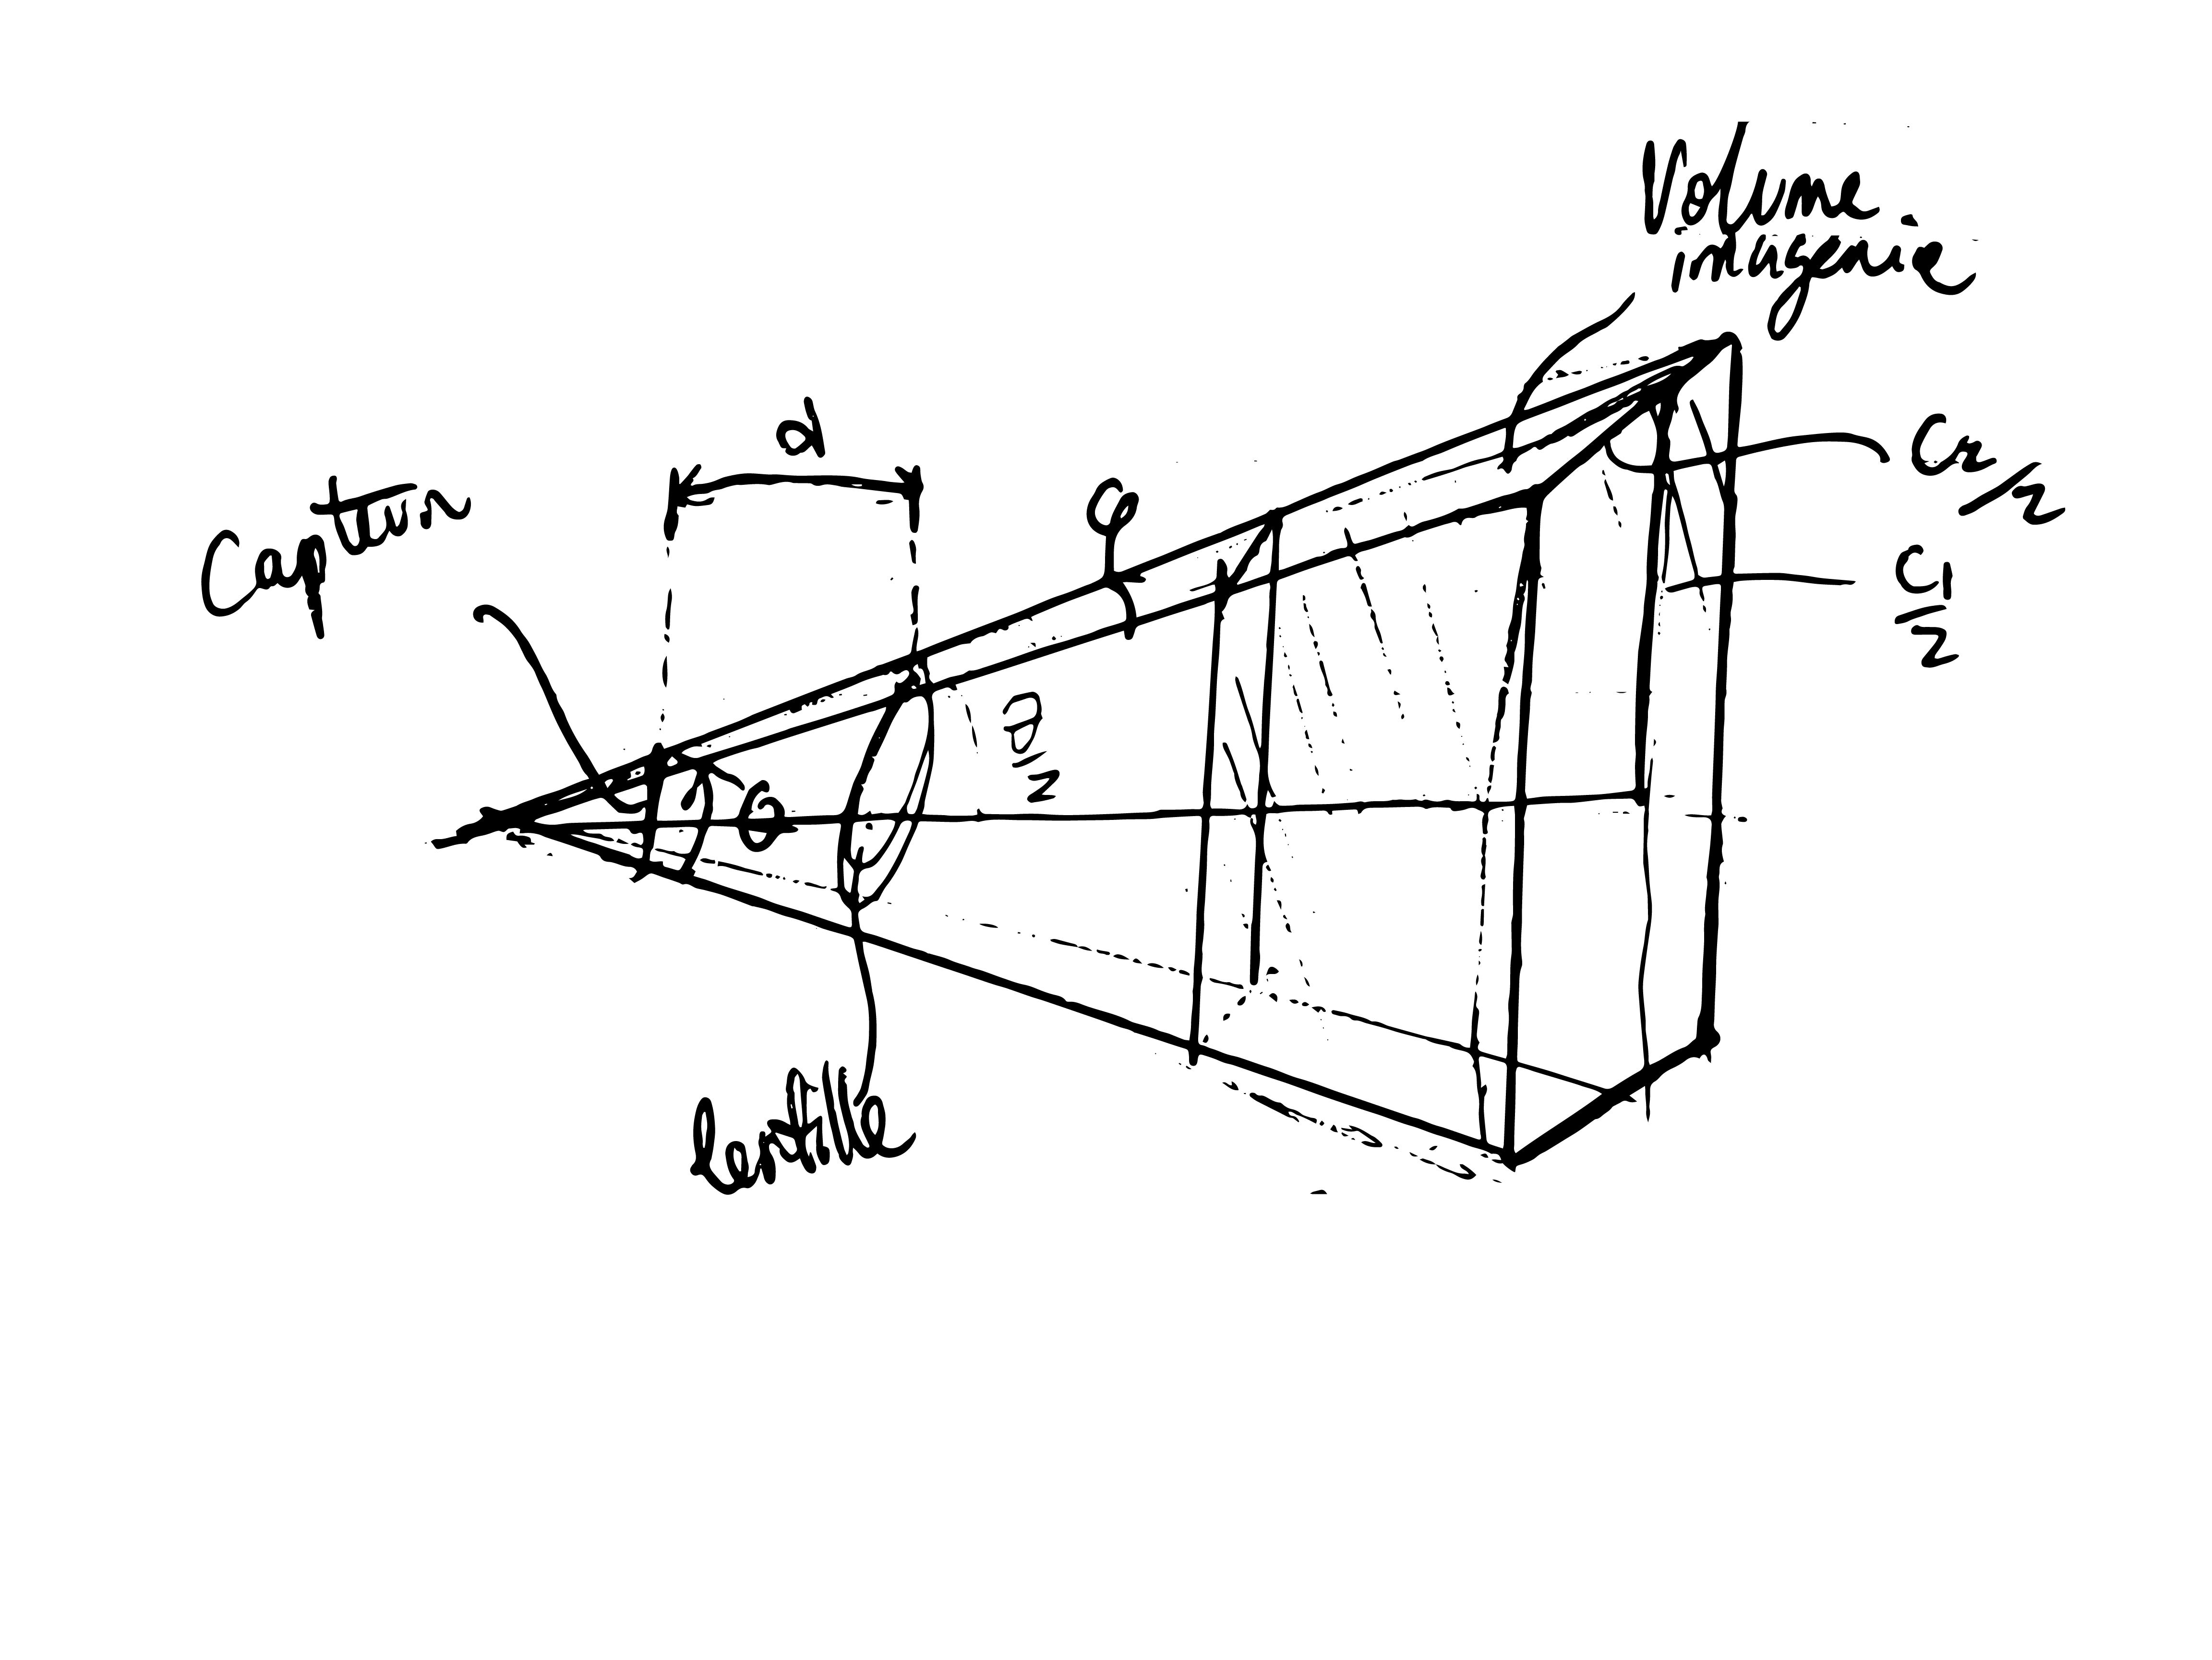
\includegraphics[width=0.5\linewidth]{fig/camera_custom_geometrie_vect.png}    \caption{Géométrie du volume d'imagerie}
    \label{fig:volume_imagerie}
\end{figure}


Le volume d'imagerie est une pyramide tronquée. Le développement de son équation nécessite donc les équations d'imagerie et les équations de la géométrie du système. Les équations \ref{eq:base_lointaine} à \ref{eq:angles} définissent la géométrie du système à la figure \ref{fig:volume_imagerie}. L'aire de la base la plus lointaine $Ab_f$ est définie un rectangle tel que
\begin{align}
    Ab_f &= c_{1f} \cdot c_{2f}\\
    c_{1f} &\equiv 2D_f \tan{\frac{\theta}{2}}\\
    c_{2f} &\equiv 2D_f \tan{\frac{\phi}{2}}\\
    Ab_f &= (2 D_f)^2 \tan{\frac{\theta}{2}} \tan{\frac{\phi}{2}}
    \label{eq:base_lointaine}
\end{align}

L'aire de la base la plus proche $Ab_n$ est définie un rectangle tel que
\begin{align}
    Ab_n &= c_{1n} \cdot c_{2n}\\
    c_{1n} &\equiv 2D_n \tan{\frac{\theta}{2}}\\
    c_{2n} &\equiv 2D_n \tan{\frac{\phi}{2}}\\
    Ab_n &= (2 D_n)^2 \tan{\frac{\theta}{2}} \tan{\frac{\phi}{2}}
    \label{eq:base_proche}
\end{align}


\begin{figure}[!htb]
    \centering
    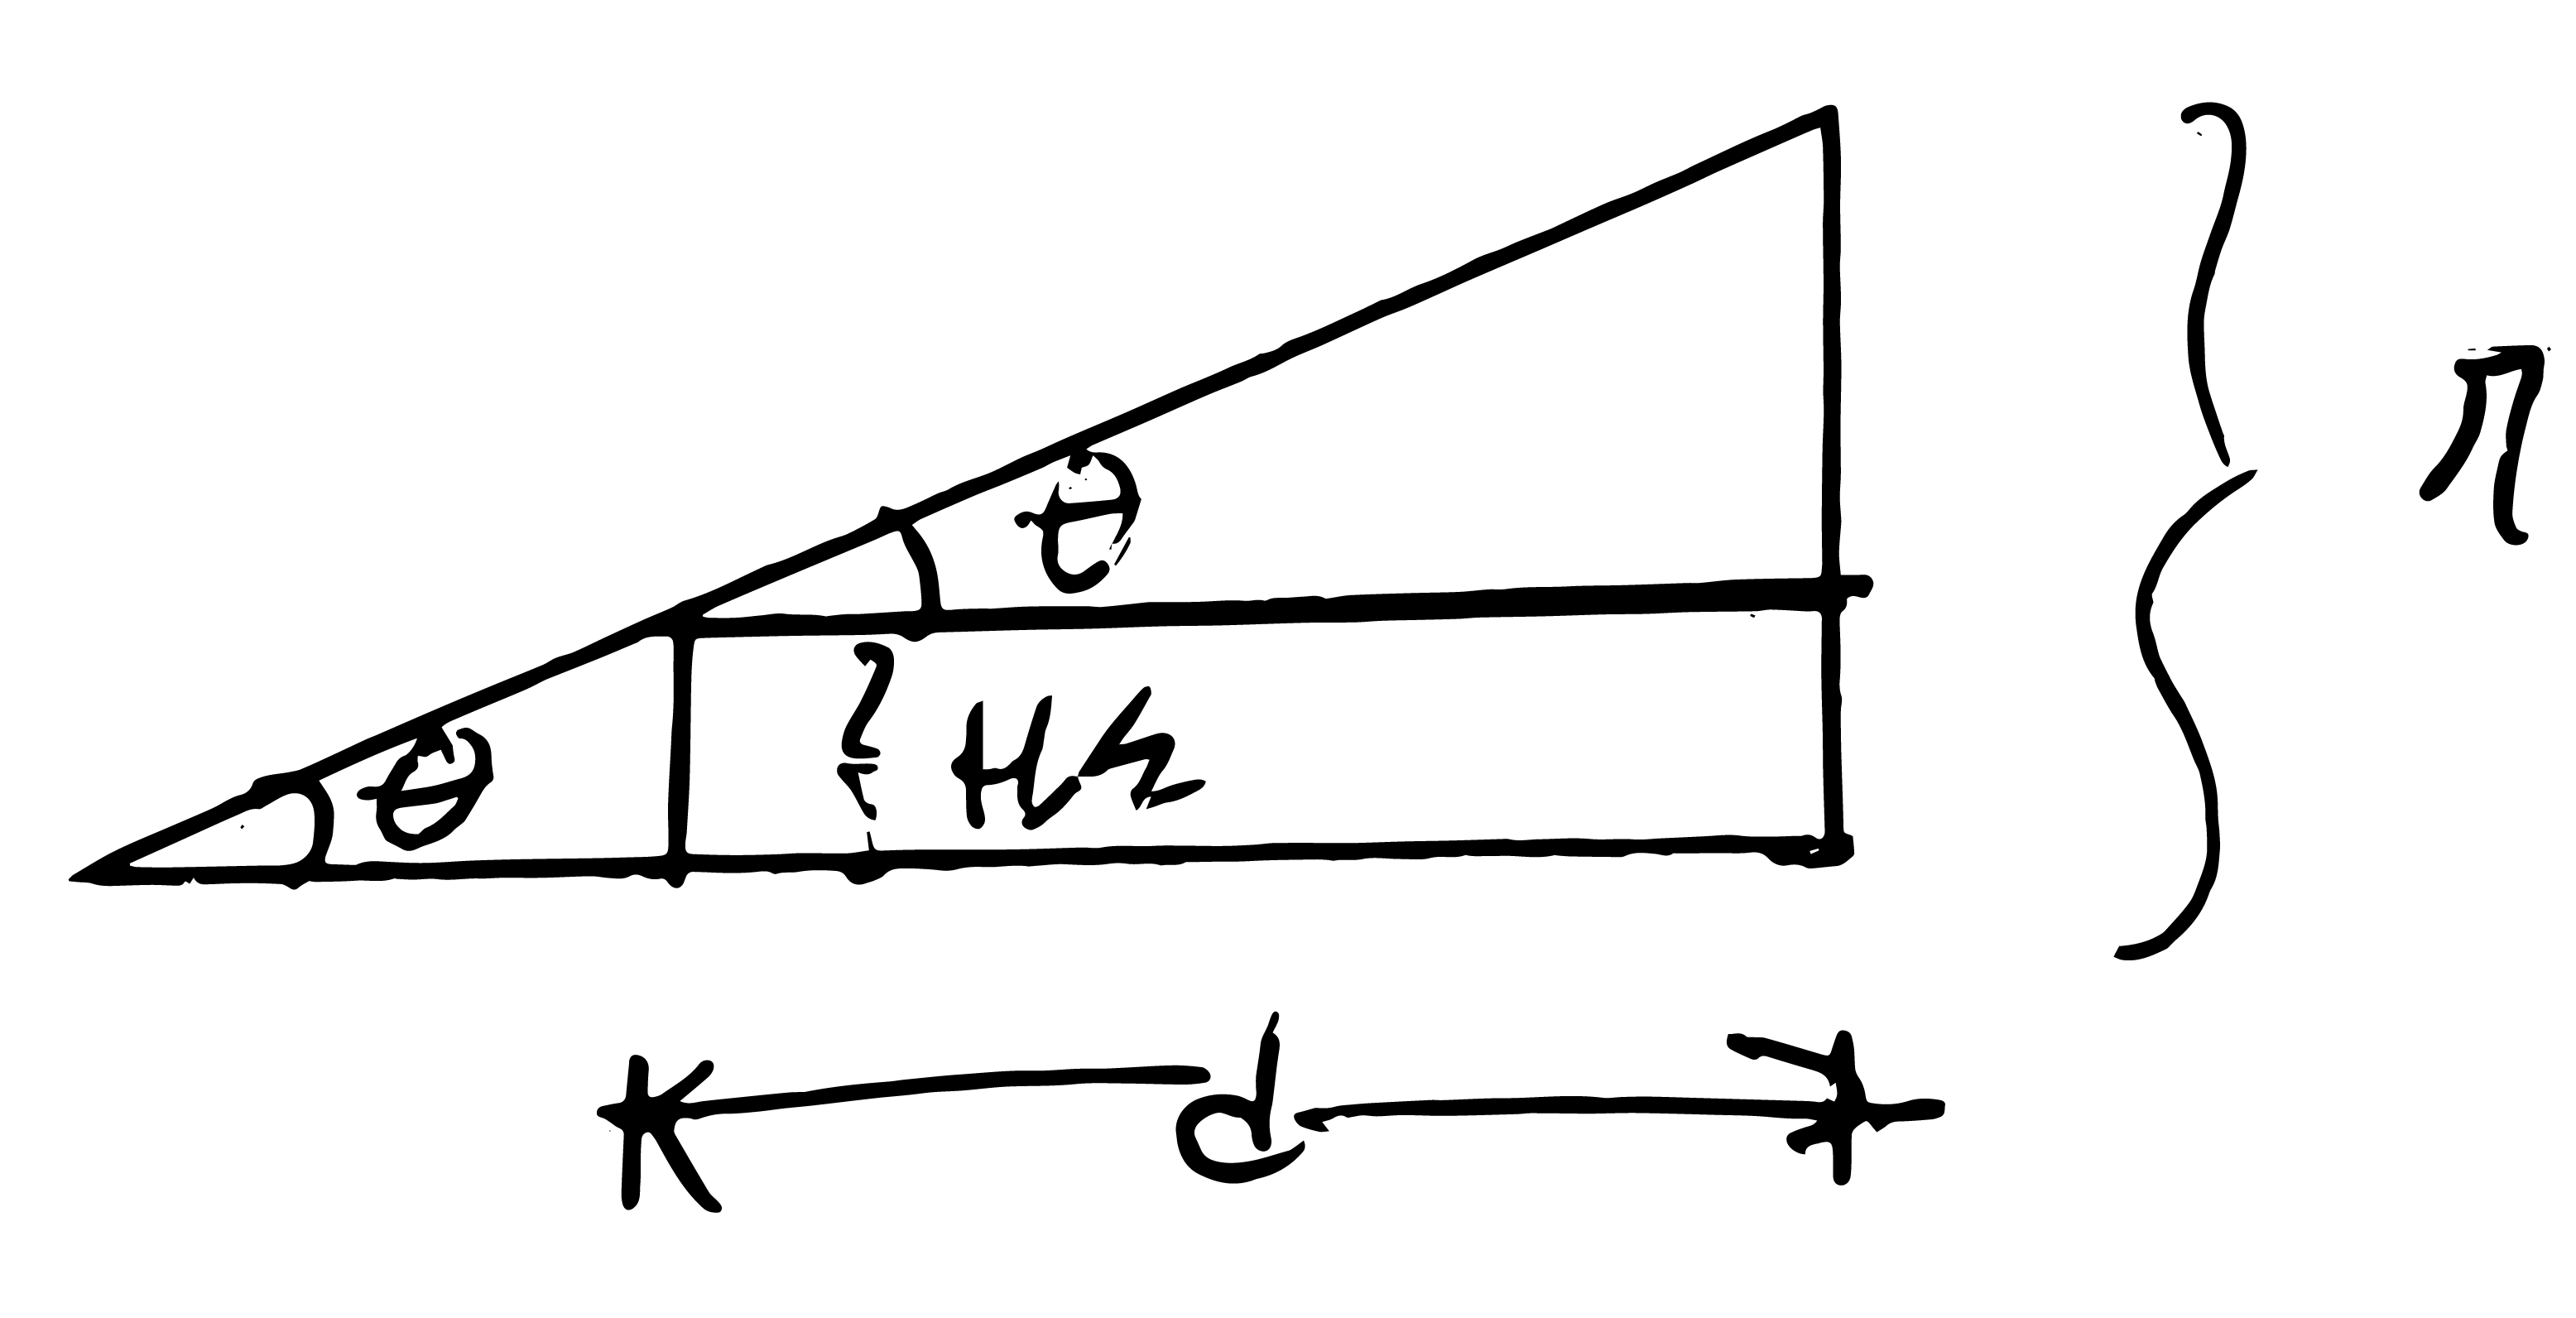
\includegraphics[width=0.5\linewidth]{fig/camera_custom_angle_vect.png}
    \caption{Géométrie du système lentille-capteur}
    \label{fig:lentille_capteur}
\end{figure}

À l'aide du système lentille-capteur, il est possible de déterminer une relation pour les angles $\phi$ et $\theta$ en supposant que l'ouverture du champ est limitée par le diamètre de la lentille.
\begin{align}
    \tan{\frac{\theta}{2}} &= \frac{r-H/2}{d}\\
    \tan{\frac{\theta}{2}} &= \frac{D-H}{2d}\\
    \tan{\frac{\phi}{2}} &= \frac{r-W/2}{d}\\
    \tan{\frac{\theta}{2}} &= \frac{D-W}{2d}
    \label{eq:angles}
\end{align}

En combinant toutes ces équations, il est possible d'arriver à la relation suivante:
\begin{align}
    V &= \frac{Ab_f D_f}{3} - \frac{Ab_n D_n}{3}\\ 
    V &= \frac{4 \tan{\frac{\theta}{2}}  \tan{\frac{\phi}{2}}}{3} \left( D_f^3 - D_n^3\right)\\
    V &= \frac{4}{3} \left(\frac{D-H}{2d} \right) \left(\frac{D-W}{2d} \right) \left( D_f^3 - D_n^3\right)
    \label{eq:volume_imagerie}
\end{align}

On obtient alors les résultats montrés au tableau \ref{t:resultat_calcul_camera_custom}.
\begin{table}[!htb]
\footnotesize
\centering
    \begin{tabular}{|c|c|}
    \hline
    Specs & Valeur\\
    \hline\hline
    Hyperfocale & 1.738m\\
    Limite de champ proche $D_n$ & 0.635m\\
    Limite de champ lointain $D_f$ & 2.350m\\
    Angle d'ouverture $\theta$ & -27.997°\\
    Angle d'élévation $\phi$ & -43.151°\\
    Volume d'imagerie & 1.672m$^3$\\
    \hline
    \end{tabular}
\caption{Résultat de l'exemple de calcul}
\label{t:resultat_calcul_camera_custom}
\end{table}


\chapter{Équations pour le boitier}
\label{annexe:equation_boitier}

La pression hydrostatique est définie à l'équation \ref{eq:profondeur}. La profondeur est $h$ et $p_0$ est la pression atmosphérique.

\begin{equation}
    p = p_0 +\gamma_\text{eau} h
    \label{eq:profondeur}
\end{equation}

Ainsi, la pression à une profondeur de 15.25m est de 250.9kPa.

\begin{align}
    p &= p_0 +\gamma_\text{eau} h\\
    &= 101.3\text{kPa} + 9.807\text{kN/m}^3 \cdot 15.25m\\
    &= 101.3\text{kPa} + 149.6\text{kPa}\\
    p &= 250.9\text{kPa}
\end{align}

Selon le design du boitier à la figure \ref{fig:boitier_camera_custom}, les caractéristiques seraient les suivantes 

\begin{table}[!htb]
\footnotesize
\centering
    \begin{tabular}{|c|c|c|}
    \hline
    Caractéristique & Aluminium & PMMA\\
    \hline\hline
    Surface & 6$\cdot$ 0.04m$^2$ & 0.04m$^2$\\
    Épaisseur & 6mm & 2mm\\
    Masse pour la commande & 4.032kg & 0.095kg\\
    Coût & 2.6\$/kg & 3.70\$/ft$^2$ \\
    \hline
    Coût total & 10.50\$ & 1.59\$ \\
    \hline
    \end{tabular}
\caption{Caractéristiques pour la commande des matériaux du boitier \cite{PMMA_cout} \cite{Aluminium_cout}}
\label{t:commande_boitier}
\end{table}

La masse d'aluminium dans le dispositif est
\begin{align}
    m &= \rho_{Al} V\\
    V &= c^3 - (c-t)^3\\
    V &= (0.2m)^3 - (0.2m - 0.006m)^3\\
    V &= 6.99 \cdot 10^{-4} m^3\\
    m &= 2800 kg/m^3 \cdot 6.99 \cdot 10^{-4}m^3\\
    m &= 1.956 kg
\end{align}

La masse de PMMA dans le dispositif est
\begin{align}
    m &= \rho_{PMMA} V\\
    V &= \pi r^2 t\\
    V &= \pi (0.075m)^2 (0.002m)\\
    V &= 3.53 \cdot 10^{-5} m^3\\
    m &= 1190 kg/m^3 \cdot 3.53 \cdot 10^{-5} m^3\\
    m &= 0.042 kg
\end{align}

Le boitier aurait donc une masse de 2.00kg.

\chapter{}

\section{Équations pour la caméra Hyperfire HP2W}
\label{annexe:eq_hyperfire}

Selon les données du fabricant, le flash émis par la caméra peut se rendre jusqu'à 100 pieds \cite{HP2W}. Par contre, il faut imager des poissons de 6cm alors c'est plutôt son pouvoir de résolution qui détermineras la distance maximale du volume d'imagerie.

La caméra Hyperfire HP2W a un capteur CMOS de 3MP avec un rapport hauteur largeur standard. En se fiant à un capteur CMOS 3MP standard, il est possible de déduire que la taille des pixels de la Hyperfire est de 2.2 $\mu$m \cite{CMOS_standard}. Puisque la focale est ajustable, on assume une focale de 3 mm. En reprenant l'équation \ref{eq:johnson}, la distance maximale à laquelle on peut imager un poisson de 6 cm est de 5.11 m.
\begin{align*}
    h &= 16t_\text{px} \frac{d_o}{f}\\
    0.06 &= 16 \cdot (2.2\cdot10^{-6}) \frac{d_o}{0.003}\\
    d_o &= 5.11\text{ m}
\end{align*}
En assumant un angle d'ouverture de 45° et un angle d'élévation de 30°, il est possible de trouver le volume d'imagerie avec l'équation \ref{eq:volume_imagerie} sachant que $D_f=5.11$ m et $D_n=0$ m.
\begin{align}
    V &= \frac{4}{3} \tan{\theta/2}\tan{\phi/2} (D_f^3-D_n^3)\\
    V &= 18.5\text{ m}^3
\end{align}
Il s'agit toutefois d'une approximation étant donné que les spécifications sur le diamètre de la lentille n'étaient pas fournies. La taille de poisson minimale que l'on peut résoudre serait cependant de 6 cm.

\section{Volume d'imagerie de la caméra GoFishCam}
\label{annexe:eq_gofishcam}
On peut reprendre la même logique pour la caméra GoFishCam. Elle est équipée d'une DEL pour la vision nocturne. Si la distance maximale d'imagerie n'est pas trop élevée, la lumière devrait se rendre.

Elle a une résolution d'environ 2 MP. En se fiant sur un senseur standard de 2 MP, la taille d'un pixel serait de 1.4 $\mu$m \cite{CMOS_standard_2MP}. On assume encore une fois une focale de 3 mm.
\begin{align*}
    h &= 16t_\text{px} \frac{d_o}{f}\\
    0.06 &= 16 \cdot (1.4\cdot10^{-6}) \frac{d_o}{0.003}\\
    d_o &= 8.036\text{ m}
\end{align*}
Puisque cette distance est plus grande, on peut réduire le volume d'imagerie pour être capable de résoudre des poissons un peu plus petits. De plus, la lumière de la GoFishCam est vert pour ne pas perturber les poissons puisque son utilisation première est pour la pêche. La lumière ne se rend probablement pas jusqu'à 5.11 m. On pose donc la distance de champ lointain à 3.0 m. Par contre, avec une telle distance, il sera possible de résoudre des poissons plus petits. En reprenant la même équation, on trouve que le poisson le plus petit que l'on peut résoudre aurait une taille de 2.24 cm.
\begin{align*}
    h &= 16 t_\text{px} \frac{d_o}{f}\\
    h &= 16 \cdot (1.4\cdot10^{-6}) \frac{3.0}{0.003}\\
    h &= 0.038 \text{ m}
\end{align*}
Le volume d'imagerie serait alors de 4.00 m$^3$.
\begin{align}
    V &= \frac{4}{3} \tan{\theta/2}\tan{\phi/2} (D_f^3-D_n^3)\\
    V &= 4\text{ m}^3
\end{align}
Il s'agit toutefois d'une approximation étant donné que les spécifications sur le diamètre de la lentille n'étaient pas fournies.
\chapter{Barèmes}
\label{annexe:baremes}

\section{Barème pour la sécurité}
\label{annexe:baremes_securite}

L'équation suivante donne une équation exponentielle où la droite passe nécessairement par ($a$,0) et ($c$,1). Le ratio $a/b$ peut être ajusté pour donner la forme voulue à la courbe.
\begin{equation}
    y(x) = \frac{e^{\frac{x-a}{b}-1}}{e^{\frac{c-a}{b}-1}}
    \label{annexe:bareme_sécurité}
\end{equation}

Dans le cas où $c=5$,

\begin{figure}[h]
    \centering
    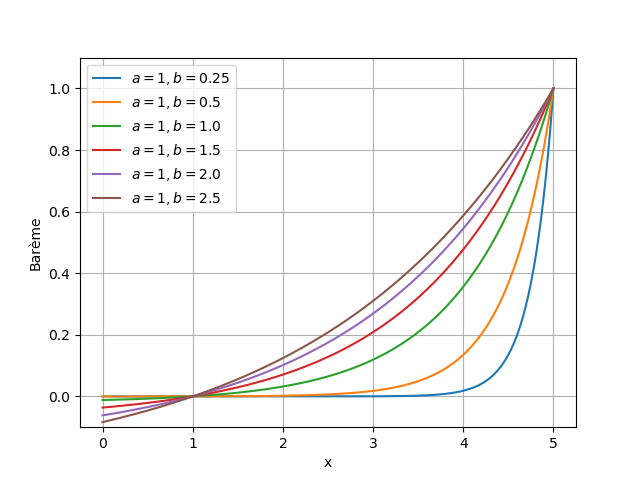
\includegraphics[width=0.75\linewidth]{fig/exp_securite.png}
    \caption{Barème exponentielle pour la sécurité}
    \label{fig:exp_securite}
\end{figure}

\section{Barème pour la taille des poissons}
\label{annexe:baremes_poisson}


L'équation suivante donne une équation exponentielle où la droite passe nécessairement par (0,1) et ($a$,0). Le ratio $a/b$ peut être ajusté pour donner la forme voulue à la courbe.
\begin{equation}
    y(x) = \frac{1-10^{\frac{x-a}{b}}}{1-10^{a/b}}
    \label{annexe:bareme_exp_poisson}
\end{equation}

\begin{figure}[h]
    \centering
    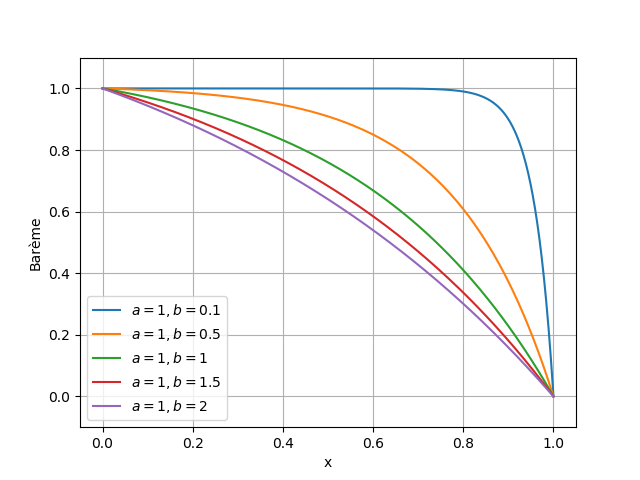
\includegraphics[width=0.75\linewidth]{fig/exp_poisson.png}
    \caption{Barème exponentielle pour la taille des poissons}
    \label{fig:exp_poisson}
\end{figure}




\end{document}
% Fin du document

